%\documentclass[smallabstract,smallcaptions]{dccpaper}
\documentclass[12pt,onecolumn,final,letterpaper]{IEEEtran}
%
\usepackage{amssymb,amsthm}
\usepackage{thmtools}
\usepackage{amsxtra,amsfonts}
\usepackage[dvipsnames]{xcolor}
\usepackage{enumitem}
\usepackage{mathtools}
\usepackage{enumitem}
\usepackage{latexsym}
\usepackage{mathrsfs}
\newtheorem{prop}{Proposition}
\newtheorem{Def}{Definition}
\newtheorem{lemma}{Lemma}
\newtheorem{theorem}{Theorem}
\newcounter{MYtempeqncnt}
\usepackage{algorithm}
\usepackage{algorithmic}
\newcommand{\V}{\mathbf{V}}
\newcommand{\hP}{\widehat{P}}
\newcommand{\hQ}{\widehat{Q}}
\newcommand{\bX}{\mathbf{X}}
\newcommand{\bZ}{\mathbf{Z}}
\newcommand{\bR}{\mathbf{R}}
\newcommand{\bV}{\mathbf{V}}
\newcommand{\bU}{\mathbf{U}}
\newcommand{\Ind}{\mathcal{I}}
\newcommand{\interior}[1]{%
  {\kern0pt#1}^{\mathrm{o}}%
}
\newcommand{\disfunction}{distortion function}
  
\usepackage{verbatim}
\usepackage{srcltx}

\usepackage[utf8]{inputenc}                                         % -> damit man sie auch gleich im Code eingeben kann
\usepackage[T1]{fontenc}
\usepackage[pdfborder={0 0 0},colorlinks,citecolor=blue,hyperindex=true,hypertexnames=false,extension=pdf]{hyperref} 
\newenvironment{shrinkeq}[1]
{ \bgroup
  \addtolength\abovedisplayshortskip{#1}
  \addtolength\abovedisplayskip{#1}
  \addtolength\belowdisplayshortskip{#1}
  \addtolength\belowdisplayskip{#1}}
{\egroup\ignorespacesafterend}


% *** SUBFIGURE PACKAGES ***
\usepackage[caption=false,font=footnotesize]{subfig}
% correct bad hyphenation here
\hyphenation{op-tical net-works semi-conduc-tor}
\usepackage{setspace}

\usepackage{amsmath}
% header Datei
%%%%%%%%%%%%%%%%%%%%%%%%%%%%%%%%%%%%%%%%%%%%%%%%%%%%%%55
\usepackage{tensor} % noetig für einige indizes. Sieht sonst scheisse aus.

\usepackage{cleveref} % referenzing mulitple equations package,http://www.ctan.org/tex-archive/macros/latex/contrib/cleveref/ 
\newcommand{\crefrangeconjunction}{--}

% neues für sparseconv2 arxiv
\newcommand{\mgeq}{\succeq}

%%%%%% Hennings Abkürzungen:start

% Skalarräume
\newcommand{\NO}{\mathbb{N_0}}
\newcommand{\Ngzero}{{\mathbb{N}_{>0}}}

% Vektorräume
\newcommand{\spaceS}{{\mathcal S}}

% Funktionenräume
\newcommand{\Lp}{{L}^p}
\newcommand{\Linf}{{L}^\infty}


% indices of Dimensions, functions, etc
\newcommand{\xone}{\ensuremath{x_1}}
\newcommand{\xtwo}{\ensuremath{x_2}}

\newcommand{\hd}{\ensuremath{\hat{d}}}
\newcommand{\dzero}{\ensuremath{d_0}}
\newcommand{\done}{\ensuremath{d_1}}
\newcommand{\dtwo}{\ensuremath{d_2}}
\newcommand{\dK}{\ensuremath{d_K}}
\newcommand{\hdzero}{\ensuremath{\hd_0}}
\newcommand{\hdone}{\ensuremath{\hd_1}}
\newcommand{\hdtwo}{\ensuremath{\hd_2}}
\newcommand{\hdK}{\ensuremath{\hd_K}}

\newcommand{\Lone}{{{L}_1}}
\newcommand{\Ltwo}{{{L}_2}}
\newcommand{\tLone}{{\tilde{L}}_1}
\newcommand{\tLtwo}{{\tilde{L}}_2}

% Folgenräume
\newcommand{\lp}{{\ell^p}}
\newcommand{\linf}{{\ell^\infty}}
\newcommand{\ltwo}{{\ell^2}}
\newcommand{\lone}{{\ell^1}}

\newcommand{\begriff}[1]{\textcolor{red}{\bf #1}}

% Kürzel für oft gebrauchte Ausdrücke
\newcommand{\normtwo}[1]{\left\|#1\right\|_{\ell^2}}
\newcommand{\normp}[1]{\left\|#1\right\|_{\ell^p}}
\newcommand{\abs}[1]{\left|#1\right|}
\newcommand{\onehalf}{\frac{1}{2}}
\newcommand{\oneover}[1]{\frac{1}{#1}}
\newcommand{\twopi}{{2\pi}}
%\newcommand{\curve}{{\mathcal C}}

% Zeichen
\newcommand{\om}{\omega}
\newcommand{\Om}{\Omega}
\newcommand{\opdot}{\;\cdot\;}

% Integrale
\newcommand{\intpi}{\int_{-\pi}^\pi}
\newcommand{\intinf}{\int_{-\infty}^\infty}
\newcommand{\intones}{\int_{-1}^1}
\newcommand{\intzeroone}{\int_0^1}
\newcommand{\intzero}{\int_0}
\newcommand{\intsym}[1]{\int_{-#1}^{#1}}

\newcommand{\dt}{\mathrm dt}
\newcommand{\dw}{\mathrm d\omega}
\newcommand{\dtau}{\mathrm d\tau}
\newcommand{\dz}{\mathrm dz}
\newcommand{\dx}{\mathrm dx}

% Summen
\newcommand{\suminf}[1][k]{\sum_{#1=-\infty}^\infty}
\newcommand{\sumnN}{\sum_{n=1}^N}
\newcommand{\sumsym}[2][N]{\sum_{#1=-#2}^{#2}}

% Folgen
\newcommand{\seq}[1]{\left\{#1\right\}}
\newcommand{\seqkZ}[1]{\seq{#1}_{k\in\Z}}
\newcommand{\seqnZ}[1]{\seq{#1}_{n\in\Z}}
\newcommand{\seqkN}[1]{\seq{#1}_{k\in\N}}
\newcommand{\seqnN}[1]{\seq{#1}_{n\in\N}}

% Sinc
\newcommand{\sincfrac}[1][t]{\frac{\sin(\pi #1)}{\pi #1}}
\newcommand{\sincfracz}{\frac{\sin(\pi z)}{\pi z}}
\newcommand{\sinc}{\ensuremath{\operatorname{sinc}}}
\newcommand{\versine}{\ensuremath{\operatorname{versine}}}

% Weitere Operatoren
\newcommand{\dist}{\operatorname{dist}}
%\renewcommand{\span}[1]{{\operatorname{span}\left\{#1\right\}}}
\newcommand{\scp}[1]{\left\langle #1 \right\rangle}
\newcommand{\dual}[1]{{#1}^\ast}
\newcommand{\bidual}[1]{{#1}^{\ast\ast}}
\newcommand{\inn}{\operatorname{int}}
%%%%%%%%%\newcommand{\graph}{\operatorname{graph}}
\newcommand{\gdw}{\Leftrightarrow}
\newcommand{\grad}{\triangledown}
\newcommand{\codim}{\operatorname{codim}}
\renewcommand{\P}{\operatorname{Pr}}
\newcommand{\diag}{\operatorname{diag}}
\newcommand{\sgn}{\operatorname{sgn}}
\newcommand{\modulo}{\operatorname{mod}}

\newcommand{\otriangle}{\circledcirc} % in MnSymbol package defined as circled triangle

% Schwache Konvergenz
\newcommand{\wto}{\rightharpoonup}
\newcommand{\wsto}{\overset{\ast}\rightharpoonup}

% For all
\let\forallalt\forall
\renewcommand{\forall}{\;\forallalt\;}

% Ref mit Klammern
\let\refalt\ref
\renewcommand{\ref}[1]{(\refalt{#1})}

% IEEE
\renewcommand{\vec}{\mathbf}

%%%%%% Hennings Abkürzungen:ende


%---------------%
% Abbreviations %
%---------------%

% kleine griechische = Winkel, große = Mengen 
\newcommand{\alp}{\ensuremath{\alpha}}
\newcommand{\bet}{\ensuremath{\beta}}
\newcommand{\Del}{\ensuremath{\Delta}}
\newcommand{\del}{\ensuremath{\delta}}
\newcommand{\eps}{\ensuremath{\epsilon}}
\newcommand{\Gam}{\ensuremath{\Gamma}}
\newcommand{\gam}{\ensuremath{\gamma}}
\newcommand{\Lam}{\ensuremath{\Lambda}}
\newcommand{\lam}{\ensuremath{\lambda}}
\newcommand{\kap}{\ensuremath{\kappa}}
\newcommand{\Ome}{\ensuremath{\Omega}}
\newcommand{\ome}{\ensuremath{\omega}}
\newcommand{\Sig}{\ensuremath{\Sigma}}
\newcommand{\sig}{\ensuremath{\sigma}}
\newcommand{\tht}{\ensuremath{\theta}}
\newcommand{\zet}{\ensuremath{\zeta}}

\newcommand{\zetkl}{\ensuremath{\zeta_{k_l}}}


\newcommand{\phii}{{ \ensuremath{ \phi_i} }}
\newcommand{\tphi}{{ \ensuremath{ \tilde{\phi}} }}
\newcommand{\tome}{{ \ensuremath{ \tilde{\ome}} }}
\newcommand{\tzeta}{{ \ensuremath{ \tilde{\zeta}} }}
\newcommand{\tvphi}{{ \ensuremath{ \tilde{\vphi}} }}
\newcommand{\ttht}{{ \ensuremath{ \tilde{\tht}} }}
\newcommand{\tPhi}{{ \ensuremath{ \tilde{\Phi}} }}
\newcommand{\phik}{{ \ensuremath{ \phi_k} }}
\newcommand{\phij}{{ \ensuremath{ \phi_j} }}
\newcommand{\phijp}{{ \ensuremath{ {\phi'}_j} }}
\newcommand{\eip}[1]{\ensuremath{e^{i2\pi #1}} }
\newcommand{\alpj}{\ensuremath{\alp_j}}
\newcommand{\betj}{\ensuremath{\bet_j}}

% vectoren (v) mit normal (), tilde (t), prime (p)
% Vektoren werden klein und fett geschrieben, Vektoroperatoren werden gro{\ss} und fett geschrieben


\newcommand{\vOme}{\ensuremath{\mathbf{\Omega}}}
\newcommand{\vGam}{\ensuremath{\mathbf{\Gam}}}
\newcommand{\vGamnull}{\ensuremath{\mathbf{R}}}     % von Henning übernommen, reversal matrix
\newcommand{\vGamnulln}{\ensuremath{\mathbf{R}}_{n}}
\newcommand{\vGamnullN}{\ensuremath{\mathbf{R}}_{N}}
\newcommand{\vgam}{\ensuremath{\boldsymbol{ \gam}}}
\newcommand{\vLam}{\ensuremath{\mathbf{\Lambda}}}
\newcommand{\vlam}{\ensuremath{\boldsymbol{ \lam}}}
\newcommand{\vtlam}{\ensuremath{\tilde{\boldsymbol{ \lam}}}}
\newcommand{\hvlam}{\ensuremath{\hat{\boldsymbol{ \lam}}}}

\newcommand{\vphi}{\ensuremath{\boldsymbol{ \phi}}}
\newcommand{\vpsi}{\ensuremath{\boldsymbol{ \psi}}}
\newcommand{\vtau}{\ensuremath{\boldsymbol \tau }}                         % Vektorwertige Funktion

\newcommand{\vm}{\ensuremath{\mathbf m}}
\newcommand{\vdel}{\ensuremath{\boldsymbol \delta}}
\newcommand{\veka}{\ensuremath{\mathbf a}}
\newcommand{\vnu}{\ensuremath{\boldsymbol \nu}}
\newcommand{\vmu}{\ensuremath{\boldsymbol \mu}}

% Vektoren (v)
\newcommand{\va}{{\ensuremath{\mathbf a}}}
\newcommand{\vb}{{\ensuremath{\mathbf b}}}
\newcommand{\vc}{{\ensuremath{\mathbf c}}}
\newcommand{\vd}{{\ensuremath{\mathbf d}}}
%\newcommand{\ve}{{\ensuremath{\mathbf{4}}}} % old version -> used for noise now
\newcommand{\ve}{{\ensuremath{\boldsymbol{\del}}}} % better and new version
\newcommand{\verr}{{\ensuremath{\boldsymbol{e}}}} % better and new version
\newcommand{\vf}{{\ensuremath{\mathbf f}}}
\newcommand{\vg}{{\ensuremath{\mathbf g}}}
\newcommand{\vh}{{\ensuremath{\mathbf h}}}                         % Vektorwertige Funktion
\newcommand{\vn}{{\ensuremath{\mathbf n}}}                         % Vektorwertige Funktion
\newcommand{\vp}{{\ensuremath{\mathbf p}}}
\newcommand{\vq}{{\ensuremath{\mathbf q}}}
\newcommand{\vqx}{{\ensuremath{\mathbf q}}}
\newcommand{\vqy}{{\ensuremath{\mathbf p}}}
\newcommand{\vr}{{\ensuremath{\mathbf r}}}                         % Vektorwertige Funktion
\newcommand{\vs}{{\ensuremath{\mathbf s}}}
\newcommand{\vt}{{\ensuremath{\mathbf t}}}
\newcommand{\vu}{{\ensuremath{\mathbf u}}}
\newcommand{\vv}{{\ensuremath{\mathbf v}}}
\newcommand{\vw}{{\ensuremath{\mathbf w}}}
\newcommand{\vx}{{\ensuremath{\mathbf x}}}
\newcommand{\vy}{{\ensuremath{\mathbf y}}}



\newcommand{\vue}{{\ensuremath{\mathbf u}_1}}
\newcommand{\vuz}{{\ensuremath{\mathbf u}_2}}
\newcommand{\vxe}{{\ensuremath{\mathbf x}_1}}
\newcommand{\vxz}{{\ensuremath{\mathbf x}_2}}
\newcommand{\vtxe}{{\ensuremath{\tilde{\mathbf x}}_1}}
\newcommand{\vtxz}{{\ensuremath{\tilde{\mathbf x}}_2}}
\newcommand{\vye}{{\ensuremath{\mathbf y}_1}}
\newcommand{\vyz}{{\ensuremath{\mathbf y}_2}}
\newcommand{\vxone}{{\ensuremath{\mathbf x}_1}}
\newcommand{\vxtwo}{{\ensuremath{\mathbf x}_2}}
\newcommand{\tvxone}{{\ensuremath{\tilde{\mathbf x}_1}}}
\newcommand{\tvxtwo}{{\ensuremath{\tilde{\mathbf x}_2}}}
\newcommand{\vtxone}{{\ensuremath{\tilde{\mathbf x}_1}}}
\newcommand{\vtxtwo}{{\ensuremath{\tilde{\mathbf x}_2}}}
\newcommand{\vxn}{{\ensuremath{\mathbf{ x}^n}}}
\newcommand{\vxN}{{\ensuremath{\mathbf{x}^{\Lone}_1}}}
\newcommand{\vxL}{{\ensuremath{\mathbf{x}^{\Ltwo}_2}}}
\newcommand{\vxrev}{{\ensuremath{\mathbf{ x}^-}}}
\newcommand{\vyrev}{{\ensuremath{\mathbf{ y}^-}}}
\newcommand{\vzrev}{{\ensuremath{\mathbf{ z}^-}}}
\newcommand{\vxo}{{\ensuremath{\mathbf x}^{\circ}}}
\newcommand{\vxom}{{\ensuremath{\mathbf x}^{\circ}_{-}}}
\newcommand{\vyn}{\ensuremath{ {\mathbf y}(n)} }
\newcommand{\vyL}{\ensuremath{ {\mathbf y}^{\Ltwo}} }
\newcommand{\vyN}{\ensuremath{ {\mathbf y}^{\Lone}} }
\newcommand{\vyest}{\ensuremath{{\mathbf y}^{\#}}}
\newcommand{\vz}{{\ensuremath{\mathbf z}}}

% Time-Reverse (reciprocal) vectors
\newcommand{\Rx}{{\ensuremath{x}^{-}}}
\newcommand{\Ry}{{\ensuremath{y}^{-}}}
\newcommand{\Rtx}{{\ensuremath{\tx}^{-}}}
\newcommand{\Rty}{{\ensuremath{\ty}^{-}}}
\newcommand{\Rvx}{{\ensuremath{\mathbf x}^{-}}}
\newcommand{\Rvxj}{{\ensuremath{\mathbf x}^{-}_j}}
\newcommand{\Rxone}{\ensuremath{ x_1^{-}}}
\newcommand{\Rxtwo}{\ensuremath{ x_2^{-}}}
\newcommand{\Rvxone}{\ensuremath{{\mathbf x}_1^{-}}}
\newcommand{\Rvxtwo}{{\ensuremath{\mathbf x}_2^{-}}}

% sepcial vectors
\newcommand{\vpilot}{\ensuremath{\vp}}

% vector (v) mit tilde (t)
\newcommand{\vta}{\ensuremath{\tilde{\mathbf a}}}
\newcommand{\vtb}{\ensuremath{\tilde{\mathbf b}}}
\newcommand{\vtd}{\ensuremath{\tilde{\mathbf d}}}
\newcommand{\vtg}{\ensuremath{\tilde{\mathbf g}}}
\newcommand{\vth}{\ensuremath{\tilde{\mathbf h}}}
\newcommand{\vtu}{\ensuremath{\tilde{\mathbf u}}}
\newcommand{\vtq}{\ensuremath{\tilde{\mathbf q}}}
\newcommand{\vtn}{\ensuremath{\tilde{\mathbf n}}}
\newcommand{\vtx}{\ensuremath{\tilde{\mathbf x}}}
\newcommand{\vttx}{\ensuremath{\tilde{\tilde{\mathbf x}}}}
\newcommand{\vtxn}{\ensuremath{\tilde{\mathbf x}^n}}
\newcommand{\vty}{\ensuremath{\tilde{\mathbf y}}}
\newcommand{\vtyn}{\ensuremath{\tilde{\mathbf y}^n}}
\newcommand{\vtz}{\ensuremath{\tilde{\mathbf z}}}

\newcommand{\vsx}{\ensuremath{{\mathbf x}^{\prime}}}
\newcommand{\vsy}{\ensuremath{{\mathbf y}^{\prime}}}

\newcommand{\vgt}{{\ensuremath{\mathbf \tilde{g}}^L}}


\newcommand{\vhi}{\ensuremath{\mathbf h^{(i)} }}                         % Vektorwertige Funktion

% vecotr (v) mit tilde (t) und prime (p)
\newcommand{\vhp}{\ensuremath{\mathbf h^{'}}}                         % Vektorwertige Funktion

\newcommand{\vgtDg}{{\ensuremath{{{\tilde{\mathbf g}}}_{\Delta,{\vg}}}}}
\newcommand{\hvgtDg}{{\ensuremath{{\hat{\tilde{\mathbf g}}}_{\Delta,{\vg}}}}}
\newcommand{\vgtDzweig}{{\ensuremath{{\tilde{\mathbf g}}_{2,{\vg}}}}}
\newcommand{\hvgtDzweig}{{\ensuremath{{\hat{\tilde{\mathbf g}}}_{2,{\vg}}}}}
\newcommand{\ihve}{{\ensuremath{\check{\ve}}}}

% sonstiges
\newcommand{\yest}{\ensuremath{{y}^{\#}}}
\newcommand{\Eps}{\ensuremath{\mathcal{E}}}

% hat(h)-vector(v)
\newcommand{\hva}{{\ensuremath{\hat{\mathbf a}}}}
\newcommand{\hvb}{{\ensuremath{\hat{\mathbf b}}}}
\newcommand{\hvc}{\ensuremath{\hat{\vc}}}
\newcommand{\hve}{{\ensuremath{\hat{\ve}}}}
\newcommand{\hvg}{{\ensuremath{\hat{\mathbf g}}}}
\newcommand{\hvh}{{\ensuremath{\hat{\mathbf h}}}}
\newcommand{\hvn}{\ensuremath{\hat{\vn}}}
\newcommand{\hvm}{\ensuremath{\hat{\vm}}}
\newcommand{\hvp}{{\ensuremath{\hat{\mathbf p}}}}
\newcommand{\hvr}{{\ensuremath{\hat{\mathbf r}}}}
\newcommand{\hvs}{{\ensuremath{\hat{\mathbf s}}}}
\newcommand{\hvu}{\ensuremath{\hat{\vu}}}
\newcommand{\hvw}{\ensuremath{\hat{\vw}}}
\newcommand{\hvx}{{\ensuremath{\hat{\mathbf x}}}}
\newcommand{\hvy}{{\ensuremath{\hat{\mathbf y}}}}
\newcommand{\hvz}{{\ensuremath{\hat{\mathbf z}}}}
\newcommand{\hvgL}{{\ensuremath{\hat{\mathbf g}}}}

% hat (h) -tilde (t) -vector (v)
\newcommand{\htvh}{{\ensuremath{\hat{\tilde{\mathbf h}}}}}
\newcommand{\htvx}{{\ensuremath{\hat{\tilde{\mathbf x}}}}}
\newcommand{\htvy}{{\ensuremath{\hat{\tilde{\mathbf y}}}}}
\newcommand{\htvz}{{\ensuremath{\hat{\tilde{\mathbf z}}}}}

\newcommand{\hvtx}{{\ensuremath{\hat{\tilde{\mathbf x}}}}}
\newcommand{\hvty}{{\ensuremath{\hat{\tilde{\mathbf y}}}}}
% Random Variables

\newcommand{\rX}{{\ensuremath{\mathrm X}}}
\newcommand{\rY}{{\ensuremath{\mathrm Y}}}

% Polynomials
\newcommand{\uA}{{\ensuremath{\mathrm A}}}
\newcommand{\uB}{{\ensuremath{\mathrm B}}}
\newcommand{\utB}{{\ensuremath{\mathrm \tilde{B}}}}
\newcommand{\uC}{{\ensuremath{\mathrm C}}}
\newcommand{\uD}{{\ensuremath{\mathrm D}}}
\newcommand{\uI}{{\ensuremath{\mathrm I}}}
\newcommand{\uX}{{\ensuremath{\mathrm X}}}
\newcommand{\uY}{{\ensuremath{\mathrm Y}}}
\newcommand{\ua}{{\ensuremath{\mathrm a}}}
\newcommand{\ub}{{\ensuremath{\mathrm b}}}
\newcommand{\utb}{{\ensuremath{\tilde{\mathrm b}}}}
\newcommand{\uc}{{\ensuremath{\mathrm c}}}
\newcommand{\ud}{{\ensuremath{\mathrm d}}}
\newcommand{\ux}{{\ensuremath{\mathrm x}}}
\newcommand{\uq}{{\ensuremath{\mathrm q}}}
\newcommand{\us}{{\ensuremath{\mathrm s}}}
\newcommand{\ur}{{\ensuremath{\mathrm r}}}
\newcommand{\upoly}{{\ensuremath{\mathrm p}}}
\newcommand{\upz}{{\ensuremath{{\mathrm p}(z)}}}
\newcommand{\uy}{{\ensuremath{\mathrm y}}}
\newcommand{\uXone}{{\ensuremath{\mathrm X}_1}}
\newcommand{\uXtwo}{{\ensuremath{\mathrm X}_2}}
\newcommand{\tuX}{{\ensuremath{\tilde{\mathrm X}}}}
\newcommand{\utY}{{\ensuremath{\tilde{\mathrm Y}}}}
\newcommand{\uZ}{{\ensuremath{\mathrm Z}}}
\newcommand{\uR}{{\ensuremath{\mathrm R}}}
\newcommand{\uH}{{\ensuremath{\mathrm H}}}
\newcommand{\uS}{{\ensuremath{\mathrm S}}}
\newcommand{\uG}{{\ensuremath{\mathrm G}}}
\newcommand{\tuG}{{\ensuremath{\tilde{\mathrm G}}}}
\newcommand{\tuI}{{\ensuremath{\tilde{\mathrm I}}}}
\newcommand{\tuR}{{\ensuremath{\tilde{\mathrm R}}}}
\newcommand{\tuS}{{\ensuremath{\tilde{\mathrm S}}}}
\newcommand{\uN}{{\ensuremath{\mathrm N}}}
\newcommand{\uT}{{\ensuremath{\mathrm T}}}
\newcommand{\uU}{{\ensuremath{\mathrm U}}}
\newcommand{\uP}{{\ensuremath{\mathrm P}}}
\newcommand{\uQ}{{\ensuremath{\mathrm Q}}}

% Matrizen
\newcommand{\vA}{{\ensuremath{\mathbf A}}}
\newcommand{\vB}{{\ensuremath{\mathbf B}}}
\newcommand{\vC}{{\ensuremath{\mathbf C}}}
\newcommand{\vD}{{\ensuremath{\mathbf D}}}
\newcommand{\vE}{{\ensuremath{\mathbf E}}}
\newcommand{\vF}{{\ensuremath{\mathbf F}}}
\newcommand{\vG}{{\ensuremath{\mathbf G}}}
\newcommand{\vH}{\ensuremath{\mathbf H }}                         % Vektorwertige Funktion
\newcommand{\vI}{\ensuremath{\mathbf H }}                         % Vektorwertige Funktion
\newcommand{\vJ}{\ensuremath{\mathbf{J}}}
\newcommand{\vL}{{\ensuremath{\mathbf L}}}
\newcommand{\vM}{\ensuremath{\mathbf M}}
\newcommand{\vP}{\ensuremath{\mathbf P }}                         % Vektorwertiges Ma{\ss}
\newcommand{\vQ}{\ensuremath{\mathbf Q}}
\newcommand{\vR}{\ensuremath{\mathbf R}}
\newcommand{\vS}{\ensuremath{\mathbf S }}                         % Vektorwertiges Ma{\ss}
\newcommand{\vT}{\ensuremath{\mathbf T}}
\newcommand{\vU}{{\ensuremath{\mathbf U}}}
\newcommand{\vV}{{\ensuremath{\mathbf V}}}
\newcommand{\vW}{{\ensuremath{\mathbf W}}}
\newcommand{\vX}{{\ensuremath{\mathbf X}}}
\newcommand{\vY}{{\ensuremath{\mathbf Y}}}
\newcommand{\vZ}{{\ensuremath{\mathbf Z}}}

% tilde (t) Matrizen
\newcommand{\vtA}{{\ensuremath{\tilde{\mathbf A}}}}
\newcommand{\vtC}{{\ensuremath{\tilde{\mathbf C}}}}
\newcommand{\vtG}{{\ensuremath{\tilde{\mathbf G}}}}
\newcommand{\vtU}{{\ensuremath{\tilde{\mathbf U}}}}
\newcommand{\vtT}{\ensuremath{\tilde{\mathbf T}}}
\newcommand{\vtX}{\ensuremath{\tilde{\mathbf X}}}

\newcommand{\vnull}{\ensuremath{\mathbf 0}}
\newcommand{\vTT}{\ensuremath{\tilde{\mathbf T} }}

% vector (v) greek letters
\newcommand{\valp}{\ensuremath{\boldsymbol{ \alp}}}
\newcommand{\vbet}{\ensuremath{\boldsymbol{ \bet}}}
\newcommand{\veps}{\ensuremath{\boldsymbol{ \eps}}} 
\newcommand{\vzet}{\ensuremath{\boldsymbol{ \zet}}}
%\newcommand{\hvbet}{\ensuremath{\hat{\boldsymbol{ \bet}}}}
\newcommand{\vome}{\ensuremath{\boldsymbol{ \ome}}}
%\newcommand{\vzet}{\ensuremath{\boldsymbol{ \zet}}}


\newcommand{\vXgt}{\ensuremath{\vX_0}} % ground truth


\newcommand{\vgm}{\ensuremath{{\mathbf g}^L_m}}
\newcommand{\zero}{{\ensuremath{\mathbf 0}}}
\newcommand{\zerom}{{\ensuremath{\mathbb 0}}}
\newcommand{\vzero}{{\ensuremath{\mathbf O}}}

\newcommand{\hvbet}{\ensuremath{\hat{\boldsymbol{ \bet}}}}
% tilde (t) vector (v) greek letters
\newcommand{\Tvalp}{\ensuremath{\tilde{\valp} }}
\newcommand{\Tvbet}{\ensuremath{\tilde{\vbet} }}
\newcommand{\Talpj}{\ensuremath{\tilde{\alpj} }}
\newcommand{\Tvphi}{\ensuremath{\tilde{\vphi} }}
\newcommand{\Tbetj}{\ensuremath{\tilde{\betj} }}
\newcommand{\Tvome}{\ensuremath{\tilde{\vome} }}
\newcommand{\xbarj}{\ensuremath{\bar{x}_j }}

\newcommand{\vPM}{\ensuremath{\mathbf P\!}_M}                         % Vektorwertiges Ma{\ss}
\newcommand{\Shift}{\ensuremath{\mathbf T }}                         % Vektorwertiges Ma{\ss}
\newcommand{\cvektor}{\ensuremath{\mathbf c }}                         % Vektorwertige Funktion



% tilde (t) versionen
\newcommand{\ta}{\ensuremath{\tilde{a}}}
\newcommand{\tb}{\ensuremath{\tilde{b}}}
\newcommand{\tc}{\ensuremath{\tilde{c}}}
\newcommand{\td}{\ensuremath{\tilde{d}}}
\newcommand{\te}{\ensuremath{\tilde{e}}}
\newcommand{\tg}{\ensuremath{\tilde{g}}}
\newcommand{\tilh}{\ensuremath{\tilde{h}}} %\tg ist schon definiert
\newcommand{\tl}{\ensuremath{\tilde{l}}}
\newcommand{\ti}{\ensuremath{\tilde{i}}}
\newcommand{\tj}{\ensuremath{\tilde{j}}}
\newcommand{\tm}{\ensuremath{\tilde{m}}}
\newcommand{\tilder}{\ensuremath{\tilde{r}}}
\newcommand{\tilr}{\ensuremath{\tilde{r}}}
\newcommand{\tn}{\ensuremath{\tilde{n}}}
\newcommand{\tp}{\ensuremath{\tilde{p}}}
\newcommand{\tq}{\ensuremath{\tilde{q}}}
\newcommand{\ts}{\ensuremath{\tilde{s}}}
\newcommand{\tilt}{\ensuremath{\tilde{t}}} % \tt ist schon belegt 
\newcommand{\tu}{\ensuremath{\tilde{u}}}
\newcommand{\tv}{\ensuremath{\tilde{v}}}
\newcommand{\tx}{\ensuremath{\tilde{x}}}
\newcommand{\ty}{\ensuremath{\tilde{y}}}
\newcommand{\tz}{\ensuremath{\tilde{z}}}

\newcommand{\iot}{\ensuremath{\iota}} %imaginaere einheit, nicht oft genutzt
\newcommand{\ted}[1]{\tensor{\delta}{#1}}
\newcommand{\tep}[1]{\tensor{\psi}{#1}}
\newcommand{\teO}[1]{\tensor{\Ome}{#1}}
\newcommand{\tee}[1]{\tensor{\eps}{#1}}
\newcommand{\thh}{\ensuremath{\tilde{h}}}

% tilde (t) sets and integers
\newcommand{\tA}{\ensuremath{\tilde{A}}}                         
\newcommand{\tB}{\ensuremath{\tilde{B}}}                         
\newcommand{\tC}{\ensuremath{\tilde{C}}}                         
\newcommand{\tF}{\ensuremath{\tilde{F}}}
\newcommand{\tH}{\ensuremath{\tilde{H}}}
\newcommand{\tI}{\ensuremath{\tilde{I}}}
\newcommand{\tJ}{\ensuremath{\tilde{J}}}
\newcommand{\tK}{\ensuremath{\tilde{K}}}
\newcommand{\tL}{\ensuremath{\tilde{L}}}
\newcommand{\tM}{\ensuremath{\tilde{M}}}
\newcommand{\tN}{\ensuremath{\tilde{N}}}
\newcommand{\tP}{\ensuremath{\tilde{P}}}
\newcommand{\tQ}{\ensuremath{\tilde{Q}}}                         
\newcommand{\tR}{\ensuremath{\tilde{R}}} % ring extension 
\newcommand{\tS}{\ensuremath{\tilde{S}}}
\newcommand{\tU}{\ensuremath{\tilde{U}}}
\newcommand{\tV}{\ensuremath{\tilde{V}}}
\newcommand{\tX}{\ensuremath{\tilde{X}}}


\newcommand{\Pn}{\ensuremath{P^{(n)}}}

% tilde (t) greek
\newcommand{\talp}{\ensuremath{\tilde{\alp}}}
\newcommand{\tbet}{\ensuremath{\tilde{\bet}}}
\newcommand{\tdel}{\ensuremath{\tilde{\del}}}
\newcommand{\tlam}{{\ensuremath{\tilde{\lam}}}}
\newcommand{\tlaminv}{{\ensuremath{\frac{1}{\sqrt{\tilde{\lam}^{M}}}}}}
\newcommand{\tmu}{{\ensuremath{\tilde{\mu}}}}
\newcommand{\ttau}{\ensuremath{\tilde\tau }}                         % Vektorwertige Funktion


\newcommand{\teps}{\ensuremath{\tilde{\eps} }}
\newcommand{\Tbet}{\ensuremath{\tilde{\bet} }}
\newcommand{\Tome}{\ensuremath{\tilde{\ome}}}

\newcommand{\vpx}{\ensuremath{\mathbf p}^X}
\newcommand{\vpy}{\ensuremath{\mathbf p}^Y}

% vector-prime versionen
\newcommand{\vsz}{\ensuremath{{\mathbf z}^{\prime}}}

% hat versionen
\newcommand{\ha}{\ensuremath{\hat{a}}}
\newcommand{\hg}{\ensuremath{\hat{g}}}
\newcommand{\hh}{\ensuremath{\hat{h}}}
\newcommand{\hn}{\ensuremath{\hat{n}}}
\newcommand{\hp}{\ensuremath{\hat{p}}}
\newcommand{\hq}{\ensuremath{\hat{q}}}
\newcommand{\hs}{\ensuremath{\hat{s}}}
\newcommand{\hu}{\ensuremath{\hat{u}}}
\newcommand{\hv}{\ensuremath{\hat{v}}}
\newcommand{\hx}{\ensuremath{\hat{x}}}
\newcommand{\hy}{\ensuremath{\hat{y}}}
\newcommand{\hz}{\ensuremath{\hat{z}}}

% hat matrix version
\newcommand{\hvA}{\ensuremath{\hat{\vA}}}
\newcommand{\hvR}{\ensuremath{\hat{\vG}}}
\newcommand{\hvH}{\ensuremath{\hat{\vH}}}
\newcommand{\hvN}{\ensuremath{\hat{\vN}}}
\newcommand{\hvP}{\ensuremath{\hat{\vP}}}
\newcommand{\hvQ}{\ensuremath{\hat{\vQ}}}
\newcommand{\hvS}{\ensuremath{\hat{\vS}}}
\newcommand{\hvU}{\ensuremath{\hat{\vU}}}
\newcommand{\hvV}{\ensuremath{\hat{\vV}}}
\newcommand{\hvX}{\ensuremath{\hat{\vX}}}
\newcommand{\hvY}{\ensuremath{\hat{\vY}}}
\newcommand{\hvZ}{\ensuremath{\hat{\vZ}}}

\newcommand{\ihx}{\ensuremath{\check{x}}}
% hat version (greek)
\newcommand{\hbet}{\ensuremath{\hat{\bet}}}
\newcommand{\hlam}{\ensuremath{\hat{\lam}}}

\newcommand{\hpo}{\ensuremath{\hat{p}^\circ}}
\newcommand{\hpoD}{\ensuremath{\hat{p}^{\Delta,\circ}}}
\newcommand{\hqo}{\ensuremath{\hat{q}^\circ}}
\newcommand{\hqoD}{\ensuremath{\hat{q}^{\Delta,\circ}}}
\newcommand{\hgo}{\ensuremath{\hat{g}^\circ}}

% hat-tilde version
\newcommand{\htx}{\ensuremath{\hat{\tx}}}
\newcommand{\hty}{\ensuremath{\hat{\ty}}}
\newcommand{\htz}{\ensuremath{\hat{\tz}}}

% hat-tilde matrix vesion
\newcommand{\htX}{\ensuremath{\hat{\tx}}}

% sets of sets
\newcommand{\Alge}{\ensuremath{\mathscr A}}
\newcommand{\Bore}{\ensuremath{\mathscr B}}
\newcommand{\Calg}{\ensuremath{\mathscr C}}
\newcommand{\Code}{\Calg}
\newcommand{\Edge}{\ensuremath{\mathscr E}}
\newcommand{\Ealg}{\ensuremath{\mathscr E}}
\newcommand{\Falg}{\ensuremath{\mathscr F}}\newcommand{\algF}{\Falg}
\newcommand{\Grap}{\ensuremath{\mathscr G}}
\newcommand{\Halg}{\ensuremath{\mathscr H}}
\newcommand{\Jalg}{\ensuremath{\mathscr J}}
\newcommand{\Salg}{\ensuremath{\mathscr S}}
\newcommand{\Vset}{\ensuremath{\mathscr V}}
\newcommand{\Walg}{\ensuremath{\mathscr W}}
\newcommand{\Pset}{\ensuremath{\mathscr P}}
\newcommand{\Sset}{\ensuremath{\mathscr S}}
\newcommand{\Ttop}{\ensuremath{\mathscr T}}
\newcommand{\Xset}{\ensuremath{\mathscr X}}  % Probabilty space
\newcommand{\Zalg}{\ensuremath{\mathscr Z}}  % Zero codebook

% Non linear maps or sets
\newcommand{\Afrak}{\ensuremath{\mathfrak A}}
\newcommand{\Bfrak}{\ensuremath{\mathfrak B}}
\newcommand{\Cfrak}{\ensuremath{\mathfrak C}}
\newcommand{\Mfrak}{\ensuremath{\mathfrak M}}
\newcommand{\Kfrak}{\ensuremath{\mathfrak K}}


\newcommand{\Nset}{{\ensuremath{\mathcal{N}}}}
\newcommand{\Aset}{{\ensuremath{\mathcal{A}}}}
\newcommand{\Zset}{{\ensuremath{\mathcal{Z}}}}
\newcommand{\Pseta}{{\ensuremath{\mathcal{P}_A}}}

\newcommand{\LAcorr}{\ensuremath{{\mathfrak A}_{\triangle}}}
\newcommand{\LAconv}{\ensuremath{{\mathfrak A}_{*}}}
\newcommand{\CAcorr}{\ensuremath{{\mathfrak A}_{\otriangle}}}
\newcommand{\tCAcorr}{\ensuremath{{\tilde{\mathfrak A}}_{\otriangle}}}
\newcommand{\CAcorrN}{\ensuremath{{\mathfrak A}^N_{\otriangle}}}
\newcommand{\CAconv}{\ensuremath{{\mathfrak A}_{\circledast}}}
\newcommand{\tCAconv}{\ensuremath{\tilde{{\mathfrak A}}_{\circledast}}}
\newcommand{\Ambi}{{\operatorname{Ag}}}

\newcommand{\Omi}{\ensuremath{\mathcal{O}}}
\newcommand{\Lamp}{\ensuremath{\Lambda_+}}
\newcommand{\Lampeins}{\ensuremath{\Lambda^{+}_{1}}}
\newcommand{\omek}{\ensuremath{\omega_k}}
\newcommand{\omeNull}{\ensuremath{\omega_{0}}}
\newcommand{\omenull}{\ensuremath{\omega_{0}}}
\newcommand{\Tomenull}{\ensuremath{\tilde{\omega}_{0}}}
\newcommand{\omeup}{\ensuremath{\omega_{\uparrow}}}
\newcommand{\omedown}{\ensuremath{\omega_{\downarrow}}}
\newcommand{\Omepeins}{\ensuremath{\Omega^{1}_+}}
\newcommand{\Omep}{\ensuremath{\Omega_{+}}}
\newcommand{\OcL}{\ensuremath{X_k\circledast Y_l}}
\newcommand{\Tcc}{\ensuremath{\circledast}}
\newcommand{\OpcLp}{\ensuremath{\Omep\circledast\Lamp}}
\newcommand{\OptLp}{\ensuremath{\Omep\times\Lamp}}
\newcommand{\OmcLm}{\ensuremath{X_{k'}\circledast Y_{l'}}}
\newcommand{\OtL}{\ensuremath{\Omega\times\Lambda}}
\newcommand{\OmtLm}{\ensuremath{\Omega_m\times\Lambda_m}}
\newcommand{\Oeins}{\ensuremath{\Omega^1}}
\newcommand{\pZeins}{\ensuremath{\partial Z^1}}
\newcommand{\Opeins}{\ensuremath{\Ome^{1}_+}}
\newcommand{\pOeins}{\ensuremath{\partial\Omega^1}}
\newcommand{\pOeinspm}{\ensuremath{\partial\Omega^{1}_{+,m}}}
\newcommand{\Leins}{\ensuremath{\Lambda^1}}
\newcommand{\Lpeins}{\ensuremath{\Lambda^{1}_+}}
\newcommand{\Lpeinsmin}{\ensuremath{\Lambda^{1,1/\sqrt{\min\{S,F\}}}_+}}
\newcommand{\pLeins}{\ensuremath{\partial\Lambda^1}}
\newcommand{\LRa}{\ensuremath{\Lambda^{R}}}
\newcommand{\ORa}{\ensuremath{\Omega^{R}}}
\newcommand{\rh}{\ensuremath{\rho}}
\newcommand{\Tp}{\ensuremath{\mathcal T}_{p}}
\newcommand{\pt}{{\ensuremath{t^\prime}}}
\newcommand{\ppt}{{\ensuremath{t^{\prime\prime}}}}
\newcommand{\bp}{\ensuremath{\bar{p}}}
\newcommand{\thn}{\ensuremath{\hat{\tilde{n}}}}
\newcommand{\hhp}{\ensuremath{\hat{h}_p}}
\newcommand{\hbp}{\ensuremath{\hat{\bp}}}
\newcommand{\Laplacep}{\ensuremath{(\mathscr{L}{p})}}
\newcommand{\hgDhq}{\ensuremath{\hat{g}_{\Delta,h,q}}}
\newcommand{\gDhq}{\ensuremath{{g}_{\Delta,h,q}}}
\newcommand{\hqL}{\ensuremath{ {\hq_{\Lam}}}}
\newcommand{\htp}{\ensuremath{\hat{\tp}}}
\newcommand{\itp}{\ensuremath{\check{\tp}}}
\newcommand{\vpt}{\ensuremath{\mathbf p}_t}
\newcommand{\vpN}{\ensuremath{\mathbf p}_N}
\newcommand{\vpK}{\ensuremath{\mathbf p}_{K}}
\newcommand{\vptK}{\ensuremath{\mathbf p}_t^{2K+1}}
\newcommand{\hvpN}{\ensuremath{\hat{{\mathbf p}}_N}}
\newcommand{\hvptN}{\ensuremath{\hat{{\mathbf p}}_{t,N}}}
\newcommand{\vpM}{\ensuremath{\mathbf p}^M}
\newcommand{\Ce}{\ensuremath{B^{\eps}_+}}
\newcommand{\Ke}{\ensuremath{K^{\eps}}}
\newcommand{\Kgood}{\ensuremath{\mathfrak{K}}}
\newcommand{\Zgood}{\ensuremath{\mathfrak{Z}}}
\newcommand{\Zout}{{\ensuremath{\Ynonlin}}}
\newcommand{\Zcal}{{\ensuremath{\mathcal{Z}}}}

\newcommand{\pchb}{\ensuremath{p^c_{\text{HB}}}}
\newcommand{\SNR}{\ensuremath{{\text{SNR}}}}
\newcommand{\rxSNR}{\ensuremath{{\text{rxSNR}}}}
\newcommand{\PAPR}{\ensuremath{{\text{PAPR}}}}
\newcommand{\PAER}{\ensuremath{{\text{PAER}}}}
\newcommand{\pcbddw}{\ensuremath{p^c_{\text{BDDW}}}}

\newcommand{\iid}{i.i.d.}

\newcommand{\tva}{\ensuremath{\tilde{\va}}}
\newcommand{\tve}{{\ensuremath{\tilde{\ve}}}}
\newcommand{\tvp}{\ensuremath{\tilde{\vp}}}
\newcommand{\tvy}{\ensuremath{\tilde{\vy}}}
\newcommand{\tvpt}{\ensuremath{\tilde{\vp}_t}}
\newcommand{\tvpN}{\ensuremath{\tilde{\vp}_N}}
\newcommand{\tvpM}{\ensuremath{\tilde{\vp}^M}}
\newcommand{\po}{\ensuremath{p^\circ}}
\newcommand{\pTo}{\ensuremath{p^{T,\circ}}}
\newcommand{\pToM}{\ensuremath{p^{T,\circ,M}}}
\newcommand{\poD}{\ensuremath{p^{\Delta,\circ}}}
\newcommand{\tpo}{\ensuremath{\tilde{p}^\circ}}
\newcommand{\tpToM}{\ensuremath{\tilde{p}^{T,\circ,M}}}
\newcommand{\tpok}{\ensuremath{\tilde{p}^\circ_k}}
\newcommand{\htpo}{\ensuremath{\hat{\tilde{p}}^\circ}}
\newcommand{\qo}{\ensuremath{q^\circ}}
\newcommand{\qoT}{\ensuremath{q^{\circ,T}}}
\newcommand{\qoD}{\ensuremath{q^{\Delta,\circ}}}
\newcommand{\go}{\ensuremath{g^\circ}}
\newcommand{\ho}{\ensuremath{h^\circ}}
\newcommand{\poo}{\ensuremath{p^\circ_0}}
\newcommand{\poM}{\ensuremath{p^{\circ,M}}}
\newcommand{\fo}{\ensuremath{f^\circ}}
\newcommand{\pto}{\ensuremath{p_t^\circ}}
\newcommand{\vpto}{{\ensuremath{\mathbf p}^{\circ} (t)}}
\newcommand{\tvpo}{\ensuremath{{\mathbf \tilde{p}}^\circ}}
\newcommand{\tpoN}{{\ensuremath{{\tilde{p}}^{\circ,N}}}}
\newcommand{\tpoK}{{\ensuremath{{\tilde{p}}^{\circ,K}}}}
\newcommand{\tpoM}{{\ensuremath{{\tilde{p}}^{\circ,M}}}}
\newcommand{\tpoMm}{{\ensuremath{{\tilde{p}}^{\circ,M}_m}}}
\newcommand{\tpoMk}{{\ensuremath{{\tilde{p}}^{\circ,M}_k}}}
\newcommand{\tpoKk}{{\ensuremath{{\tilde{p}}^{\circ,K}_k}}}
\newcommand{\tpoKo}{{\ensuremath{{\tilde{p}}^{\circ,K}_0}}}
\newcommand{\tpoKl}{{\ensuremath{{\tilde{p}}^{\circ,K}_l}}}
\newcommand{\tpoKkK}{{\ensuremath{{\tilde{p}}^{\circ,K}_{k-K}}}}
\newcommand{\tpoLk}{{\ensuremath{{\tilde{p}}^{\circ,L}_k}}}
\newcommand{\tpoKnK}{{\ensuremath{{\tilde{p}}^{\circ,K}_{m\!-\!K}}}}
\newcommand{\tpoMnM}{{\ensuremath{{\tilde{p}}^{\circ,M}_{m\!-\!M}}}}
\newcommand{\vpoM}{{\ensuremath{\mathbf p}^{\circ}_M}}
\newcommand{\vfoM}{{\ensuremath{\mathbf f}^{\circ}_M}}
\newcommand{\vpoK}{{\ensuremath{\mathbf p}^{\circ}_{K}}}
\newcommand{\poKk}{{\ensuremath{p}^{\circ,K}_k}}
\newcommand{\poKo}{{\ensuremath{p}^{\circ,K}_0}}
\newcommand{\poKl}{{\ensuremath{p}^{\circ,K}_l}}
\newcommand{\poK}{{\ensuremath{p}^{\circ,K}}}
\newcommand{\poMm}{{\ensuremath{p}^{\circ,M}_m}}
\newcommand{\hvpo}{\ensuremath{\mathbf \hpo}}
\newcommand{\vpot}{\ensuremath{{\mathbf p}^\circ_t}}
\newcommand{\vpo}{\ensuremath{{\mathbf p}^\circ}}
\newcommand{\tvpoN}{\ensuremath{{\tilde{\mathbf p}}^\circ_N}} 
\newcommand{\tvpoM}{\ensuremath{{\tilde{\mathbf p}}^{\circ,M}}} 
\newcommand{\tvpoK}{\ensuremath{{\tilde{\mathbf p}}^{\circ,K}_{K}}} 

%Algebren, Vektorr{\"a}ume und Zustandsräume    
\newcommand{\A}{{\ensuremath{\mathcal{A}}}}
\newcommand{\Conv}{{\ensuremath{\mathcal{A}_{*}}}}
\newcommand{\Convk}{{\ensuremath{\mathcal{C}_{*,k}}}}
\newcommand{\tConv}{{\ensuremath{\tilde{\mathcal{A}}}}}
\newcommand{\Corr}{{\ensuremath{\mathcal{A_{\triangle}}}}}
\newcommand{\ALam}{\ensuremath{\A_{\Lam} }}
\newcommand{\B}{{\ensuremath{\mathcal{B}}}}
\newcommand{\D}{{\ensuremath{\mathcal{D}}}}
\newcommand{\MA}{{\ensuremath{\mathfrak{M}}}}
\newcommand{\X}{{\ensuremath{\mathcal{X}}}}
\newcommand{\Xmin}{{\ensuremath{X_\text{min}}}}
\newcommand{\Xminstern}{{\ensuremath{X_\text{min}^*}}}
\newcommand{\Xo}{{\ensuremath{X\!\setminus\!\{\zero\}}}}
\newcommand{\Xeins}{{\ensuremath{\partial X^1}}}
\newcommand{\Xeinsp}{{\ensuremath{\partial X^1_+}}}
\newcommand{\Yeins}{{\ensuremath{\partial Y^1}}}
\newcommand{\Yo}{{\ensuremath{Y\!\setminus\!\{\zero\}}}}
\newcommand{\Y}{{\ensuremath{\mathcal{Y}}}}
\newcommand{\Noise}{{\ensuremath{\mathcal{N}}}}
\newcommand{\NV}{{\ensuremath{\mathcal{N}}}}
\newcommand{\Bbar}{{\ensuremath{\bar{\mathcal B}}}}
\newcommand{\F}{{\ensuremath{\mathcal{F}}}}
\newcommand{\Ft}{{\ensuremath{\mathbb{F}_{\theta}}}}
\newcommand{\Hil}{{\ensuremath{H}}}
\newcommand{\Hi}{{\ensuremath{\mathcal H}}}
\newcommand{\T}{{\ensuremath{\mathcal{T}}}}
\newcommand{\St}{{\ensuremath{\mathcal{S}}}}
\newcommand{\Sym}{{\ensuremath{\mathcal{S}}}}
\newcommand{\Symo}{{\ensuremath{\mathcal{S}^{\circ}}}}
\newcommand{\SymK}{{\ensuremath{\mathcal{\tilde{S}}^{\circ}_{\!K}}}}
\newcommand{\SymtK}{{\ensuremath{\mathcal{\tilde{S}}^{\circ}_{\!K'}}}}
\newcommand{\Symone}{{\ensuremath{\mathcal{S}_1}}}
\newcommand{\Syme}{{\ensuremath{\mathcal{\tilde{S}}}}}
\newcommand{\Symeo}{{\ensuremath{\mathcal{\tilde{S}}^{{\circ}}}}}
\newcommand{\Symoo}{{\ensuremath{\mathcal{S}^{{\circ}}}}}
\newcommand{\Stex}{\ensuremath{\mathcal{S}_{ex} }}
\newcommand{\G}{\ensuremath{\mathcal{G} }}						% Grundzust{\"a}nde im therm. Limes
\newcommand{\Kinf}{\ensuremath{K_\infty }}					        % KMS Grundzust{\"a}nde
\newcommand{\AlgSt}{{\ensuremath{\mathcal{F}}}}
\newcommand{\AlgA}{{\ensuremath{\mathfrak{A}}}}
\newcommand{\Setcor}{{\ensuremath{\mathscr{A}_{\otriangle}}}}
\newcommand{\hSetcor}{{\ensuremath{{\widehat{\mathscr{A}_{\otriangle}}}}}}
\newcommand{\htSetcor}{{\ensuremath{{\widehat{\tilde{\mathscr{A}}_{\otriangle}}}}}}
\newcommand{\Setconv}{{\ensuremath{\mathscr{A}_{\circledast}}}}
\newcommand{\tSetcor}{{\ensuremath{{\tilde{\mathscr{A}}}_{\otriangle}}}}
\newcommand{\hSetconv}{{\ensuremath{{\widehat{\mathscr{A}_{\circledast}} }}}}
\newcommand{\SetconvN}{{\ensuremath{\mathscr{A}_{\circledast}^N}}}
\newcommand{\CSetccon}{{\ensuremath{\mathscr{C}_{\circledast}}}}
\newcommand{\CSetcconN}{{\ensuremath{\mathscr{C}_{\circledast}^N}}}
\newcommand{\SetcorN}{{\ensuremath{\mathscr{A}_{\otriangle}^N}}}
%\newcommand{\tSetcorN}{{\ensuremath{\mathcal{\tilde{A^N}}_{\otriangle}}}}
\newcommand{\tSetcorN}{{\ensuremath{\tensor*{\tilde{\mathscr{A}}}{^N_{\otriangle}} }}}
\newcommand{\AlgB}{{\ensuremath{\mathcal{B}}}}
\newcommand{\AlgS}{{\ensuremath{\mathcal{S}}}}
\newcommand{\FrakS}{{\ensuremath{\mathfrak{S}}}}
\newcommand{\Ainf}{{\ensuremath{\mathcal{A}^{\infty}}}}
\newcommand{\Binf}{{\ensuremath{\mathcal{B}^{\infty}}}}
\newcommand{\Erg}{{\ensuremath{\mathcal{E}}}}
\newcommand{\En}{{\ensuremath{\mathcal{E}}}}
\newcommand{\Euc}{{\ensuremath{\mathcal{E}}}}
\newcommand{\Apos}{{\ensuremath{\mathcal{A}_{\scriptscriptstyle +} }}}
\newcommand{\Rpos}{{\ensuremath{\R_{\scriptscriptstyle +} }}}
\newcommand{\Rplus}{{\ensuremath{\R_{\scriptscriptstyle +} }}}
\newcommand{\MApos}{{\ensuremath{\MA_{\scriptscriptstyle +} }}}
\newcommand{\APos}{{\ensuremath{\mathcal{A}_{\scriptscriptstyle +} }}}
\newcommand{\ADual}{{\ensuremath{\mathcal{A}^* }}}
\newcommand{\ADualpos}{{\ensuremath{ \tensor*{\A}{^{*}_{\scriptscriptstyle +}} }}}
\newcommand{\Bpos}{{\ensuremath{\mathcal{B}_{\scriptscriptstyle +} }}}
\newcommand{\ABpos}{{\ensuremath{{(\A \otimes \B)}_{\scriptscriptstyle +} }}}
\newcommand{\AStern}{{\ensuremath{\mathcal{A}^{\ast}}}}
\newcommand{\AOb}{{\ensuremath{\mathcal{A}_{Ob}}}}
\newcommand{\Au}{{\ensuremath{\mathcal{A}^{u}}}}
\newcommand{\Ag}{{\ensuremath{\mathcal{A}^{g}}}}
\newcommand{\Ai}{{\ensuremath{\mathcal{A}_{i}}}}
\newcommand{\Ae}{{\ensuremath{\mathcal{A}_{1}}}}
\newcommand{\Az}{{\ensuremath{\mathcal{A}_{2}}}}
\newcommand{\Al}{{\ensuremath{\mathcal{A}_{\Lam}}}}
\newcommand{\Aloc}{\ensuremath{\mathcal{A}_{\text{\rm loc} } }}
\newcommand{\Top}{{\ensuremath{\mathcal{O}}}}
\newcommand{\Lin}{\ensuremath{\mathscr{L} }}
\newcommand{\I}{\ensuremath{\mathfrak{I} }}                                               % Ideal
\newcommand{\Ik}{\ensuremath{\mathfrak{I}^S_k }}                                               % Ideal
\newcommand{\Il}{\ensuremath{\mathfrak{I}^F_l }}                                               % Ideal
\newcommand{\LzweiP}{\ensuremath{\mathfrak{L}^2 (P) }}
\newcommand{\Amin}{\ensuremath{ \A_1 \otimes_{\text{min}} \A_2} }
\newcommand{\einhalb}{\ensuremath{ {\scriptstyle \frac{1}{2}}}}
\newcommand{\meinhalb}{\ensuremath{ {\scriptstyle -\frac{1}{2}}}}
\newcommand{\AN}{{\ensuremath{ \A_{\N} }}}
\newcommand{\AZN}{\ensuremath{\A_{\Z \setminus \N } }}
\newcommand{\stetig}{\ensuremath{ {\mathcal C} }}                                          % stetig
\newcommand{\cone}{\ensuremath{ {\mathfrak C} }}                                          % stetig
\newcommand{\Hyp}{\ensuremath{ {\mathfrak H} }}                                          % stetig
\newcommand{\SG}{\ensuremath{ {\mathcal N} }}                                          % stetig
\newcommand{\Stetig}{\ensuremath{ {\mathcal C} }}                                          % stetig
\newcommand{\CX}{\ensuremath{ \stetig(X)} }			                           % stetige Funktionen auf X
\newcommand{\CR}{\ensuremath{ \stetig(\R)} }			                           % stetige Funktionen auf X
\newcommand{\COZ}{\ensuremath{\stetig (\Ome)_{\Z} }}                                       % stetige Funktionen auf Omega

\newcommand{\meins}{\ensuremath{ {\scriptstyle -}1}}
\newcommand{\cost}{\ensuremath{ \cos \theta }}
\newcommand{\Wt}{\ensuremath{ W_\theta }}
\newcommand{\Vt}{\ensuremath{ V_\theta }}
\newcommand{\sint}{\ensuremath{ \sin \theta }}
\newcommand{\sinqt}{\ensuremath{ \sin^2 \theta }}
\newcommand{\cosqt}{\ensuremath{ \cos^2 \theta }}
\newcommand{\be}{\ensuremath{b^{(1)}}}
\newcommand{\bz}{\ensuremath{b^{(2)}}}
\newcommand{\Psilocg}{\ensuremath{\Psi_{0}^{(\Lam)} }}
\newcommand{\Psilocgn}{\ensuremath{\Psi_{0}^{(\Lam_n)} }}
\newcommand{\Psilocgnk}{\ensuremath{\Psi_{0}^{(\Lam_{n_k})} }}
\newcommand{\PsiLg}{\ensuremath{|\Psi_{0}^{(L)} \ket }}


\newcommand{\SIp}{\ensuremath{ V^p }}
\newcommand{\SI}{\ensuremath{ V }}

% Spezielle Räume
\newcommand{\Hardy}{\ensuremath{H}} % Hardy Raum

% Pulse,Funktionen
\newcommand{\qL}{\ensuremath{ q_{\Lam} }}
\newcommand{\qR}{\ensuremath{ q_{\Pi} }}

% Sonstige Mengen
\newcommand{\Grund}{\ensuremath{\Ome}}  % Grundmenge, Wahrscheinlichkeits theory \Ome, Statistic S
\newcommand{\Deins}{\ensuremath{D^1} }
\newcommand{\Seins}{\ensuremath{\mathcal{S}^1} }
\newcommand{\Sn}{\ensuremath{\mathcal{S}^{n-1}} }
\newcommand{\Teins}{\ensuremath{\mathbb{T}} }
\newcommand{\Torus}{\ensuremath{\mathbb{T}} }
\newcommand{\Disc}{\ensuremath{\mathbb{D}} }
\newcommand{\Discr}{\ensuremath{\mathbb{D}}_{\rho} }
\newcommand{\Galois}{\ensuremath{\mathbb{F}} }
\newcommand{\Ftwo}{\ensuremath{\mathbb{F}_2} }
\newcommand{\Galoisq}{\ensuremath{\mathbb{F}_q} }
\newcommand{\GaloisN}{\ensuremath{\mathbb{F}_{\!N}} }
\newcommand{\SeinsN}{\ensuremath{S^N } }
\newcommand{\Aint}{\ensuremath{\mathring{A}}}                           % interior, inerres der menge.
\newcommand{\Ap}{\ensuremath{A'}}
\newcommand{\App}{\ensuremath{A''}}
\newcommand{\OmeT}{\ensuremath{\tilde{\Ome} }}
\newcommand{\ATilde}{\ensuremath{\tilde{\A} }}          % Die Borelmengen von \SeinsN, Borel                                         
\newcommand{\AT}{\ensuremath{\tilde{A} }}               % Eine Borelmenge aus \SeinsN, Borel
\newcommand{\PT}{\ensuremath{\tilde{P}  }}              % Ma{\ss} auf \SeinsN                                                  
\newcommand{\TT}{\ensuremath{\tilde{T}  }}              % Translation auf \SeinsN                                            
\newcommand{\XTT}{\ensuremath{\tilde{X_T}  }}           % signalraum der zeitbegrenzten Funktionen T mit amplituden beschr{\"a}nkung  
\newcommand{\Topo}{\ensuremath{\mathcal O  }}
\newcommand{\Func}{{\ensuremath{F}}}                    % linear set of functions (not necesarily linear functions)

\newcommand{\enc}{\ensuremath{\Phi}}
\newcommand{\dec}{\ensuremath{\Delta}}
\newcommand{\chan}{\ensuremath{H}}
\newcommand{\inalp}{\ensuremath{A}}
\newcommand{\outalp}{\ensuremath{B}}

% linear maps and operators
\newcommand{\Alin}{{\ensuremath{\mathcal{A}}}}
\newcommand{\tAlin}{{\ensuremath{\tilde{\mathcal{A}}}}}
\newcommand{\Hlin}{{\ensuremath{\mathcal{H}}}}
\newcommand{\Xlin}{{\ensuremath{\mathcal{X}}}}
\newcommand{\Reversal}{\ensuremath{\mathcal R}}
\newcommand{\Trans}{\ensuremath{\mathcal T}}
\newcommand{\Modu}{\ensuremath{\mathcal M}}
\newcommand{\Modupi}{\ensuremath{\mathcal M^{\frac{1}{2}}}}
\newcommand{\Blin}{\ensuremath{\mathcal B}}
\newcommand{\tBlin}{\ensuremath{\tilde{\mathcal B}}}
\newcommand{\Clin}{\ensuremath{\mathcal C}}

\newcommand{\Lalg}{{\ensuremath{\mathfrak{L}}}}

\newcommand{\Energie}{{\ensuremath{\mathcal{E}}}}
\newcommand{\Leistung}{{\ensuremath{\mathcal{P}}}}
\newcommand{\muopt}{{\ensuremath{\mu_0}}}
\newcommand{\Wc}{{\ensuremath{W_0(\R)}}}

% Ringe
\newcommand{\DivRing}{{\ensuremath{D}}} % division ring 

% Zahlenk{\"o}rper
\newcommand{\C}{{\ensuremath{\mathbb C}}}
\newcommand{\Q}{{\ensuremath{\mathbb Q}}}
\newcommand{\Qc}{{\ensuremath{{\mathbb Q}^c}}}
\newcommand{\R}{{\ensuremath{\mathbb R}}}
\newcommand{\K}{{\ensuremath{\mathbb F}}} % Exclusive jetzt für Field F
\newcommand{\Heisen}{{\ensuremath{\mathbb H}}}
\newcommand{\N}{{\ensuremath{\mathbb N}}}
\newcommand{\NM}{{\ensuremath{{\mathbb N}_M}}}
\newcommand{\NK}{{\ensuremath{{\mathbb N}_{2K}}}}
\newcommand{\Nnull}{{\ensuremath{\mathbb N}_0}}
\newcommand{\Nmino}{{\ensuremath{\mathbb N\!\setminus\!\{0\}}}}
\newcommand{\ZK}{{\ensuremath{\mathbb Z}_K}}
\newcommand{\Z}{{\ensuremath{\mathbb Z}}}
\newcommand{\ZN}{{\ensuremath{\mathbb Z}_N}}
\newcommand{\Cnull}{\ensuremath{\C \! \setminus \! \{0\} }}
\newcommand{\CNull}{\ensuremath{\C \! \setminus \! \{0\} }}
\newcommand{\CN}{\ensuremath{\C^N}}

% Gruppen und deren Darstellungsr{\"a}ume
\newcommand{\suz}{\ensuremath{SU(2)}}
\newcommand{\od}{\ensuremath{O(3)}}

% Intervalle
\newcommand{\Ibar}{\ensuremath{\bar{I} }}

% Matrixr{\"a}ume
\newcommand{\Mn}{{\ensuremath{\mathcal{M}_{n}}}}
\newcommand{\Mm}{{\ensuremath{\mathcal{M}_{m}}}}
\newcommand{\M}{{\ensuremath{\mathcal{M}}}}
\newcommand{\MSF}{{\ensuremath{\mathcal{M}_{S,F}}}}
\newcommand{\Mk}{{\ensuremath{\mathcal{M}_{k}}}}
\newcommand{\Md}{{\ensuremath{\mathcal{M}_{d}}}}
\newcommand{\Mkk}{{\ensuremath{\mathcal{M}_{k^2}}}}

\newcommand{\Knmone}{{\ensuremath{\K^{n\times m}_1}}}
\newcommand{\Knm}{{\ensuremath{\K^{n\times m}}}}

% Matrizen und Superoperatoren
\newcommand{\e}{{\ensuremath{\mathfrak{e}}}}
\newcommand{\E}{{\ensuremath{\mathcal E}}}
\newcommand{\Et}{{\ensuremath{\mathbb{E}_{\theta}}}}
\newcommand{\EDach}{{\ensuremath{\hat{\mathbb E}}}}
\newcommand{\EDachn}{{\ensuremath{\hat{\mathbb E}^n} }}
\newcommand{\ME}{{\ensuremath{ \bar{E}}}}
\newcommand{\MEn}{{\ensuremath{ \bar{E}^{n}} }}
\newcommand{\BB}{{\ensuremath{ \bar{B} } }}
\newcommand{\BA}{{\ensuremath{ \bar{A} } }}
\newcommand{\BDach}{{\ensuremath{\hat{B}}}}
\newcommand{\ADach}{{\ensuremath{\hat{A}}}}
\newcommand{\STripel}{{\ensuremath{(\B,\E,\rh )}}}
\newcommand{\mC}{{\ensuremath{\mathbf C}}}
\newcommand{\mD}{{\ensuremath{\mathbf D}}}
\newcommand{\mU}{{\ensuremath{\mathbf U}}}
\newcommand{\mV}{{\ensuremath{\mathbf V}}}
\newcommand{\Gram}{{\ensuremath{\mathbf G}}}
\newcommand{\GramN}{{\ensuremath{{\mathbf G}_N}}}
\newcommand{\GramK}{{\ensuremath{{\mathbf G}_K}}}
\newcommand{\GramM}{{\ensuremath{{\mathbf G}_M}}}
\newcommand{\GramMT}{{\ensuremath{{\mathbf G}_{MT}}}}
\newcommand{\tGram}{{\ensuremath{{\mathbf {\tilde{G}}}}}}
\newcommand{\tGramp}{{\ensuremath{{\mathbf {\tilde{G}_p}}}}}
\newcommand{\tGramM}{{\ensuremath{{\mathbf {\tilde{G}}}_M}}}
\newcommand{\tGramN}{{\ensuremath{{\mathbf {\tilde{G}}}_N}}}
\newcommand{\tGramK}{{\ensuremath{{\mathbf {\tilde{G}}}_K}}}
\newcommand{\tGraminf}{{\ensuremath{{\mathbf {\tilde{G}}}_{\infty}}}}
\newcommand{\GramNinv}{{\ensuremath{\mathbf G}_N^{-\frac{1}{2}}}}
\newcommand{\GramMinv}{{\ensuremath{\mathbf G}_M^{-\frac{1}{2}}}}
\newcommand{\GrampMinv}{{\ensuremath{\mathbf G}_{p,M}^{-\frac{1}{2}}}}
\newcommand{\GramMTinv}{{\ensuremath{\mathbf G}_{MT}^{-\frac{1}{2}}}}
\newcommand{\Graminfinv}{{\ensuremath{\mathbf G}_{\infty}^{-\frac{1}{2}}}}
\newcommand{\Graminf}{{\ensuremath{\mathbf G}_{\infty}}}
\newcommand{\Graminv}{{\ensuremath{\mathbf G}^{-\frac{1}{2}}}}
\newcommand{\Grami}{{\ensuremath{\mathbf G}^{-1}}}
\newcommand{\GramKi}{{\ensuremath{\mathbf G}^{-1}_K}}
\newcommand{\GramMi}{{\ensuremath{\mathbf G}^{-1}_M}}
\newcommand{\GramKinv}{{\ensuremath{{\mathbf G}_{K}^{-\frac{1}{2}}}}}
\newcommand{\tGramMinv}{{\ensuremath{\mathbf {\tilde{G}}}_M^{-\frac{1}{2}}}}
\newcommand{\tGramNinv}{{\ensuremath{\mathbf {\tilde{G}}}_N^{-\frac{1}{2}}}}
\newcommand{\tGramKinv}{{\ensuremath{\mathbf {\tilde{G}}}_K^{-\frac{1}{2}}}}
\newcommand{\tGramKi}{{\ensuremath{\mathbf {\tilde{G}}}_K^{-1}}}
\newcommand{\Fmatrix}{{\ensuremath{\mathbf F}}}
\newcommand{\tFmatrix}{{\ensuremath{\tilde{\mathbf F}}}}
\newcommand{\Fmatrixa}{{\ensuremath{\mathbf F}^*}}
\newcommand{\FmatrixN}{{\ensuremath{\mathbf F}_N}}
\newcommand{\tFmatrixN}{{\ensuremath{\mathbf{\tilde{F}}_N}}}
\newcommand{\FmatrixP}{{\ensuremath{\mathbf F}_P}}
\newcommand{\Fmatrixn}{{\ensuremath{\mathbf F}_n}}
\newcommand{\FmatrixM}{{\ensuremath{\mathbf F}_M}}
\newcommand{\FmatrixK}{{\ensuremath{\mathbf F}_{2K+1}}}
\newcommand{\FmatrixMa}{{\ensuremath{\mathbf F}_M^*}}
\newcommand{\Fmatrixna}{{\ensuremath{\mathbf F}_n^*}}
\newcommand{\Fmatrixan}{{\ensuremath{\mathbf F}_n^*}}
\newcommand{\FmatrixNa}{{\ensuremath{\mathbf F}_N^*}}
\newcommand{\FmatrixKa}{{\ensuremath{\mathbf F}_{2K+1}^*}}
\newcommand{\Toeplitz}{{\ensuremath{\mathbf T}}}
\newcommand{\ToeplitzN}{{\ensuremath{\mathbf T}_N}}
\newcommand{\CirculantN}{{\ensuremath{{\mathbf C}_N}}}
\newcommand{\CirculantNinv}{{\ensuremath{\mathbf C}_N^{-\frac{1}{2}}}}
\newcommand{\Circulant}{{\ensuremath{\mathbf C}}}
\newcommand{\Diagonal}{{\ensuremath{\mathbf D}}}
\newcommand{\Diag}{{\ensuremath{\mathbf D}}}
\newcommand{\DiagN}{{\ensuremath{\mathbf D}_N}}
\newcommand{\tDiagN}{{\ensuremath{\tilde{{\mathbf D}}_N}}}
\newcommand{\tDiagM}{{\ensuremath{\tilde{{\mathbf D}}_M}}}
\newcommand{\tDiagK}{{\ensuremath{\tilde{{\mathbf D}}_K}}}
\newcommand{\DiagM}{{\ensuremath{\mathbf D}_M}}
\newcommand{\DiagC}{{\ensuremath{\mathbf D}_C}}
\newcommand{\DiagD}{{\ensuremath{\mathbf D}_D}}
\newcommand{\DiagGinv}{{\ensuremath{\mathbf D^{-\frac{1}{2}}_G}}}
\newcommand{\DiagGi}{{\ensuremath{\mathbf D^{-1}_G}}}
\newcommand{\Diagi}{{\ensuremath{\mathbf D}_{\infty}}}
\newcommand{\DiagMinv}{{\ensuremath{\mathbf D}_M^{-\frac{1}{2}}}}
\newcommand{\tDiagMinv}{{\ensuremath{\mathbf {\tilde{D}}}_M^{-\frac{1}{2}}}}
\newcommand{\tDiagNinv}{{\ensuremath{\mathbf {\tilde{D}}}_N^{-\frac{1}{2}}}}
\newcommand{\tDiagKinv}{{\ensuremath{\mathbf {\tilde{D}}}_K^{-\frac{1}{2}}}}
\newcommand{\DiagNinv}{{\ensuremath{\mathbf D}_N^{-\frac{1}{2}}}}
\newcommand{\Diagiinv}{{\ensuremath{\mathbf D}_{\infty}^{-\frac{1}{2}}}}
\newcommand{\Dform}{{\ensuremath{\mathcal D}}}
\newcommand{\Zform}{{\ensuremath{\mathcal Z}}}
\newcommand{\Zak}{{\ensuremath{\mathbf Z}}}
\newcommand{\Zakinv}{{\ensuremath{\mathbf Z}^{-^}}}

\newcommand{\id}{{\ensuremath{\mathbf I}}}
\newcommand{\idn}{{\ensuremath{\id}_{\scriptscriptstyle n}}}
\newcommand{\idk}{{\ensuremath{\mathbb 1}_{\scriptscriptstyle k}}}
\newcommand{\idm}{{\ensuremath{\mathbb 1}_{\scriptscriptstyle m}}}
\newcommand{\idN}{{\ensuremath{\id}_{\scriptscriptstyle N}}}
\newcommand{\eins}{{\ensuremath{\mathbf 1}}}
\newcommand{\einsn}{{\ensuremath{\mathbf 1_n}}}
\newcommand{\einsm}{{\ensuremath{\mathbf 1_m}}}
\newcommand{\einsN}{{\ensuremath{\mathbf 1_N}}}
\newcommand{\einsM}{{\ensuremath{\mathbf 1_M}}}
\newcommand{\einsz}{{\ensuremath{\mathbf 1_2}}}
\newcommand{\einsd}{{\ensuremath{\mathbf 1_3}}}
\newcommand{\einsk}{{\ensuremath{\mathbf 1_k}}}
\newcommand{\einsA}{\ensuremath{\mathbf{1}_{\scriptscriptstyle \A}} }
\newcommand{\einsB}{\ensuremath{\mathbf{1}_{\scriptscriptstyle \B}} }
\newcommand{\einsBbar}{\mathbf{1}_{\scriptscriptstyle \Bbar}}

% Basen
\newcommand{\Basis}{\ensuremath{\mathfrak{B}}}
\newcommand{\Banach}{\B}
\newcommand{\BasisA}{\ensuremath{\mathfrak{A}}}
\newcommand{\BasisB}{\ensuremath{\mathfrak{B}}}
\newcommand{\CBasis}{\ensuremath{\mathfrak{C}}}
\newcommand{\TBasis}{\ensuremath{\mathfrak{B}'}}
\newcommand{\TTBasis}{\ensuremath{\mathfrak{B}''}}
\newcommand{\Poly}{\ensuremath{\mathcal{P}}}

% Ausgeschriebene Abk{\"u}rzungen
\newcommand{\AZe}{Algebraische Zust{\"a}nde}
\newcommand{\Aerze}{Algebraischer Zust{\"a}nde}
\newcommand{\aerze}{\Aerze}
\newcommand{\AerZe}{\Aerze}
\newcommand{\anze}{Algebraischen Zust{\"a}nde}
\newcommand{\aenze}{\anze}
\newcommand{\aze}{\AZe}
\newcommand{\az}{Algebraischer Zustand}
\newcommand{\AZ}{\az}
\newcommand{\CAlg}{{\ensuremath C}*-Algebra}
\newcommand{\CAlgs}{{\ensuremath C}*-Algebren}
\newcommand{\CUAlgs}{{\ensuremath C}*-Unteralgebren}
\newcommand{\CUAlg}{{\ensuremath C}*-Unteralgebra}
\newcommand{\UAlg}{Unteralgebra}
\newcommand{\UAlgs}{Unteralgebren}
\newcommand{\TA}{{\ensuremath{\tilde{A}}}}
\newcommand{\Trh}{{\ensuremath{\tilde{\rho}}}}
\newcommand{\Ckk}{{\ensuremath{ \C^{k^2}} }}
\newcommand{\CkkB}{{\ensuremath{ \C^{k^2}_{\scriptscriptstyle{\Basis}}} }}
\newcommand{\CkkTTB}{{\ensuremath \C^{k^2}_{\scriptscriptstyle{\TTBasis}} }}
\newcommand{\BTB}{{\ensuremath \B_{_{\TBasis}} }}

%Logik Quantoren
\newcommand{\RA}{\ensuremath{\Rightarrow} }
\newcommand{\LA}{\ensuremath{\Leftarrow} }
\newcommand{\ra}{\rightarrow}
\newcommand{\la}{\rightarrow}
\newcommand{\lra}{\leftrightarrow}
\newcommand{\LRA}{\ensuremath{\Leftrightarrow} }
\newcommand{\und}{\ensuremath{\wedge} }
\newcommand{\oder}{\ensuremath{\vee} }
\newcommand{\simconv}{\ensuremath{\sim_{*}}}

%Konstanten und Matrizen
\newcommand{\lkl}{{\ensuremath{ \Lam} }}
\newcommand{\lgl}{{\ensuremath{ \lam} }}
\newcommand{\lami}{{\ensuremath{ \lam_i} }}
\newcommand{\lamj}{{\ensuremath{ \lam_j} }}
\newcommand{\lamk}{{\ensuremath{ \lam_k} }}
\newcommand{\Lami}{{\ensuremath{ \Lam_i} }}
\newcommand{\rlami}{{\ensuremath{ r_\lami} }}
\newcommand{\ri}{{\ensuremath{ r_i} }}
\newcommand{\rLami}{{\ensuremath{ r_\Lami} }}
\newcommand{\lkli}{{\ensuremath{ \lkl_i} }}
\newcommand{\lgli}{{\ensuremath{ \lgl_i} }}
\newcommand{\rb}{{\ensuremath{ \bar{r}} }}
\newcommand{\rgl}{{\ensuremath{ {\rb}_{\lkl}} }}
\newcommand{\rkl}{{\ensuremath{ {\rb}_{\lgl}} }}
\newcommand{\rnull}{{\ensuremath{ {\rb}_{{\mathit null}}} }}
\newcommand{\Pkl}{{\ensuremath{P_{\lkl}} }}
\newcommand{\Pgl}{{\ensuremath{P_{\lgl}} }}
\newcommand{\Pkli}{\ensuremath{P_{\lkli} }}
\newcommand{\Pgli}{{\ensuremath{P_{\lgli}} }}
\newcommand{\Rgl}{{\ensuremath{R_{\lgl}^k} }}
\newcommand{\Rgli}{{\ensuremath{R_{\lgli}} }}
\newcommand{\Rkli}{{\ensuremath{R_{\lkli}} }}
\newcommand{\Rkl}{{\ensuremath{R_{\lkli}^k} }}
\newcommand{\lamin}{{\ensuremath{\lam_{\text{in}} } }}
\newcommand{\dmin}{{\ensuremath{d_{\text{\rm min}} } }}
\newcommand{\dbch}{{\ensuremath{d_{\text{BCH}} } }}

% Polynome (nur noch den buchstaben, einheitlich: z-trafo, fourier-trafo, time-vector,time-sequence)
\newcommand{\pa}{{\ensuremath{\mathrm a}}}
\newcommand{\paz}{{\ensuremath{\pa(z)}}}
\newcommand{\pb}{{\ensuremath{\mathrm b}}}
\newcommand{\pbz}{{\ensuremath{\pb(z)}}}
\newcommand{\px}{{\ensuremath{\mathrm x}}}
\newcommand{\pxz}{{\ensuremath{\px(z)}}}
\newcommand{\py}{{\ensuremath{\mathrm y}}}
\newcommand{\pyz}{{\ensuremath{\py(z)}}}
\newcommand{\pr}{{\ensuremath{\mathrm r}}}
\newcommand{\prz}{{\ensuremath{\pr(z)}}}
\newcommand{\pxone}{{\ensuremath{\xone}}}
\newcommand{\pxonez}{{\ensuremath{\xone(z)}}}
\newcommand{\pxtwo}{{\ensuremath{\xtwo}}}
\newcommand{\pxtwoz}{{\ensuremath{\xtwo(z)}}}
\newcommand{\nT}{\ensuremath{  \Tilde{n} }}
\newcommand{\Tn}{\ensuremath{  \Tilde{n} }}
\newcommand{\prni}{{\ensuremath{ {\mathbf p}^{(r_i)}_i (n)} }}
\newcommand{\Tprni}{{\ensuremath{ {p}^{(r_i)}_i (n)} }}
\newcommand{\prln}{{\ensuremath{ {p}^{(r)}_{\lkl} (n)} }}
\newcommand{\pln}{{\ensuremath{ {p}_{\lkl} (n)} }}
\newcommand{\pl}{{\ensuremath{ {p}_{\lkl}} }}
\newcommand{\plnT}{{\ensuremath{ {p}_{\lkl} (\nT)} }}
\newcommand{\prnij}{{\ensuremath{ \tilde{p}^{(r_i)}_{i,j} (n)} }}
\newcommand{\prnil}{{\ensuremath{ p^{(r_i)}_{i,l} (n)} }}


\newcommand{\specED}{\ensuremath{\spec{\EDach} }}
\newcommand{\specnull}{\ensuremath{\spec_{0}{\EDach} }}
\newcommand{\specex}{\ensuremath{\spec_{exp}{\EDach} }}
\newcommand{\speceins}{\ensuremath{\spec_{1}{\EDach} }}

\newcommand{\Pzero}{\ensuremath{\text{P}_0}}
\newcommand{\Pone}{\ensuremath{\text{P}_1}}
\newcommand{\Ponee}{\ensuremath{\text{P}_{1,\eps}}}

% optimizer:



\newcommand{\vxop}{{\ensuremath{\mathbf x}_0}}
\newcommand{\vgamop}{{\ensuremath{\boldsymbol \gam}_0}}


% acha
\newcommand\diam{\operatorname{diam}} 
\newcommand{\rhomin}{\ensuremath{\rho_{1}}}
\newcommand{\lammin}{\ensuremath{\lambda_{1}}}
\newcommand{\tY}{{\ensuremath{S_{\tilde{y}}}}}
\newcommand{\tYstar}{{\ensuremath{S_{\tilde{y}}^*}}}
\newcommand{\Pro}{\prod}
\newcommand{\Proj}{{\mathbf \Pi}}
\newcommand{\ProjNL}{\ensuremath{{\mathbf \Pi}_{N,L}}}
\newcommand{\ProjNLi}{\ensuremath{{\mathbf \Pi}_{N,L_i}}}
\newcommand{\ProjNLj}{\ensuremath{{\mathbf \Pi}_{N,L_j}}}
\newcommand{\ProjNmLone}{\ensuremath{{\mathbf \Pi}_{N\!-\!1,L_1}}}
\newcommand{\ProjNmLtwo}{\ensuremath{{\mathbf \Pi}_{N\!-\!1,L_2}}}
\newcommand{\ProjLiN}{\ensuremath{{\mathbf \Pi}_{L_i,N}}}
\newcommand{\ProjLjN}{\ensuremath{{\mathbf \Pi}_{L_j,N}}}
\newcommand{\ProjLN}{\ensuremath{{\mathbf \Pi}_{L,N}}}
\newcommand{\Projop}{\Pi}
\newcommand{\ProjopA}{\ensuremath{\Pi_{\Z,A}}}
\newcommand{\shift}{\ensuremath{ \tau}}           % englische w{\"o}rter als kursiv schreiben
\newcommand{\shiftl}{\ensuremath{\vT^l}}           % englische w{\"o}rter als kursiv schreiben
\newcommand{\Skprod}[1]{\ensuremath{ \left\langle #1 \right\rangle }}
\newcommand{\skprod}[2]{\ensuremath{ \left\langle #1,#2 \right\rangle }}
\newcommand{\sprod}[2]{\ensuremath{ \langle #1,#2 \rangle }}
\newcommand{\code}[1]{\texttt{#1}}

\newcommand{\cU}{{\ensuremath{\mathcal{U}}}}
\newcommand\rk{\operatorname{rk}} 
\newcommand\ord{\operatorname{ord}} 
% Change environment
\definecolor{gray}{rgb}{0.3,0.3,0.3}
\newenvironment{change}%
%{\color{Mahogany}}                      % change to gray if you want see any changes
{\color{black}}                      % change to gray if you want see any changes
{\color{black}}

\newenvironment{change2}%
%{\color{Mahogany}}                      % change to gray if you want see any changes
{\color{black}}                      % change to gray if you want see any changes
{\color{black}}
\newcommand{\changes}{\color{gray}} % change to gray if you want see any changes
\newcommand{\changee}{\color{black}}


% see for commands (references, internal to book, etc. etc.
\newcommand{\seeref}[1]{See for example in #1.}
\newcommand{\seeforex}[1]{See for example in #1.}
\newcommand{\seebook}[1]{See also #1.}


% Reference shortcuts (english)
\newcommand{\thmref}[1]{Theorem~\ref{#1}}     % Theorem
\newcommand{\corref}[1]{Corollary~\ref{#1}}   % Corollary
\newcommand{\defref}[1]{Definition~\ref{#1}}  % Definition
\newcommand{\lemref}[1]{Lemma~\ref{#1}}       % Lemma
\newcommand{\conref}[1]{Conjecture~\ref{#1}}  % Conjecture
\newcommand{\propref}[1]{Proposition~\ref{#1}}% Proposition
\newcommand{\enuref}[1]{\ref{#1}}             % Enumerations (i) etc..
\newcommand{\algref}[1]{Algorithm~\ref{#1}}             % Enumerations (i) etc..

\newcommand{\chapref}[1]{Chapter~\ref{#1}}
\newcommand{\appref}[1]{Appendix~\ref{#1}}
\newcommand{\secref}[1]{Section~\ref{#1}}
\newcommand{\equref}[1]{(\ref{#1})}
\newcommand{\figref}[1]{Figure~\ref{#1}}
\newcommand{\tabref}[1]{Table~\ref{#1}}

\newcommand{\Sb}{{\mathbf S}}
\newcommand{\hr}{{\hat{r}}}
\newcommand{\bo}{{\cal B}}

% Referenzierungen  (deutsch)
\newcommand{\glref}[1]{Gleichung~(\ref{#1})}
\newcommand{\satzref}[1]{Satz~\ref{#1}}
\newcommand{\kante}{10}

% Layout Kommandos
\newcommand{\noi}{\noindent}
\newcommand{\formfaktor}{0.25}
\newcommand{\formfaktoroo}{0.5}

\newcommand{\SpinT}{Spin \ensuremath{\frac{1}{2}} Teilchen}
\newcommand{\einh}{\ensuremath{\frac{1}{2}}}




% Beweis meines Hilfssatzes
\newcommand{\eippi}{{\ensuremath{ e^{i2\pi\phi_i}} }}
\newcommand{\ac}{\ensuremath{ a_n^{(c)}} }
\newcommand{\acf}{\ensuremath{ \{a_n^{(c)}\}_{n\in\N} } }
\newcommand{\apf}{\ensuremath{ \{a_n^{(p)}\}_{n\in\N} } }
\newcommand{\av}{\ensuremath{ a_n^{(v)}} }
\newcommand{\aex}{\ensuremath{ a_n^{(e)}} }
\newcommand{\ap}{\ensuremath{ a_n^{(p)}} }
\newcommand{\Fan}{\ensuremath{ \{a_n\}_{n\in\N} }}

% Neue Operatoren, die AMS-Latex 2.2 noch nicht kennt
\DeclareMathOperator{\Aut}{Aut}
\DeclareMathOperator{\Bias}{Bias}
\DeclareMathOperator{\Var}{Var}
\DeclareMathOperator{\Cov}{Cov}
\DeclareMathOperator{\spann}{span}
\DeclareMathOperator{\klgVi}{kl.g.V.}
\DeclareMathOperator{\esupp}{ess\, supp}
\DeclareMathOperator{\esup}{ess\, sup}
\DeclareMathOperator{\kos}{l.u.b}
\DeclareMathOperator{\spec}{Spec}
\DeclareMathOperator{\dom}{dom}
\DeclareMathOperator{\range}{range}
\DeclareMathOperator{\spa}{span}
\DeclareMathOperator{\find}{find}
\DeclareMathOperator{\support}{supp}
\DeclareMathOperator{\erfc}{erfc}

\newcommand{\cspan}[1]{{\ensuremath{\overline{\spann}\left\{#1\right\}}}}
\newcommand{\cm}[1]{{\ensuremath{\vC_{#1}}}} % Circulant Matrix generated by #1
\newcommand{\supp}[1]{{\ensuremath{\support(#1)}}} % Circulant Matrix generated by #1
\newcommand{\cmT}[1]{{\ensuremath{\vC_{#1}^T}}} % Transposed Circulant Matrix generated by #1
\newcommand{\coex}{{\ensuremath{\overline{{\rm co}}\,}}{\rm ex}}
\newcommand{\conv}{{\ensuremath{\overline{{\rm co}}}}}
\newcommand{\convdis}{{\ensuremath{\ *^{\prime}\, }}}
\newcommand{\convdisT}{{\ensuremath{\ *^{\prime}_T\, }}}
\newcommand{\convdisTo}{{\ensuremath{\ *^{\prime}_{T_0}\, }}}
\newcommand{\convdisD}{{\ensuremath{\ *^{\prime}_\Delta\, }}}
\newcommand{\convdisDp}{{\ensuremath{\ *^{\prime}_{\Delta'}\, }}}

% Operatornames - speczielle Mappings mit namen
\newcommand\Image{\operatorname{Im}} 
\newcommand\rank{\operatorname{rank}} 
\newcommand\adj{\operatorname{adj}} 
\newcommand\trace{\operatorname{tr}} 
\newcommand\Circ{\operatorname{circ}} 
\newcommand\tr{\operatorname{tr}} 
%\newcommand\Pr{\operatorname{Pr}} % already standar for latex 
\newcommand\End{\operatorname{End}} 
\newcommand\Kern{\operatorname{kern}} 
\newcommand\kernel{\operatorname{kern}} 
\newcommand\spark{\operatorname{spark}} 
\newcommand\kruskal{\operatorname{kr}} 
\newcommand{\spk}[2]{\ensuremath{ \left(#1,#2\right)}}
\newcommand{\esssup}[2]{\ensuremath{ \underset{#1}{\esup}\left\{#2\right\}}}
\newcommand{\klgV}[2]{\ensuremath{ \underset{#1}{\klgVi} \left\{#2\right\} }}
\newcommand{\Argmin}[1]{\underset{#1}{\operatorname{argmin}}}
\newcommand{\argmin}[1]{\underset{#1}{\operatorname{argmin}}}
\newcommand{\argmax}[1]{\underset{#1}{\operatorname{argmax}}}

% Normen und Skalarprodukte
\newcommand{\HSNq}[1]{{\ensuremath \tensor*{\|#1\|}{_{_{HS}}^{2}}}}
\newcommand{\HSS}[2]{\ensuremath{ \left(#1,#2\right)_{_{HS}} }}
\newcommand{\HSN}[1]{\ensuremath{ \left\|#1\right\|_{_{HS}} }}
\newcommand{\iCSKN}[1]{\ensuremath{ \left\|#1\right\|_{_{min}} }}
\newcommand{\Betrag}[1]{\ensuremath{ \left|#1\right| }}
\newcommand{\Abs}[1]{\ensuremath{ \left|#1\right| }}
\newcommand{\Norm}[1]{\ensuremath{ \left\|#1\right\| }}
\newcommand{\norm}[1]{\ensuremath{ \|#1\| }}
\newcommand{\Normop}[1]{\ensuremath{ \left| \! \left| \! \left| #1 \right| \! \right| \! \right| }}
\newcommand{\NormH}[1]{\ensuremath{ \left\|#1\right\|_{_{\Hil}} }}
\newcommand{\NormCkk}[1]{\ensuremath{ \left\|#1\right\|_{_{\Ckk}} }}
\newcommand{\OpN}[1]{\ensuremath{ \left\|#1\right\|_{_{Op}} }}
\newcommand{\OpNB}[1]{\ensuremath{ \left\|#1\right\|_{_{Op,\B}} }}
\newcommand{\OpNLB}[1]{\ensuremath{ \left\|#1\right\|_{_{\Lin(\B)}} }}
\newcommand{\OpNCkk}[1]{\ensuremath{ \left\|#1\right\|_{_{\Lin(\Ckk)}} }}
\newcommand{\OpNBbar}[1]{\ensuremath{ \left\|#1\right\|_{_{Op,\Bbar}} }}
\newcommand{\OpNLBbar}[1]{\ensuremath{ \left\|#1\right\|_{_{\Lin(\Bbar) }} }}
\newcommand{\SP}[2]{\ensuremath{ \left(#1,#2\right) }}
\newcommand{\OpS}[2]{\ensuremath{ \left(#1,#2\right)_{_{Op}} }}
\newcommand{\EKS}[2]{\ensuremath{ \left(#1,#2\right)_{_{Ek}} }}
\newcommand{\kom}[2]{\ensuremath{ \left[#1,#2\right]} }
\newcommand{\OpNq}[1]{\ensuremath{ \tensor*{\|#1\|}{_{_{Op}}^{2}} }}
%\newcommand{\mode}{\mod{1}}					        % Modulus 1
\newcommand{\ket}{\ensuremath{ \rangle} }
\newcommand{\bra}{\ensuremath{ \langle} }
\newcommand{\Span}[1]{\ensuremath{ \spa \left\{ #1 \right\} }}
\newcommand{\EW}[1]{\ensuremath{ \bra#1\ket }}

\newcommand{\Expect}[1]{{\ensuremath{\mathbb E}[#1]}}
\newcommand{\Erw}{\ensuremath{\mathbb E}}
\newcommand{\ENorm}[1]{\ensuremath{ \left\|#1\right\| }_{\Erw}}
\newcommand{\Expectat}[2]{{\ensuremath{\mathbb E}_{#1}\left[ #2 \right]}}
\newcommand{\cc}[1]{{\ensuremath{\overline{#1}}}} % complex conjugation

% set definition
\makeatletter
  \newcommand{\set}[2]{\ensuremath{%
  \setbox0=\hbox{\ensuremath{#2}}
  \dimen@\ht0
  \advance\dimen@ by \dp0
  \left\{\left.#1\rule[-\dp0]{0pt}{\dimen@}\;\right|\;#2\right\} }}
\makeatother

\newcommand{\Set}[1]{\ensuremath{\left\{ #1 \right\}}}


\newcommand{\phb}{{\ensuremath{p_{\text{HB}}}}}% complex conjugation

%-------------------%
% Special shortcuts %
%-------------------%

\newcommand{\Clow}{\ensuremath{ C_{{\rm L}}}}
\newcommand{\Cupper}{\ensuremath{ C_{{\rm U}}}}
\newcommand{\peak}{\ensuremath{ P_{{\rm m}}}}
\newcommand{\Fq}{\ensuremath{\hat{q}}}
\newcommand{\FTrafo}{\ensuremath{\mathcal F}}
\newcommand{\Fourier}{\ensuremath{\mathcal F}}
\newcommand{\FTinv}{\ensuremath{{\mathcal F}^{-1}}}
\newcommand{\FTrafoT}{\ensuremath{{\mathcal F}_T}}
\newcommand{\Pulsraum}{\ensuremath{ {\mathcal Q}_W}}
\newcommand{\pulsraum}{{\ensuremath{ \mathcal Q}_W}}
\newcommand{\Pulsraumplus}{\ensuremath{ \mathcal Q}_W^+}
\newcommand{\Funktionenraum}{\ensuremath{ \mathcal X}}
\newcommand{\mathK}{\ensuremath{ \mathcal K}}
\newcommand{\mathS}{\ensuremath{ \mathcal S}}
\newcommand{\mathF}{\ensuremath{ \mathcal F}}
\newcommand{\Dic}{\ensuremath{ \mathcal D}}

% non-linear maps (frak)
\newcommand{\Bilinear}{\ensuremath{\mathfrak B}}
\newcommand{\Bil}{\Bilinear}
\newcommand{\Anonlin}{\mathfrak A}
\newcommand{\tAnonlin}{\tilde{\mathfrak A}}
\newcommand{\Rmap}{\ensuremath{\mathfrak R}}
\newcommand{\bilinear}{\Bilinear}
\newcommand{\linB}{\ensuremath{\mathcal B}}

%non-linear sets
\newcommand{\Ynonlin}{\mathfrak Y}

\DeclareMathOperator{\Spark}{spark}
\newcommand{\Signalraum}{\ensuremath{ X_W}}
\newcommand{\signalalphabet}{\ensuremath{\mathfrak{X}}}
\newcommand{\Signalraumpeak}{\ensuremath{ X_{W,\peak}}}
\newcommand{\Signalraumpeakpuls}{\ensuremath{ X_{W,\peak,q}}}
\newcommand{\SignalT}{\ensuremath{ X_T}}

\newcommand{\Elltwo}{\ensuremath{ L^2}}
\newcommand{\Ellinf}{\ensuremath{ L^\infty}}
\newcommand{\linfA}{\ensuremath{{ l^{\infty}_A}}}
\newcommand{\BW}{\ensuremath{ {\mathcal B}_W}}
\newcommand{\BWp}{\ensuremath{ {\mathcal B}_W^p}}
\newcommand{\BWinf}{\ensuremath{ {\mathcal B}_W^\infty}}
\newcommand{\BWpR}{\ensuremath{ {\mathcal B}_{W,\R}^p}}
\newcommand{\BWzwo}{\ensuremath{ {\mathcal B}_W^2}}
\newcommand{\PWW}{\ensuremath{ {\mathcal PW}_W}}
\newcommand{\PWWzwo}{\ensuremath{ {\mathcal PW}_W^2}}
\newcommand{\Sze}{\ensuremath{ {\mathcal S}}}
\newcommand{\Szepeak}{\ensuremath{ {\mathcal S}}{(\peak)}}
\renewcommand{\argmin}{\operatornamewithlimits{argmin}}

\newcommand{\Prob}{\ensuremath{\mathbf P}}
\newcommand{\Pol}{\ensuremath{\mathcal P}}
\newcommand{\qtau}{\ensuremath{q^{\tau_0}}}
\newcommand{\aerror}{\ensuremath{p_e}}
\newcommand{\pp}{\ensuremath{p^{\prime}}}
\newcommand{\ptau}{\ensuremath{\tau^{\prime}}}
\newcommand{\mean}[1]{\ensuremath{\mathbf E \left[ #1 \right]}}        %erwarungswert

% Löwdin Journal for Signal Processing
\newcommand{\PSI}{\ensuremath{ {\mathcal S}}}
\newcommand{\PSIo}{\ensuremath{ {\mathcal S}_0}}

%%%%%%%%%%%% Spezial Formatierung %%%%%%%%%%%%%%%%%%%%%%%%%%%%
\newcommand{\eng}[1]{({\emph{#1}})}           % englische w{\"o}rter als kursiv schreiben
\newcommand{\engo}[1]{{\emph{#1}}}           % englische w{\"o}rter als kursiv schreiben
\newcommand{\namen}[1]{{\textsc{#1}}}           % englische w{\"o}rter als kursiv schreiben
\newcommand{\Titel}[1]{{\itshape{#1}}}           % englische w{\"o}rter als kursiv schreiben

\newcommand{\nesp}{\ensuremath{ \eta}}           % englische w{\"o}rter als kursiv schreiben
\newcommand{\nespo}{\ensuremath{ \eta^{\circ}}}           % englische w{\"o}rter als kursiv schreiben
\newcommand{\tnesp}{\ensuremath{ \tilde{\eta}}}           % englische w{\"o}rter als kursiv schreiben
\newcommand{\SFCC}{\ensuremath{ S_{\text{FCC}}}}           % englische w{\"o}rter als kursiv schreiben
\newcommand{\Sfcc}{\SFCC}           % englische w{\"o}rter als kursiv schreiben
\newcommand{\BER}{\ensuremath{ \text{BER}}}           % englische w{\"o}rter als kursiv schreiben

\ifx \@paragraph \@empty
\makeatletter
\renewcommand\paragraph{\@startsection
{paragraph}{4}{\z@}{-3.5ex plus-1ex minus-.2ex}%
{1.3ex plus.2ex}{\normalfont\itshape}}
\makeatother
\fi

%%%%%%%%%%%%%%%%%% 
% Compressed Sensing
%%%%%%%%%%%%%%%%%%%%%%%
\newcommand{\texo}{\ensuremath{\text{o}}}
\newcommand{\texu}{\ensuremath{\text{u}}}
\newcommand{\texou}{\ensuremath{\text{ou}}}


\newcommand{\twist}{\ensuremath{\sharp}}
\newenvironment{excercise}
{% This is the begin code
\stepcounter{Examplecount} {\vspace{1.5ex}\par\noi\it \green Excercise \arabic{Examplecount}.} 
}
{% This is the end code
}
% aus globecom/iswcs15 von henning

\newcommand{\QMPSK}{\ensuremath{Q_{\text{MPSK}}}}
\newcommand{\dd}{\mathrm d}
\newcommand{\diff}[1]{\frac{\mathrm d}{\mathrm d#1}}
\newcommand{\tG}{\ensuremath{\widetilde G }}                         % universal ambient group
\newcommand{\pQ}{\ensuremath{Q^{\prime} }}                         % Vektorwertige Funktion
\newcommand{\pG}{\ensuremath{G^{\prime} }}                         % Vektorwertige Funktion
\newcommand{\pg}{\ensuremath{g^{\prime} }}                         % Vektorwertige Funktion
\newcommand{\ph}{\ensuremath{h^{\prime} }}                         % Vektorwertige Funktion
\newcommand{\vsig}{\ensuremath{\boldsymbol{ \sig} }}                         % Vektorwertige Funktion
\newcommand{\vTP}{\ensuremath{\tilde{\vP} }}                      % Vektorwertiges Ma{\ss}


\newcommand{\Constrain}{{\ensuremath{\mathcal{C}}}}
\DeclareMathOperator{\VEC}{vec}






% some paper specific notations:
\newcommand{\CP}[1]{\ensuremath{ #1_{_{\text{CP}}}}}
% henning
\newcommand{\cconv}{\circledast}

\newcommand{\Res}{\ensuremath{\operatorname{Res}}} % residum

\renewcommand{\Re}{\ensuremath{\operatorname{Re}}}
\renewcommand{\Im}{\ensuremath{\operatorname{Im}}}
% ACHA start
\newcommand{\Odis}{{\ensuremath{\mathcal{O}_{\text{dis}}}}}
\newcommand{\Pot}{\ensuremath{\mathcal P}}
% ACHA end

% ASILOMAR start
\newcommand{\vhtr}{\ensuremath{\overline{\vh}_-}}
\newcommand{\xper}{\ensuremath{x^{(p)}}}
\newcommand{\yper}{\ensuremath{y^{(p)}}}
\newcommand{\hper}{\ensuremath{h^{(p)}}}
\newcommand{\zper}{\ensuremath{z^{(p)}}}
\newcommand{\vhn}{\left(\begin{smallmatrix}\vh \\ \vec 0_{N-L} \end{smallmatrix}\right)}
\newcommand{\vhntr}{\left(\begin{smallmatrix}\overline{\vh}_- \\ \vec 0_{N-L} \end{smallmatrix}\right)}
% ASILOMar end


% Pictures: anfang
% PDF_TEX shortcuts for pictures with latex code

\newcommand{\frequency}{\ensuremath{f}} % frequency used in figures
\newcommand{\nulll}{\ensuremath{0}} % frequency used in figures
\newcommand{\Wtwo}{\ensuremath{\frac{W}{2}}} % frequency used in figures
\newcommand{\fc}{\ensuremath{f_c}} % frequency used in figures
\newcommand{\Tx}{\ensuremath{\text{Tx}}} % frequency used in figures
\newcommand{\tsqrt}{\ensuremath{\sqrt{2}}} % frequency used in figures
\newcommand{\hxpas}{\ensuremath{{\hat{x}_{\text{p}}(f)}}} % frequency used in figures
\newcommand{\hxpa}{\ensuremath{{\hat{x}_{\text{p}}}}} % frequency used in figures
\newcommand{\hxbas}{\ensuremath{\hat{x}(f)}} % frequency used in figures
\newcommand{\xpas}{\ensuremath{x_{\text{p}}(t)}} % frequency used in figures
\newcommand{\xpa}{\ensuremath{x_{\text{p}}}} % frequency used in figures
\newcommand{\ypa}{\ensuremath{y_{\text{p}}}} % frequency used in figures
\newcommand{\fccos}{\ensuremath{\sqrt{2}\cos(2\pi f_c t)}} % frequency used in figures
\newcommand{\fcsin}{\ensuremath{\sqrt{2}\sin(2\pi f_c t)}} % frequency used in figures
\newcommand{\rspas}{\ensuremath{\Re(x(t))}} % frequency used in figures
\newcommand{\ispas}{\ensuremath{\Im(x(t))}} % frequency used in figures
\newcommand{\ixbask}{\ensuremath{\{\Im(x_k)\}}} % frequency used in figures
\newcommand{\rxbask}{\ensuremath{\{\Re(x_k)\}}} % frequency used in figures
\newcommand{\xk}{\ensuremath{\{x_k\}}} % frequency used in figures
\newcommand{\Wksinc}{\ensuremath{\{\sinc(Wt-k)\}}} % frequency used in figures

\newcommand{\textIm}{\ensuremath{\Im}} % imaginary
\newcommand{\textRe}{\ensuremath{\Re}} % real 
\newcommand{\one}{\ensuremath{1}} % one
% Eigene Referenz Shortcut im Kaptiel Titel:
\newcommand{\eigeneref}[1]{#1}
\newcommand{\Nlin}{\ensuremath{\mathcal N}}
\newcommand{\vtS}{\ensuremath{\tilde{\vS}}}
\newcommand{\vtW}{\ensuremath{\tilde{\vW}}}
\newcommand{\vSzero}{\ensuremath{\vS_0}}
\newcommand{\rxone}{\ensuremath{\vx^{\dagger}_1}}
\newcommand{\rxtwo}{\ensuremath{\vx^{\dagger}_2}}
\newcommand{\rxtwoo}{\ensuremath{\vx^{\dagger}_{2,0}}}
\newcommand{\rx}{\ensuremath{\vx^{\dagger}}}
\newcommand{\vrh}{\ensuremath{\vh^{\dagger}}}
\newcommand{\vrx}{\ensuremath{\vx^{\dagger}}}

\newcommand{\vtY}{\ensuremath{\tilde{\mathbf{Y}}}}
\newcommand{\uta}{\ensuremath{\tilde{\ua}}}
\newcommand{\utx}{\ensuremath{\tilde{\ux}}}


%%% hack for triple stroke norm
% Math symbol font matha
\DeclareFontFamily{U}{matha}{\hyphenchar\font45}
\DeclareFontShape{U}{matha}{m}{n}{
      <5> <6> <7> <8> <9> <10> gen * matha
      <10.95> matha10 <12> <14.4> <17.28> <20.74> <24.88> matha12
      }{}
\DeclareSymbolFont{matha}{U}{matha}{m}{n}
\DeclareFontSubstitution{U}{matha}{m}{n}

% Math symbol font mathb
\DeclareFontFamily{U}{mathx}{\hyphenchar\font45}
\DeclareFontShape{U}{mathx}{m}{n}{
      <5> <6> <7> <8> <9> <10>
      <10.95> <12> <14.4> <17.28> <20.74> <24.88>
      mathx10
      }{}
\DeclareSymbolFont{mathx}{U}{mathx}{m}{n}
\DeclareFontSubstitution{U}{mathx}{m}{n}

% Symbol definition
\DeclareMathDelimiter{\vvvert}{0}{matha}{"7E}{mathx}{"17}
\newcommand{\sNorm}[1]{\ensuremath{ \left\vvvert#1\right\vvvert}}
\newcommand{\snorm}[1]{\ensuremath{ \vvvert#1\vvvert}}


\DeclareMathOperator{\Syl}{Syl}

% Mattia Shortcuts
\ifx\bm\undefined
\newcommand{\bm}{\ensuremath{\boldsymbol}}
\fi



\newcommand{\sigmax}{\ensuremath{\sig_{\text{max}}}} % MdSymbol defines this. IF not loaded, set it manually.
\newcommand{\uh}{\ensuremath{\rm{h}}} % 
\ifx\oast\undefined % MdSymbol defines this. IF not loaded, set it manually.
\newcommand{\oast}{\ensuremath{\circledast}}
\fi
\newcommand{\mleq}{\ensuremath{\preceq}}
\newcommand{\vtht}{\ensuremath{\boldsymbol{\tht}}}
\newcommand{\vk}{\ensuremath{\boldsymbol{k}}}


% Toms shortcuts
\newcommand{\deriv}[2]{\ensuremath{\frac{\partial #1}{\partial #2}}}
\newcommand{\dderiv}[3]{\ensuremath{\frac{\partial^2 #1}{\partial #2 \partial #3}}}
\DeclareMathOperator{\vectorize}{vec}


% BMOCZ project 
\newcommand{\etaE}{\ensuremath{R_b}} % spectral efficiency/data rate
\newcommand{\uW}{{\rm{W}}}
\newcommand{\im}{\ensuremath{j}} % imaginary number

\ifdefined\Zero
\renewcommand{\Zero}{\ensuremath{\mathscr Z}}
\else
\newcommand{\Zero}{\ensuremath{\mathscr Z}}
\fi
\newcommand{\Td}{\ensuremath{T_d}} % delay spread
\newcommand{\Tsym}{\ensuremath{T}} % symbol time 
\newcommand{\vtXp}{\ensuremath{\tilde{\mathbf X}_{\vp}}} % symbol time 
\newcommand{\vXp}{\ensuremath{{\mathbf X}_{\vp}}} % symbol time 
\newcommand{\vtD}{\ensuremath{\tilde{\mathbf D}_{\vp}}} % symbol time 
\newcommand{\vtB}{\ensuremath{\tilde{\mathbf B}}} % symbol time 

\newcommand{\vtXtp}{\ensuremath{\tilde{\mathbf X}_{\tvp}}} % symbol time 
\newcommand{\uw}{\ensuremath{{\rm w}}} % symbol time 
\newcommand{\rz}{\ensuremath{r}} % radius of zeros 
\ifdefined\Dset
\renewcommand{\Dset}{\ensuremath{\mathfrak D}} % decoding sets 
\else
\newcommand{\Dset}{\ensuremath{\mathfrak D}} % decoding sets 
\fi
\ifdefined\Sset
\renewcommand{\Sset}{\ensuremath{\mathfrak S}} % sector sets 
\else
\newcommand{\Sset}{\ensuremath{\mathfrak S}} % sector sets 
\fi
\newcommand{\Alp}{\ensuremath{\mathscr Z}} % zero sets 
\newcommand{\hvd}{\ensuremath{\hat{\vd}}}
\newcommand{\vteta}{\ensuremath{\tilde{\boldsymbol \eta}}}
\newcommand{\veta}{\ensuremath{{\boldsymbol \eta}}}
\newcommand{\radl}{\ensuremath{R_\nx^{-1}}}
\newcommand{\radlinv}{\ensuremath{R_\nx}}
\newcommand{\phil}{\ensuremath{\phi_\nx}}
\newcommand{\Dsetoneone}{\ensuremath{\Dset_1^{(1)}}} % sector sets 
\newcommand{\Dsetonezero}{\ensuremath{\Dset_1^{(0)}}} % sector sets 
\newcommand{\Dsettwoone}{\ensuremath{\Dset_2^{(1)}}} % sector sets 
\newcommand{\Dsettwozero}{\ensuremath{\Dset_2^{(0)}}} % sector sets 
\DeclareMathOperator{\nullity}{nullity}
\renewcommand{\ux}{\ensuremath{\uX}} % Polynomials 
\renewcommand{\uy}{\ensuremath{\uY}} % Polynomials 
\renewcommand{\uw}{\ensuremath{\uW}} % Polynomials 
\renewcommand{\vn}{\ensuremath{\vw}} % Polynomials 
\newcommand{\yzero}{\ensuremath{y_0}}
\newcommand{\yK}{\ensuremath{y_{\Nh\!-\!1}}}
\newcommand{\yKone}{\ensuremath{y_{\Nh}}}
\newcommand{\yKtwo}{\ensuremath{y_{\Nh\!+\!1}}}
\newcommand{\yN}{\ensuremath{y_{N\!-\!1}}}
\newcommand{\xL}{\ensuremath{x_\Nx}}
\newcommand{\xzero}{\ensuremath{x_0}}
\newcommand{\gamtwo}{\ensuremath{\zeta_2}}
\newcommand{\gamone}{\ensuremath{\zeta_1}}
\newcommand{\gamN}{\ensuremath{\zeta_{N\!-\!1}}}
\newcommand{\alpone}{\ensuremath{\alpha_1}}
\newcommand{\alptwo}{\ensuremath{\alpha_2}}
\newcommand{\alpthree}{\ensuremath{\alpha_3}}
\newcommand{\alpfour}{\ensuremath{\alpha_4}}
\newcommand{\alpfive}{\ensuremath{\alpha_5}}
\newcommand{\alpsix}{\ensuremath{\alpha_6}}
\newcommand{\alpseven}{\ensuremath{\alpha_7}}
\newcommand{\alpeight}{\ensuremath{\alpha_8}}
\newcommand{\alpnine}{\ensuremath{\alpha_9}}
\newcommand{\alpten}{\ensuremath{\alpha_{10}}}
\newcommand{\alpeleven}{\ensuremath{\alpha_{11}}}
\newcommand{\alpfiften}{\ensuremath{\alpha_{15}}}
\newcommand{\alpsixten}{\ensuremath{\alpha_{16}}}
\newcommand{\alpseventen}{\ensuremath{\alpha_{17}}}
\newcommand{\alpeighten}{\ensuremath{\alpha_{18}}}
\newcommand{\alpL}{\ensuremath{\alpha_\Nx}}
\newcommand{\alpl}{\ensuremath{\alpha_\nx}}
\newcommand{\halptwo}{\ensuremath{\hat{\alpha}_2}}
\newcommand{\halpone}{\ensuremath{\hat{\alpha}_1}}
\newcommand{\halpL}{\ensuremath{\hat{\alpha}_\Nx}}
\newcommand{\rtwo}{\ensuremath{r_2}}
\newcommand{\rthree}{\ensuremath{r_3}}
\newcommand{\mtwo}{\ensuremath{m_2}}
\newcommand{\rone}{\ensuremath{r_1}}
\newcommand{\mone}{\ensuremath{m_1}}
\newcommand{\mL}{\ensuremath{m_\Nx}}
\newcommand{\hmtwo}{\ensuremath{\hat{m}_2}}
\newcommand{\hmone}{\ensuremath{\hat{m}_1}}
\newcommand{\hmL}{\ensuremath{\hat{m}_\Nx}}
\newcommand{\Vitae}{\ensuremath{\mathscr{V}}}



\newif\ifarxiv\arxivfalse
\arxivtrue% uncomment for arxiv version 

\ifarxiv
%\usepackage{appendix}
%\renewcommand{\appendixname}{Appendix}
\usepackage{graphicx}
\fi

%\graphicspath{{../jpg/}{../pdf/}{../jpeg/}{../eps/}}
\DeclareGraphicsExtensions{.jpg,.pdf,.jpeg,.png,.eps}
\newenvironment{proofnoqed}{\par\vspace{1.5ex}\noindent{\em Proof\/}.}{\par\vspace{1.5ex}}
%\usepackage[shortlabels]{enumitem}

\usepackage[style=ieee,    
            firstinits=true, % vornamen = erste buchstabe
            url=false,
            backend=bibtex,
            dateabbrev=true,
            doi=false,
            maxbibnames=99,
            isbn=false,
            natbib=true,
            hyperref=true,
            bibencoding=utf8]{biblatex}
\setcounter{biburlnumpenalty}{100}
\setcounter{biburlucpenalty}{100}
\setcounter{biburllcpenalty}{100}
\AtEveryBibitem{\clearfield{note}}   % damit mein komentare nicht geprintet werden.
\DefineBibliographyStrings{english}{%
  references = {},% replace "references" with "bibliography"  for `book`/`report`
}
%\newcommand{\appendixname}{Appendix}


\usepackage{svg}
\usepackage{import}

\ifx\remark\undefined
\newenvironment{remark}{\par\vspace{1.5ex}\noindent{\em Remark\/}.}{\par\vspace{1.5ex}}
\fi
\ifx\example\undefined
\newcounter{example}[section]
\newenvironment{example}[1][]{\refstepcounter{example}\par\vspace{1.5ex}\noindent{\em Example~\theexample. #1}}{\par\vspace{1.5ex}}
\fi
%
\newif\ifproof\prooffalse % no proofs




\renewcommand{\vq}{\mathbf p}
\renewcommand{\vp}{\mathbf q}
\renewcommand{\vQ}{\mathbf P}
\renewcommand{\vP}{\mathbf Q}
\newcommand{\vhP}{\ensuremath{\hat{\vQ}}}   % global optimal ground positions
\newcommand{\Ball}{\ensuremath{\mathcal B}}          % Euclidean ball
\newcommand{\HS}{\ensuremath{\mathcal{H}}}          % Euclidean ball
\newcommand{\df}{\ensuremath{\lam}}         % density function
\newcommand{\gP}{\ensuremath{\vP}}          % ground position vector
\newcommand{\gp}{\ensuremath{\vp}}          % ground position
\newcommand{\fH}{\ensuremath{\vh}}          % flight height vector
\newcommand{\fh}{\ensuremath{h}}          % flight height
\newcommand{\bP}{\ensuremath{\vp}}          % ground position vector
\newcommand{\bQ}{\ensuremath{q}}          % Facility vector
\newcommand{\abPo}{\ensuremath{\bar{P}}}  % average power 
\newcommand{\bH}{\ensuremath{\vh}}          % flight height vector
\newcommand{\Pbar}{\ensuremath{\bar{P}}}         % SNR vector
\newcommand{\Fbar}{\ensuremath{\bar{F}}}         % SNR vector
\newcommand{\Rb}{\ensuremath{R_b}}         % Bit-Data rate (bits/seconds)
\newcommand{\Snr}{\ensuremath{s}}         % SNR vector
\newcommand{\snr}{\ensuremath{s}}         % SNR 
\newcommand{\GGT}{\ensuremath{G_{\text{GT}}}}         % SNR 
\newcommand{\GUAV}{\ensuremath{G_{\text{UAV}}}}         % SNR 
\newcommand{\Neigh}{\ensuremath{\mathcal{N}}}         %Neighborhood 
\newcommand{\Vor}{\ensuremath{\mathcal{V}}}         % Voronoi regions and Voronoi regions 
\newcommand{\tVor}{\ensuremath{\tilde{\mathcal{V}}}}         % Voronoi regions and Voronoi regions 
\newcommand{\Bis}{\ensuremath{\mathcal{B}}}         % Voronoi regions and Voronoi regions 
\newcommand{\tilf}{\ensuremath{\tilde{f}}}         % Voronoi regions and Voronoi regions 

\newcommand{\Hset}{\ensuremath{\mathcal H}}
\newcommand{\Rset}{\ensuremath{\mathcal R}}
\renewcommand{\Pset}{\ensuremath{\mathcal Q}}
\renewcommand{\Sset}{\ensuremath{\mathcal S}}
\newcommand{\Fset}{\ensuremath{\mathcal F}}
\newcommand{\Fsetle}{\ensuremath{F^-}}
\newcommand{\Qset}{\ensuremath{\mathcal P}}
\newcommand{\tQset}{\ensuremath{\tilde{\mathcal P}}}

\renewcommand{\bibfont}{\footnotesize}
\addbibresource{jabref_philipp_utf2.bib} % Philipps bibliography
\addbibresource{jun_biblatex.bib}        % Juns bibliography
\def \qed {\hfill \vrule height6pt width 6pt depth 0pt}
\usepackage{caption}

% for DCC version
\newcommand{\Dis}{\ensuremath{D}}                    %  Distortion
\newcommand{\AvDis}{\ensuremath{\bar{\Dis}}}         % Average Distortion


% Uncommenting Jun and Philipp colors
%
%\newcommand{\philippstart}{\color{Sepia}}
\newcommand{\philippstart}{\color{black}}
\newcommand{\philippend}{\color{black}}

%\newcommand{\junstart}{\color{Red}}
\newcommand{\junstart}{\color{black}}
\newcommand{\junend}{\color{black}}
%\renewcommand{\thepage}{\arabic{page}}

\newtheorem{corollary}{Corollary}
\ifarxiv
%\pagestyle{plain}
%\pagenumbering{arabic}
\fi

\makeatletter
\def\blfootnote{\xdef\@thefnmark{}\@footnotetext}
\makeatother 
\begin{document}
%
% squeezing for formulas to save some space
\ifarxiv
\else
\renewcommand{\baselinestretch}{.90}
\setlength{\belowcaptionskip}{-2ex}
\fi
% paper title
\title{On the Minimum Average Distortion of Quantizers with Parameterized Distortion Measures}



\author{Jun~Guo, Philipp~Walk, and Hamid~Jafarkhani\\
  {\small\begin{minipage}{\linewidth}\begin{center}
\begin{tabular}{c}
 %, Department of Electrical Engineering and Compute Science\\
Center for Pervasive Communications and Computing \\
University of California, Irvine, CA 92697-2625 \\
{\it\{guoj4,pwalk,hamidj\}@uci.edu}\\
\end{tabular}
\end{center}
\end{minipage}\vspace{0.2cm}}
}

\maketitle
\thispagestyle{empty}

\begin{abstract}\blfootnote{This work was supported in part by an NSF grant\dots}
  In many quantization problems, the distortion function is given by the Euclidean metric to measure the distance of a
  source sample to any given reproduction point of the quantizer. We will in this work regard distortion functions,
  which are additively and multiplicatively weighted for each reproduction point resulting in a heterogeneous
  quantization problem, as used for example in deployment problems of sensor networks. Whereas, normally in such problems, the
  average distortion is minimized for given weights (parameters), we will optimize the quantization problem over all
  weights, i.e., we tune or control the distortion functions in our favor. 
  %
  For a uniform source distribution in one-dimension, we derive the unique minimizer, given as the uniform scalar
  quantizer with an optimal common weight. By numerical simulations, we demonstrate that this result extends to
  two-dimensions where asymptotically the parameter optimized quantizer is the hexagonal lattice with common weights. As
  an application, we will determine the optimal deployment of unmanned aerial vehicles (UAVs) to provide a wireless
  communication to ground terminals under a minimal communication power cost. Here, the optimal weights relate to the
  optimal flight heights of the UAVs.
\end{abstract}
%
\section{Introduction}

%
For a set $\Omega\subset\R^d$ in $d=1,2$ dimensions, a quantizer is given by $N$ reproduction or quantization points
$\vP=\{\vp_1,\dots,\vp_N\}\subset \Ome$ associated with $N$ quantization regions
$\Rset=\{\Rset_1,\dots,\Rset_N\}\subset\Ome$, defining a partition of $\Ome$.
%
%Here $N\in\N$ is a positive integer and we refer in the limit $N\to\infty$ to the high-resolution quantizer.  
%
To measure the quality of a given quantizer, the Euclidean distance between the source samples and reproduction points
is commonly used as the distortion function. We will study quantizers with parameter depending distortion functions
which minimize the average distortion over $\Ome$ for a given continuous source sample distribution $\lam:\Ome\to
[0,1]$, as investigated for example in \cite{Erdem16,KJ17,KKSS18} with a fixed set of parameters.
%
Contrary to a fixed parameter selection, we will assign to each quantization point variable parameters to control the
distortion function of the each quantization point individually.  Such controllable distortion functions widens the
scope of quantization theory and allows to apply quantization techniques to many parameter dependent network and
locational problems.
%
%For a fixed exponent $\gam\geq1$, the distortion function is then given by the $\gam-$power of the  multiplicative
%weighted Euclidean square-distance with $h_n^{-1/\gam}$ and additively weighted with $h_n^{2-1/\gam}$.
%
In this work, we will consider for the distortion function of $\vp_n$ a Euclidean square-distance, which is
multiplicatively weighted by some $a_n>0$ and additively weighted by some $b_n>0$. Furthermore, we exponentially weight
all distortion functions by some fixed exponent $\gam\geq 1$. To minimize the average distortion, the optimal
quantization regions are known to be generalized Voronoi (Möbius) regions, which can be non-convex and disconnected sets
\cite{BWY07}.
%
In many applications, as in sensor or vehicle deployments, the optimal weights and parameters are usually unknown, but
adjustable, and one wishes therefore to optimize the deployment over all admissible parameter values, see for example
\cite{KKSS18}.
%
We will characterize such \emph{parameter optimized quantizers}  over one-dimensional convex target regions, i.e., over
closed intervals. As a motivation, we will demonstrate such a parameter driven quantizer for an unmanned aerial vehicle
(UAV) deployment to provide energy-efficient communication to ground terminals in a given target region $\Ome$.  Here, the
parameters relate to the UAVs flight heights.  \ifarxiv \else Due to page limitations, all proofs are presented in
\cite{GWJ18b}.  \fi

\paragraph{Notation}  By $[N]=\{1,2,\dots,N\}$ we denote the first $N$ natural numbers, $\N$.  We will
write real numbers in $\R$ by small letters and row vectors by bold letters. The Euclidean norm of $\vx$ is given by
$\Norm{\vx}=\sqrt{\sum_n x_n^2}$.  The open ball in $\R^d$ centered at $\vc\in\R^d$ with radius $r\geq 0$ is denoted by
$\Ball\left(\vc,r\right)=\set{\vome}{\|\vome-\vc\|^2\le r}$.
%Note that $\Ball\left(\vc,0\right)$ is an empty set.
We denote by $\Vor^c$ the complement of the set $\Vor\subset\R^d$. The positive real numbers are denoted by
$\R_+:=\set{a\in\R}{a>0}$.  Moreover, for two points $\va,\vb\in\R^d$, we denote the generated half space between them,
which contains $\va\in\R^d$, as $\HS(\va, \vb)$.  

\section{System model}\label{sec:model}
%
To motivate the concept of parameterized distortion measures, we will investigate the deployment of $N$ UAVs positioned at
$\vQ=\{\vq_1,\dots,\vq_N\}\subset(\Ome\times\R_+)^N$ to provide a wireless communication link to ground terminals in a
given target region  $\Ome\subset\R^d$. Here, the $n$th UAVs position $\vq_n=(\vp_n,h_n)$ is given by its ground
position $\vp_n=(x_n,y_n)\in\Ome$, representing the quantization point, and its flight height $h_n$, representing its
distortion parameter.  The optimal UAV deployment is then defined by the minimum average
communication power (distortion) to serve ground terminals distributed by a density function $\lam$ in $\Ome$ with a
minimum given data rate $R_b$. Hereby, each ground terminal will select the UAV which requires the smallest
communication power, resulting in  so called generalized Voronoi (quantization) regions of $\Ome$,  as used in
\cite{Erdem16,GJ,GJcom18,GJ18,KJ17,ML,MLCS,KKSS18}.  \ifarxiv We also assume that the communication between all users
and UAVs is orthogonal, i.e., separated in frequency or time (slotted protocols).  \fi

In the recent decade, UAVs with directional antennas have been widely studied in the literature
\cite{BJL,MSF,HA,KMR,HSYR,MWMM}, to increase the efficiency of wireless links. However, in
\cite{BJL,MSF,HA,KMR,HSYR,MWMM}, the antenna gain was approximated by a constant within a 3dB beamwidth and set to zero
outside. This ignores the strong angle dependent gain of directional antennas, notably for low-altitude UAVs. To obtain a more
realistic model we will consider an antenna gain which depends on the actual radiation angle
$\theta_n\in[0,\frac{\pi}{2}]$ from the $n$th UAV at $\vq_n$ to a ground terminal (GT) at $\vome$,
%Here, the elevation angle is defined as the ratio between the ground distance $\overline{\vome \vp_n}$ and flight
%height $h_n$, 
see \figref{fig:uavdirected}.
%
%
%We consider a network of continuous distributed GTs at zero elevation in the target region $\Omega\subset\mathbb{R}^2$
%and $N$ low-altitude UAVs in the sky.  Let $\vP=(\vp_1^T,\dots,\vp_N^T)$ be the UAV (ground) horizontal deployment,
%where $\vp_n=(x_n, y_n)\in\mathbb{R}^2$ is the projected location on the ground $\Omega$, and $\bH=(h_1,\dots,h_N)$ be
%the UAV vertical (height) deployment, where $h_n\in\R_+$ is UAV $n$'s height.  In particular, UAV $n$'s 3-dimensional
%location is defined as $\vq_n=(\vp_n,h_n)=(x_n,y_n, h_n)$.  
%
%By fixing a minimal data-rate $R_b$, the optimal deployment of the UAVs is given by the minimization of the average
%communication power for a given GT density in the target area Hereby, each GT is assigned to the UAV which requires the
%smallest communication power.  The target area is therefore partitioned into ground cells.
%
To capture the power falloff versus the line-of-sight distance $d_n$ along with the random attenuation and the path loss, 
we adopt the following propagation model \cite[(2.51)]{Gol05} 
%
\begin{equation}
  PL_{dB}=10\log_{10}{K}-10\alpha\log_{10}(d_n/d_0)-\psi_{dB},
\end{equation}
%
where $K$ is a unitless constant depending on the antenna characteristics, $d_0$ is a reference distance, $\alpha\geq 1$
is the terrestrial path loss exponent, and $\psi_{dB}$ is a Gaussian random variable following
$\mathcal{N}\left(0,\sigma^2_{\psi_{dB}}\right)$. This air-to-ground or terrestrial path loss model is widely used for
UAV basestations path-loss models \cite{MSBD16a}. Practical values of $\alp$ are between $2$ and $6$ and depend on the Euclidean
distance of GT $\vome$ and UAV $\vq_n$
%
\begin{align}
 d_n(\vome)= d(\vq_n,(\vome,0))=\sqrt{\|\vp_n-\vome\|^2+h_n^2}=\sqrt{(x_n-x)^2+(y_n-y)^2+h_n^2}\label{eq:eucd}.
\end{align}
%
For common practical measurements see for example \cite{AG18}.  Typically
maximal heights for UAVs are $<1000$m, due to flight zone restrictions of aircrafts.  Hence, the received power at
UAV $n$ can be represented as
%
$P_{RX}=P_{TX}G_{TX}G_{RX}Kd^{\alpha}_0 d_n^{-\alpha}(\vome)10^{-\frac{\psi_{dB}}{10}}$,
%
where $G_{TX}$ and $G_{RX}$ are the antenna gains of the transmitter and the receiver, respectively. Here, we assume
perfect omnidirectional transmitter (GT) antennas with an isotropic gain and directional receiver (UAV) antennas.  The
angle dependent antenna gains are %then given by 
%
\begin{equation}
\GGT >0\quad,\quad
  \GUAV = \cos\left(\theta_n\right)=h_n/d_n(\vome),
\label{eq:Gdirected}
\end{equation}
%
see \cite[p.52]{Bal05a}. The combined antenna intensity is then proportional to
%
$G=\GUAV \GGT K$, see \figref{fig:uavdirected}.
%
\begin{figure}
  \centering
  \def\svgwidth{.85\textwidth} \scriptsize{
    \import{.}{UAVquacopter2_new.pdf_tex}}
    \caption{UAV deployment with directed antenna beam and associated GT cells for $\alp=2$ and $N=2$ for a uniform GT distribution.}
    \label{fig:uavdirected}
\end{figure}
%
Accordingly, the received power can be rewritten as
%
\begin{equation}
  P_{RX}=P_{TX}h_n \GGT K d^{\alpha}_0 d_n^{-\alpha-1}(\vome)10^{-\frac{\psi_{dB}}{10}}.
\end{equation}
%
To achieve the reliable communication between GT and UAV with bit-rate at least $\Rb$ for a
channel bandwidth $B$  and noise power density $N_0$ by the Shannon formula provides 
$B\log_2\left(1+\frac{P_{RX}}{BN_0}\right)\ge\Rb$.
The minimum transmission power to UAV $\vq_n$ is then given by
$P_{TX}=\big(2^{\frac{\Rb}{B}}\!-\!1\big)B N_0d(\vq_n,(\vome,0))^{\alpha+1}10^{\frac{\psi_{dB}}{10}} (h_n \GGT
Kd^{\alpha}_0)^{-1}$ with expectation
%
%We will also assigned a variable SNR $s_n=S_n /N_0$ to the $n$th UAV as an additional free parameter. This defines a
%heterogeneous UAV network if $s_n\not=s_m$ for any $n\not=m$.  Note, that we could assume different noise powers at the
%receiver or different transmit powers associated to the $n$th UAV cell. 
%
% the minimum transmitter power of the $n$th UAV to the GT is then 
%
\begin{align}
\Expect{P_{TX}}&\! =\!
  \frac{(2^{\frac{\Rb}{B}}-1)N_0 }{ h_n \GGT Kd^{\alpha}_0}
  \frac{d_n^{\alpha+1}(\vome)}{\sqrt{2\pi}\sigma_{\psi_{dB}}} \int_{\R}
     \exp\left(\!-\frac{\psi^2_{dB}}{2\sigma^2_{\psi_{dB}}} \!+\! \ln(10) \frac{\psi_{dB}}{10}\right)\!d\psi_{dB}
  %&=\frac{(2^{\frac{\Rb}{B}}-1)   N_0 \exp\big(-\frac{\sigma^2_{\psi_{dB}}(\ln{10})^2}{200}\big)d(\vq_n,(\vome,0))^{\alpha+1}}
  %{h_n \GGT Kd^{\alpha}_0 } \notag\\
     \!=\!\frac{\bet}{h_n}  d_n^{2\gam}(\vome)\label{eq:expectedTX} %
\end{align}
%
where the independent and fixed parameters are given by
%
\begin{align}
  \bet=(2^{\frac{\Rb}{B}}-1)B N_0 \exp\big(-\frac{\sig_{\psi_{dB}}^2 (\ln 10)^2}{200}\big)(\GGT K)^{-1}
  d_0^{-\alp}\quad\text{and}\quad
  \gam=\frac{\alp+1}{2}.
\end{align}
%
Since our goal is to minimize the average transmission power \eqref{eq:expectedTX} we define 
the $n$th \emph{parameter distortion function} as
%
\begin{align}
  D(\vome,\vp_n,a_n,b_n)=\bet\cdot  \left(a_n\Norm{\vp_n-\ome}_2^2+b_n\right)^\gam
  \label{eq:Eptx}
\end{align}
%
where $a_n=h_n^{-1/\gam}$ and $b_n=h_n^{2-1/\gam}$.  As can be seen from \eqref{eq:Eptx}, the distortion is a function
of the parameter $h_n$ in addition to the distance between the reproduction point $\vp_n$ and the represented point
$\vome$. From a quantization point of view, one can start with the distortion function \eqref{eq:Eptx} without knowing the UAV
power consumption formulas in this section. This is what we will do in the next section.  For simplicity, we will set
from here on $\bet=1$, since it will not affect the quantizer. 


\section{Optimizing Quantizers with parameterized distortion measures}\label{sec:optmize1D}

The communication power cost \eqref{eq:Eptx} defines therefore with $h_n$ and fixed $\gam\geq 1$ a parameter dependent
distortion function for $\vp_n$. For a given source sample (GT) density $\df$ in $\Omega$ and UAV deployment, the
average power is the average distortion for given \emph{quantization and parameter points} $(\vP,\vh)$ with quantization
sets $\Rset=\{\Rset_n\}$, which is called the \emph{average distortion} of the quantizer $(\vP,\vh,\Rset)$
%
\begin{equation}
 \AvDis(\vP,\vh,\Rset)
  = \sum_{n=1}^N \int_{\Rset_n} D(\vome,\vp_n,h_n)\lam(\vome)d\vome.
  \label{eq:Pbar}
\end{equation}
%
The $N$ quantization sets, which minimize the average distortion for 
given quantization and parameter points $(\vP,\vh)$, define a generalized Voronoi tessellation $\Vor=\{\Vor_n(\vP,\vh)\}$
%
\begin{align}
  \AvDis(\vP,\vh,\Vor)
  :=\int_{\Omega}\min_{n} \left\{ \Dis(\vome,\vp_n,h_n) \right\} \df(\vome)d\vome 
  =\sum_n\int_{\Vor_n}\Dis(\vome,\vp_n,h_n) \df(\vome)d\vome 
%  =\min_{\substack{\{\Rset_n\}\subset\Omega\\ \bigcup \Rset_n=\Ome}}\AvDis(\vP,\bH,\Rset)
  \label{eq:optPbar},
\end{align}
%
where the \emph{generalized Voronoi regions} $\Vor_n(\vP,\vh)$ are defined as the set of sample points $\vome$ with
smallest distortion to the $n$th quantization point $\vp_n$ with parameter $h_n$.  Minimizing the
\emph{average distortion} $\AvDis(\vP,\vh,\Vor)$ over all parameter and quantization points defines an
\emph{$N-$facility locational-parameter optimization problem} \cite{GJ, GJcom18, GJ18,OBSC00}. By the definition of the
Voronoi regions \eqref{eq:optPbar} this is equivalent to the minimal average distortion over all $N-$level parameter
quantizers%
%
\begin{align}
  \AvDis(\vP^*,\vh^*,\Vor^*)
  = \min_{(\vP,\vh)\in\Ome^N\times\R_+^N} \AvDis(\vP,\vh,\Vor)
  = \min_{(\vP,\vh)\in\Ome^N\times\R_+^N} \min_{\Rset=\{\Rset_n\}\subset\Ome} \AvDis(\vP,\vh,\Rset), 
\label{eq:optquanteqoptdeploy}
\end{align}
%
which we call the \emph{$N-$level parameter optimized quantizer}.
%
%Although $h_n$ is a location parameter in space, the power is not a monotone function of the height, due to the
%directional antenna effect, rendering the problem to a possible non-convex optimization problem.
%
%
To find local extrema of \eqref{eq:optPbar} analytically, we will need that the objective function $\AvDis$ be
continuously differentiable at any point in $\Omega^N\times \R_+^N$, i.e., the gradient should exist and be a continuous
function. Such a property was shown to be true for piecewise continuous non-decreasing distortion functions in the Euclidean metric
over $\Ome^N$ \cite[Thm.2.2]{CMB05} and weighted Euclidean metric \cite{GJ}. Then the necessary condition for a local
extremum is the vanishing of the gradient at a critical point\ifarxiv\footnote{Note, if $\nabla \Pbar$ is not continuous
in $\Qset^N$ than any jump-point is a potential critical point and has to be checked individually.}\fi. 
%
%To derive the partial derivatives we will need to rewrite the integral kernel, which is the minimum of $N$ continuous
%functions, as a sum of $N$ integrals by using generalized Voronoi tessellations of $\Ome$.
%
  \if0 We assume that the GTs  are placed in $\Omega$ according to a time-invariant density (probability) function Thus,
  the total UAV transmit power to serve all GTs or the total average GT transmit power to all UAVs can then be rewritten
  with \eqref{eq:eucd} and \eqref{eq:Eptx} as the \emph{distortion function}
  %
  \begin{equation}
    D\left(\bP,\bH\right)=\bet\int_{\Omega}\min_{n} \left\{ f(\Norm{p_n-\ome}^2,h_n) \right\} \df(\omega)d\omega,
   \label{obj0}
  \end{equation}
  %
  where the minimization is over the \emph{performance function}
  %
  \begin{align}
   f \colon \R_+\times \R_+ &\to \R_+\\
             (\rho,h)&\mapsto f(\rho,h)=\frac{\left(\rho+h^2\right)^{\gam}}{h}.
  \end{align}
  %
  given for a fixed $\gam\geq 1$. For our communication model we have $\gam=(1+\alp)/2$ with $\alp\geq 1$.

  Note, the performance function is continuous and differentiable at any order in $\R^2_+$, hence smooth. But $f$ is not
  convex in $(\rho,h)$ but convex in $\rho$. 
  Here, the different heights lead to a heterogeneous network, if projected to the ground $\Ome$, see for example
  \cite{GJ16a}.  The minimization results in a tessellation of $\Omega$ in $N$ ground terminal cells $\Vor_n$, each
  associated to one UAV located at $q_n=(p_n,h_n)$.  We will show a precise formulation of the ground terminal cells,
  served by the $n$th UAV for any UAV deployment, as investigated in \cite{MSBD16b} for a simplified path-loss model. We
  will later find the optimal deployment to minimize the transmit power for guaranteeing a given communication data rate.
  %
  \fi
%
First, we will derive the generalized Voronoi regions for convex sets $\Om$ in $d$ dimensions for any parameters
$h_n\in\R_+$  for the quantization points $\vp_n$, which are special cases of \emph{M{\"o}bius diagrams},
introduced very recently in \cite{BWY07}. 
%
\begin{lemma}\label{lem:moebiusdia}
  Let $\vP=\{\gp_1,\gp_2,\dots, \gp_N\}\subset \Omega^N\subset (\R^d)^N$ for $d\in\{1,2\}$ be the quantization points 
  and $\fH=(\fh_1,\dots,\fh_N)\in\R_+^N$  the associated parameters. Then the average distortion of $(\vP,\vh)$ 
  over all samples in $\Ome$ distributed by $\df$ for  some exponent $\gam\geq1$ 
  %
  \begin{align}
    \AvDis\left(\vP,\fH, \Vor\right) 
    = \sum_{n=1}^{N} \int_{\Vor_n} \! \frac{ (\Norm{\gp_n- \vome}^2 +h_n^2)^{\gam}}{h_n} \df(\vome)d\vome
       \label{eq:minimizationmoebius}
  \end{align}
  %
  has generalized Voronoi regions $\Vor_n= \Vor_{n}(\gP,\fH)= \bigcap_{m\not=n} \Vor_{nm}$, 
  where the dominance regions of quantization point $n$ over $m$ are given by
  \begin{align}
    \Vor_{nm}=\Omega\cap\begin{cases}
         \HS(\gp_n,\gp_m)&, h_m=h_n \\
         B(\vc_{nm},r_{nm}) &, h_n<h_m\\
         B^c(\vc_{nm},r_{nm}) &, h_n>h_m 
        \end{cases}\label{eq:moebius}
  \end{align}
  %
  and center and radii of the balls are given by
  %
  \begin{align}
    \vc_{nm}\!=\!\frac{\gp_n - h_{nm}\gp_m}{1-h_{nm}}
    \quad\text{and}\quad 
    r_{nm}\!=\!\left(\frac{h_{nm}}{\left(1-h_{nm}\right)^2}\Norm{\gp_n-\gp_m}^2  + h_n^2 \frac{h_{nm}^{1-2\gam}
  -1}{1-h_{nm}}\right)^{\frac{1}{2}}.
  \label{eq:rnmcnm}
  \end{align}
  %
  Here, we introduced the parameter ratio of the $n$th and $m$th quantization point as
  %
  \begin{align}
    h_{nm}= \left(h_n/h_m\right)^{\frac{1}{\gam}}.
  \end{align}
  %
\end{lemma}
\ifarxiv
\begin{remark}
  It is also possible that two quantization points are equal, but have different parameters. If the parameter
  ratio is very small or very large, one quantization point can become redundant, i.e., if its optimal quantization set is empty.
  In fact, if we optimize over all quantizer points, such a case will be excluded, which we will show for one-dimension
  in \lemref{lemma:allActive}.
 % have the same ground position, i.e., $\gp_n=\gp_m$, then both of them are active, if the relative height
 % difference is not to large. In all other cases, each UAV will be active, as long as it is not to high or to low. 
\end{remark}
\fi
%
\ifarxiv
\begin{proof}
  The minimization of the distortion functions over $\Omega$ defines an assignment rule for a
  generalized Voronoi diagram $\Vor(\gP,\bH)=\{\Vor_1,\Vor_2,\dots,\Vor_N\}$ where 
  %
  \begin{align}
    \Vor_{n} =\Vor_n(\gP,\bH):=
      &\set{\vome\in\Ome}{ a_n\Norm{\vp_n-\vome}^2 +b_n \leq  a_m\Norm{\vp_m-\vome}^2 +b_m, m\not=n}
  \end{align}
  %
  is the $n$th generalized Voronoi region, see for example \cite[Cha.3]{OBSC00}. Here we denoted the weights by the positive numbers
  %
  \begin{align}
    a_n = h_n^{-\frac{1}{\gam}}, \quad b_n=h_n^{2-\frac{1}{\gam}}
  \end{align}
  %
  which define a \emph{M{\"o}bius diagram} \cite{BK06b,BWY07}. The bisectors of M{\"o}bius diagrams are circles or lines
  in $\R^2$ as we will show below.
  The $n$th Voronoi region is defined by $N-1$ inequalities, which  can be written as the intersection of the $N-1$
  \emph{dominance regions} of $\vp_n$ over $\vp_m$, given by 
  %
  \begin{align}
    \Vor_{nm}=\set{\vome\in\Ome}{ a_n\Norm{\vp_n-\vome}^2 +b_n \leq  a_m\Norm{\vp_m-\vome}^2 +b_m}.
  \end{align}
  %
  If $h_n=h_m$ then $a_n=a_m$ and $b_n=b_m$, such that $\Vor_{nm}=\HS(\vp_n,\vp_m)$, the left half-space between $\vp_n$
  and $\vp_m$. For $a_n>a_m$ we can rewrite the inequality as 
  %
  \begin{align*}
  %  a_n \Norm{\vp_n}^2\! +\! a_n \Norm{\vome}^2\! -\! 2a_n\skprod{\vp_n}{\ome} \!-\! a_m\Norm{\vp_m}^2 \!-\! a_m\Norm{\vome}^2
  %  \!+\!2a_m\skprod{\vp_m}{\vome} \!+\! (b_n-b_m) \leq &0\\
  %   (a_n\!-\!a_m)\Norm{\vome}^2 -2 \skprod{a_n \vp_n- a_m \vp_m}{\vome} + a_n \Norm{\vp_n}^2 - a_m \Norm{\vp_m}^2 +(b_n-b_m)
  %   \leq & 0 \\
      \Norm{\vome}^2 -2 \skprod{\vc_{nm}}{\vome} + 
         \frac{a_n^2 \Norm{\vp_n}^2 \!+\!a_m^2 \Norm{\vp_m}^2 \!-\! a_na_m(\Norm{\vp_n}^2 \!+\!\Norm{\vp_m}^2)}{(a_n-a_m)^2} 
         + \frac{b_n-b_m}{a_n-a_m} \leq & 0
  \end{align*}
  %
  where the center point is given by
  %
  \begin{align}
    \vc_{nm}=\frac{a_n\vp_n- a_m\vp_m}{a_n-a_m}=a_n \frac{\vp_n-h_{nm} \vp_m}{a_n -a_m}=\frac{\vp_n -h_{nm}\vp_m}{1-h_{nm}} 
  \end{align}
  %
  where we introduced the \emph{parameter ratio} of the $n$th and $m$th quantization point as
  %
  \begin{align}
    h_{nm}:= a_m/a_n=\left(h_n /h_m\right)^{\frac{1}{\gam}}>0.
  \end{align}
  %
  If $0<a_n-a_m$, which is equivalent to $h_n<h_m$, then this defines a ball (disc) and for $h_n>h_m$ its complement. Hence we get
  %
  \begin{align}
    \Vor_{nm}=\begin{cases}
      B(\vc_{nm},r_{nm})=\set{\vome\in\Omega}{\Norm{\vome-\vc_{nm}}    <  r_{nm}},&  h_n<h_m\\
      \HS(\vp_n,\vp_m) = \set{\vome\in\Omega}{ \Norm{\vome- \vp_n}\leq \Norm{\vome- \vp_m}}, &h_n=h_m\\
      B^c(\vc_{nm},r_{nm})=\set{\vome\in\Omega}{\Norm{\vome-\vc_{nm}}    >  r_{nm}},&  h_n >h_m
    \end{cases}
  \end{align}
  %
  where the radius square is given by
  %
  \begin{align}
    r_{nm}^2 
            &= a_na_m\frac{\Norm{\vp_n-\vp_m}^2}{(a_n-a_m)^2} + \frac{b_m-b_n}{a_n-a_m}=
            \frac{a_n}{a_m}\frac{\Norm{\vp_n-\vp_m}^2}{(1-\frac{a_n}{a_m})^2} +
            \frac{b_m-b_n}{a_n-a_m}\label{eq:radiusnm}.
  \end{align}
  %
  The second summand can be written as
  %
  \begin{align}
    \frac{b_m -b_n}{a_n -a_m} &
    = \frac{h_m^{2-\frac{1}{\gam}} - h_n^{2-\frac{1}{\gam}}}{h_n^{-\frac{1}{\gam}}-h_m^{-\frac{1}{\gam}}}
    = \frac{h_n^{2} \left(\left(h_n/h_m\right)^{\frac{1}{\gam}-2} -1\right)}{1-\left(h_n/h_m\right)^{\frac{1}{\gam}}} 
  = h_n^2 \frac{h_{nm}^{-\alp} -1}{1-h_{nm}}
  \label{eq:bmnanm}.
  \end{align}
  %
  %
  For any $\gam\geq 1$, we have $h_{nm}=(h_n/h_m)^{1/\gam}< 1$ if $h_n<h_m$ and $h_{nm}>1$ if $h_m>h_n$.  In
  both cases \eqref{eq:bmnanm} is positive, which implies a radius
  $r_{nm}>0$ whenever $\vp_n\not=\vp_m$. Inserting \eqref{eq:bmnanm} in \eqref{eq:radiusnm} yields the result. 
\end{proof}
\fi % end ifproof
%
\begin{example}
We plotted in \figref{fig:uavdirected} for $N=2$ and $\Omega=[0,1]^2$ the GT cells for a uniform distribution with UAVs
placed on 
%
\begin{align}
  \vp_1=(0.1 , 0.2), h_1=0.5,\quad\text{and}\quad \vp_2=( 0.6 , 0.6), h_2=1
\end{align}
%
If the second UAV reaches an altitude of $h_2\geq 2.3$ its Voroni cell $\Vor_{2}=\Vor_{2,1}$ will be empty and hence
become ``inactive``.
\end{example}

\subsection{Local optimality conditions}
%
To find the optimal $N-$level parameter quantizer \eqref{eq:optPbar} we have to minimize the average distortion
\eqref{eq:Pbar} over all possible parameter quantization points, i.e., we have to solve a non-convex
\emph{$N-$facility locational-parameter optimization problem},
%
\begin{align}
%  \min_{(\vP,\vh)\in\Ome^N\times\R_+^N} 
  \AvDis(\vP^*,\vh^*,\Vor^*)= \min_{\vP\in\Omega^N,\bH\in \R_+^N} \sum_{n=1}^{N} \int_{\Vor_n(\vP,\bH)}
  h_n^{-1}(\Norm{\vp_n-\vome}^2 +h_n^2)^{\gam}\df(\vome)d\vome\label{eq:phoptlocal} 
\end{align}
%
where $\Vor_n(\vP,\vh)$ are the Möbius regions given in \eqref{eq:moebius} for each fixed $(\vP,\vh)$.
%
A point $(\vP^*,\vh^*)$ with Möbius regions $\Vor^*=\Vor(\vP^*,\vh^*)=\{\Vor_1^*,\dots,\Vor^*_N\}$ is a critical
point of \eqref{eq:phoptlocal} if all partial derivatives of $\AvDis$ are vanishing, i.e., if for each $n\in[N]$ it holds
%
\begin{align}
  0&= \int_{\Vor^*_n} (\vp^*_{n}-\vome) (\Norm{\vp^*_n-\vome}^2 +h_n^{*2})^{\gam-1} \df(\vome)d
  \vome\label{eq:pnopt}\\
  0&= \int_{\Vor^*_n} (\Norm{\vp^*_n-\vome}^2 +h_n^{*2})^{\gam-1}\cdot (\Norm{\vp_n^*-\vome}^2 - (2\gam-1)
  h_n^{*2} ) \df(\vome)d\vome.
  \label{eq:criticalpoint}
\end{align}
%
\ifproof
\begin{proof}
  %
Since the power function 
%
\begin{align}
  P(\vome,\vp,h)= (h^{-\frac{2}{1+\alp}}\Norm{\vp-\vome}^2 + h^{\frac{2\alp}{1+\alp}})^{\frac{\alp+1}{2}}
\end{align}  
%
is a polynomial in $\vome$ of degree less than $1+\alp$ for each fixed $\vq=(\vp,h)$, the average distortion function is continuous
differentiable, and we obtain by \cite[Thm.1]{WJ18} for the partial derivatives 
%
\begin{align}
  \frac{\partial \Pbar(\vQ)}{\partial q_{n,i}} = \int_{\Vor_n(\vQ)} \frac{\partial P(\vome,\vq)}{\partial q_{n,i}}
  \df(\vome)d\vome\quad,\quad i\in\{1,2,3\},n\in\{1,2,\dots,N\}.
\end{align}
%
Hence, $\vQ^*=(\vP^*,\vh^*)$ is a critical point if and only if all partial derivatives vanish 
%
\begin{align}
 0\overset{!}{=} \nabla_n \Pbar(\vQ^*) &= \begin{pmatrix} 
   \int_{\Vor_n} h_n^{*-1} \gam 2 (\vp^*_{n}-\vome)  (\Norm{\vp_n^*-\vome}^2 +h_n^{*2})^{\gam-1}  \df(\vome)d \vome\\
   \int_{\Vor_n} \left[-h_n^{*-2}(\Norm{\vp^*_n-\vome}^2 + h_n^{*2})^{\gam} + 2\gam (\Norm{\vp_n^*-\vome}^2 +h_n^{*2})^{\gam-1}\right]
    \df(\vome)d \vome
  \end{pmatrix} \notag\\
\LRA 0&= \begin{pmatrix}
  \int_{\Vor_n} (\vp^*_{n}-\vome) (\Norm{\vp^*_n-\vome}^2 +h_n^{*2})^{\gam-1} \df(\vome)d \vome\\
  \int_{\Vor_n} (\Norm{\vp^*_n-\vome}^2 +h_n^{*2})^{\gam-1}\cdot \big(\Norm{\vp^*_n-\vome}^2+h_n^{*2} - 2\gam h_n^{*2} \big)
  \df(\vome)d \vome
 \end{pmatrix}\notag\\
 \LRA 0&= \begin{pmatrix}
   \int_{\Vor_n} (\vp_{n}^*-\vome) (\Norm{\vp^*_n-\vome}^2 +h_n^{*2})^{\frac{\alp-1}{2}} \df(\vome)d \vome\\
   \int_{\Vor_n} (\Norm{\vp_n^*-\vome}^2 +h_n^{*2})^{\frac{\alp-1}{2}}\cdot (\Norm{\vp_n^*-\vome}^2 - \alp h_n^{*2} )
   \df(\vome)d \vome
  \end{pmatrix}\label{eq:graddph}
\end{align}
%
\end{proof}
%
\fi
For $N=1$ the integral regions will not depend on $\vP$ or $\vh$ and since the integral kernel is continuous differentiable, the
partial derivatives will only apply to the integral kernel. For $N>1$, the conservation-of-mass law, can be used to show
that the derivatives of the integral domains will cancel each other out, see also \cite{CMB05}. 
%
\ifarxiv
\begin{remark}
  The shape of the regions depend on the parameters, which if different for each quantization point (heterogeneous),
  generate spherical and not polyhedral regions. We will show later, that homogeneous parameter selection with polyhedral
  regions will be the optimal regions for $d=1$. 
\end{remark}
\fi

\if0% old algorithm approch of jun
When UAV vertical deployment $\bH$ and cell partition are fixed, the distortion is a convex function.  Similarly, when
UAV horizontal deployment $\bP$ and cell partition are fixed, the distortion is also convex.  In what follows,
we proposed a Lloyd-like algorithm to optimize the UAV deployments.  The proposed algorithm iterates between three
steps: (1) Partition optimization: Partitioning is done by LVDs; (2) The horizontal deployment optimization: each sensor
moves horizontally via gradient descent.  (3) The vertical deployment optimization: each sensor moves vertically via
gradient descent.
\fi % old end
\if0 % old philipp: not needed anymore, i think
If $\alp>1$ the integral kernel will be a polynomial in $h_n$ and $p_n$ of order $>1$, which results in multiple
solutions for \eqref{eq:graddph}. A closed form solution for $\vp_n^*$ and $h_n^*$ is hence not possible for arbitrary
$\alp$. Let us investigate some tractable special cases.   
%
\begin{corollary}\label{cor:alponedifheight}
  If $\alp=1$, then all critical points  of \eqref{eq:phoptlocal} must satisfy 
  %
  \begin{align}
    \vp_n^* = \frac{\int_{\Vor^*_n} \vome \df(\vome)d\vome}{\int_{\Vor^*_n} \df(\vome)d\vome}\quad,\quad 
    h_n^* = \sqrt{\frac{\int_{\Vor^*_n}\Norm{\vp_n^*-\vome}^2 \df(\vome)d\vome}{\int_{\Vor^*_n} \df(\vome)d\vome}}\label{eq:pnhn}
  \end{align}
  %
  with  $\Vor_n^*=\Vor_n(\vp^*,h^*)$ given by \lemref{lem:moebiusdia} for all $n\in[N]$.
\end{corollary}
%
\begin{proof}
  %
  If $\alp=1$ then $\gam=1$ and we get from \eqref{eq:graddph}
  %
  \begin{align}
    &0= \vp_n^*\int_{\Vor^*_n} \df(\vome)d\vome- \int_{\Vor_n^*} \ome\df(\vome)d\vome
   \quad \LRA\quad 
    \vp_n^*= \frac{\int_{\Vor_n^*} \ome\df(\vome)d\vome}{\int_{\Vor^*_n} \df(\vome)d\vome }\\
    &0= \int_{\Vor_n^*} \Norm{\vp_n^*-\vome}^2 \df(\vome) d\vome - h_n^2\int_{\Vor^*_n}  \df(\vome)d \vome
   \quad \LRA \quad
    h_n^*= \sqrt{\frac{\int_{\Vor_n^*} \Norm{\vp_n^*-\vome}^2\df(\vome)d\vome}{\int_{\Vor^*_n}  \df(\vome)d\vome }}
  \end{align}
  %
\end{proof}
\fi % end old philipp
%
\if0 % no space in DCC
\subsection{Optimality conditions for common heights}

If $h_n=h>0$ for all $n$, then the locational-parameter problem becomes
%
\begin{align}
  \min_{\vP\in\Omega^N,h\in\R_+} \Pbar(\vP,h) \label{eq:sepopt}
\end{align}
% 
Since the minimization of the distortion functions in \eqref{eq:minimizationmoebius}   does not depend on a {\bfseries
common} flight
height, the Voronoi diagram will be independent of $h$, in which case the Möbius diagram becomes the ordinary Euclidean
Voronoi diagram by \lemref{lem:moebiusdia}.
%
Hence, for all $h$ the Voronoi diagram is $\Vor(\vP)=\Vor(\vP,h)$, i.e., independent of $h$. This allows to separate the
optimization in \eqref{eq:sepopt} in an optimization over the ground positions and an optimization over the common
flight height $h>0$. An optimal height is then given if the gradient vanishes
%
\begin{align}
  \frac{\partial \Pbar(\vP,h)}{\partial h} &= \sum_n{\int_{\Vor_n} \left[-h^{-2}(\Norm{\vp_n-\vome}^2 + h^2)^{\gam} + 2\gam 
    (\Norm{\vp_n-\vome}^2 +h^2)^{\gam-1}\right]
    \df(\vome)d \vome} \notag\\
  \LRA\quad 0 &= \sum_n\int_{\Vor_n(\vP)} (\Norm{\vome-\vp_n}^2+h^2)^{\gam-1} \cdot ((2\gam\!-1)h^2 -\Norm{\vome-\vp_n}^2)
  \df(\vome)d \vome
\end{align}
%
Hence we have shown
%
\begin{corollary}
  The optimization problem 
  \begin{align}
    \min_{h\in\R_+} \Pbar(\vP,h)
  \end{align}
  %
  has for each fixed ground positions $\vP=(\vp_1^T,\dots,\vp_N^T)\in\Ome^N$ and $\alp\geq 1$ a
  local optimal common flight height $h^*$, if it holds
  %
  \begin{align}
     h^* = \sqrt{\frac{ \sum_n \int_{\Vor_n} \Norm{\vome-\vp_n}^2 \df(\vome)d\vome}{\alp\sum_n \int_{\Vor_n}
     (\Norm{\vome-\vp_n}^2+h^{*2})^{\frac{\alp-1}{2}} \df(\vome)d\vome}}.
   \end{align}
   %
   If $\alp=1$ then this reduces to the global optimal flight height 
   %
   \begin{align}
      h^{*} =  \sqrt{\sum_n \int_{\Vor_n} \Norm{\vome-\vp_n}^2 \df(\vome)d\vome}.
   \end{align}
   %
\end{corollary}
%
\begin{remark}
  To find the optimal ground positions for a common flight height $h_n=h$ and $\alp>1$ was investigated in
  \cite[Sec.III]{KKSS18}.  The authors could show asymptotic results for $N\to\infty$ and the one-dimensional case, which
  reduces to the uniform quantizer $\vP^*=(1/2N,3/2N,\dots,2N-1/2N)$. However, they did not considered the optimal
  flight height for a given ground position.
\end{remark}
 
\fi % no space for Corrolary

\subsection{The optimal $N-$level parameter quantizer in one-dimension for uniform density}

In this section, we discuss the parameter optimized quantizer for a one-dimensional convex source $\Ome\subset\R$, i.e.,
for an interval $\Omega = [s,t]$.  Under such circumstances, the quantization points are degenerated to scalars, i.e.,
$\vp_n=x_n\in[s, t], \forall n\in[N]$. If we shift the interval $\Ome$ by an arbitrary number
$a\in\R$, then the average distortion, i.e., the objective function, will not change if we shift all quantization points
by the same number $a$. Hence, if we set $a=-s$ we can shift any quantizer for $[s,t]$ to $[0,A]$ where $A=t-s$ without
loss of generality.
%
Let us assume a uniform distribution on $\Omega$, i.e.  $\df(\ome)=1/A$. 
%
\if0 % not needed anymore Let us first recall the scalar quantizer.
%
\begin{lemma}[Uniform Scalar Quantization]\label{lem:UniformScalarQuantizer}
  Let $N$ be a positive integer and $A>0$. Then the optimal $N-$point quantizer in $[0,A]$ with respect to the
  Euclidean norm and for a uniform density, $\lam(\ome)=A^{-1}$ for $\ome\in[0,A]$,  is the unique global minimizer of
  %
  \begin{align}
    H_V(\vx^*)=\frac{A^2}{12N^2}=\min_{\vx\in[0,A]^N} H_V(\vx) 
       \quad\text{with}\quad H_V(\vx)=\frac{1}{A}\sum_{n=1}^N \int_{\Vor_n(\vx)} (x_n-\ome)^2d\ome
  \end{align}
  %
  and is given point wise by
  %
  \begin{align}
    x_n^*= \frac{(n-1/2)A}{N} \quad, \quad 1\leq n\leq N.
  \end{align}
\end{lemma}
%
  %For a  proof see  \appref{app:UniformScalarQuantizer}.  
For a proof of the scalar quantization theorem see \cite{GN98} or
  \cite{Erdem}.  The proof of \cite[Thm.1]{Erdem} uses the optimal
  Euclidean  embedding and a sharp reverse Hölder inequality, which allows one to prove the result without derivations (
  homogeneous special case). 
\fi
%
To derive the unique $N-$level parameter optimized quantizer for any $N$ we will first investigate the case $N=1$.
%
\begin{lemma}\label{lem:ggam}
  Let $A>0$ and $\gam\geq 1$. The unique $1-$level parameter optimized quantizer $(x^*,h^*)$ with distortion
  function \eqref{eq:Eptx}, is given  for a uniform source
  density in $[0,A]$ by
  %
  \begin{align}
    x^*\!=\!\frac{A}{2},   h^*\!=\!\frac{A}{2} g(\gam) \quad\text{and the minimum average distortion} \quad
    \AvDis(x^*,h^*)\!=\!\left(\frac{A}{2}\right)^{\!2\gam-1}\!\!\!\!g(\gam)\notag
  \end{align}
  %
  where  $g(\gam)=\arg\min_{u>0} F(u,\gam)<1/\sqrt{2\gam-1}$ is the unique minimizer of 
  %
  \begin{align}
    F(u,\gam)=\int_0^1  f(\ome,u,\gam) d\ome \quad\text{with}\quad f(\ome,u,\gam)=\frac{(\ome^2+u^2)^{\gam}}{u} 
  \end{align}
  %
  which is for fixed $\gam$ a continuous and convex function over $\R_+$. The minimizer can be derived in closed form as 
  %
  \begin{align}
    g(1) = \sqrt{1/3},\ \  g(2) = \sqrt{ (\sqrt{32/5}-1)/9}, 
    \ \  g(3) = \sqrt{\Big((32/7)^{1/3}-1\Big)/5}.\label{eq:ggam}
  \end{align}
\end{lemma}
%
\ifarxiv 
\begin{proof}
See \appref{app:proof_lemma_ggam}.
\end{proof}
\fi


\begin{remark}
  The convexity of $F(\cdot,\gam)$ can be also shown by using extensions of the Hermite-Hadamard inequality \cite{ZC10},
  which allows to show convexity over any interval.
 % This suggest, that as long as the generalized Voronoi regions remain
 % convex, the objective function might be still convex.
  % 
  Let us note here, that for any fixed parameter $h_n>0$, the average distortion $\AvDis(x_n^*\pm \eps,h_n)$ is strictly
  monotone increasing in $\eps>0$. Hence, $x_n^*$ is the unique minimizer for any $h_n>0$. We will use this decoupling
  property repeatedly in the proofs. 
\end{remark}




\newcommand{\pGlob}{\ensuremath{x^{*}}}
\newcommand{\hGlob}{\ensuremath{h^{*}}}
\newcommand{\qGlob}{\ensuremath{{\mathbf q}^{*}}}
\newcommand{\qLoc}{\ensuremath{{\mathbf q}^{*}}}
%
%
\philippstart
%
%
\color{black}
To derive our main result, we need some general properties of the optimal regions. 
%
\philippstart
%
\begin{lemma}\label{lemma:allActive}
  Let $\Ome=[0,A]$ for some $A>0$. The $N-$level parameter optimized quantizer $(\vP^*,\vh^*)\in\Ome^N\times\R_+^N$ for a
  uniform source density in $\Ome$ has optimal quantization regions $\Vor_n(\vP^*,\vh^*)=[b^*_{n-1},b^*_n]$ with $0\leq
  b^*_{n-1}<b^*_n\leq A$ and optimal quantization points $x_n^*=(b_n^*+b_{n-1})/2$ for $n\in[N]$, i.e., each region
  is a closed interval with positive measure and centroidal quantization points.
\end{lemma}
%
\ifarxiv
\begin{proof}
  See \appref{app:proof_lemma_active}.
\end{proof}
\fi
\begin{remark}
  Hence, for an $N-$level parameter optimized quantizer, all quantization points are used, which is intuitively, since
  each additional quantization point should reduce the distortion of the quantizer by partitioning the source in non-zero regions. 
\end{remark}
%
%With these Lemmas, we can derive our main result.
%
\begin{theorem}\label{thm:commonheight}
  Let $N\in\N$,  $\Ome=[0,A]$ for some $A>0$, and $\gam\geq 1$. The \emph{unique $N-$level parameter optimized quantizer} 
  $(\vP^*,\vh^*,\Rset^*)$ is the  uniform scalar quantizer with identical parameter values, given for $n\in[N]$  by   
  %
  \begin{align}
    \vp_n^*=\pGlob_n= \frac{A}{2N} (2n-1),\quad   h^*=h_n^*= \frac{A}{2N} g(\gam),\quad \Rset_n^*=
    \left[\frac{A}{N}(n-1),\frac{A}{N}n\right]
    \label{eq:optimaldeploy} 
  \end{align}
  %
  with minimum average distortion
  %
  \begin{align}
   \AvDis(\vP^*,\vh^*,\Rset^*)=\left(\frac{A}{2N}\right)^{2\gam-1}  \int_0^1 \frac{\big(\ome^2+g^2(\gam)\big)^{\gam}}{g(\gam)}
    d\ome\label{eq:optimumavpow}.
  \end{align}
  %
  For $\gam\in\{1,2,3\}$, the closed form $g(\gam)$ is provided in  \eqref{eq:ggam}.
\end{theorem}
%

\ifarxiv
\begin{proof} See \appref{sec:proof_theorem}.
\end{proof}
\fi % end ifproof
\color{black}

\begin{example}
We plotted  the optimal heights and optimal average distortion for a uniform GT density in $[0,1]$ over various $\alp$
and $N=2$ in \figref{fig:goptdopt}. Note that the factor $A/2N=1/4$ will play a crucial role for the height and
distortion scaling. Moreover, the distortion decreases exponentially in $\alpha$ if $A/2N<1$.

Let us set $\bet=1=A$. Then the optimal UAV deployment is pictured in \figref{fig:uavonedim} for $N=2$ and $N=4$. The
maximum elevation angle $\tht_{\text{max}}$ is hereby constant for each UAV and does not change if the number of UAVs,
$N$, increases.  Moreover, it is also independent of $A$ and $\bet$, since with \eqref{eq:optimaldeploy} we have
$d_n=x^*_n-x^*_{n-1}=A/N$ and
%
\begin{align}
  \cos(\tht_{\text{max}})=\cos(\tht_n)= \frac{h^*}{d^*_n/2}= \frac{2N}{A}\frac{A}{2N}   g(1)= \frac{1}{\sqrt{3}}.
\end{align}
\end{example}
% 
\begin{figure}
\begin{minipage}[b]{0.4\textwidth}
  \vspace{1ex}
\def\svgwidth{1.1\textwidth} \scriptsize{
  \input{galphaDalpha_bound.pdf_tex}}
  \vspace{-3.2ex}
  \caption{{\small Optimal height (solid) with bound (dashed) and average distortion (dotted) for $N=2,A=1$ and uniform GT density.}}
  \label{fig:goptdopt}
\end{minipage}
\hfill
  \begin{minipage}[b]{0.56\textwidth}
%    \centering
\hspace{-2ex} 
    \def\svgwidth{1.1\textwidth} \scriptsize{
      \input{OptUAVonedimensional.pdf_tex}}
      \caption{{\small Optimal UAV deployment in one dimension for $A=1,\alp=1$ and $N=2,4$ over a uniform GT density
      by \eqref{eq:optimaldeploy}.}}
      \label{fig:uavonedim}
    \end{minipage}
\end{figure}
%


\junstart
\if0 % no space to discuss this at all
\subsection{Deployment for non-uniform user density}
%
Note that a great number of literature assumes the common flight height for convenience when they derive the optimal UAV
deployment or trajectory.  However, in this section, we show via an example that the common flight height is not a
necessary condition for the optimal deployment over the space including but not limited to the non-uniform distributed
one-dimensional ground.
\fi % no space for non-uniform

\section{Llyod-like Algorithms and Simulation Results}
%
In this section, we introduce two Lloyd-like algorithms, Lloyd-A and Lloyd-B, to optimize the quantizer for
two-dimensional scenarios. The proposed
algorithms iterate between two steps: (1) The reproduction points are optimized through gradient descent while the
partitioning is fixed; (ii) The partitioning is optimized while the reproduction points are fixed.  In Lloyd-A, all UAVs
(or reproduction points) share the common flight height while Lloyd-B allows UAVs at different flight heights.

In what follows, we provide the simulation results over the two-dimensional target region $\Omega=[0,10]\times[0,10]$ with
uniform and non-uniform density functions.  The non-uniform density function is a Gaussian mixture of the form
$\sum_{k=1}^{3}\frac{A_k}{\sqrt{2\pi}\sigma^2_k}\exp{\left(-\frac{\|\ome-c_k\|^2}{2\sigma_k}\right)}$, where the
weights, $A_k$, $k=1,2,3$ are $0.5$, $0.25$, $0.25$, the mean, $c_k$, are $(3,3)$, $(6,7)$, $(7.5,2.5)$, the standard deviations,
$\sigma_k$, are  $1.5$, $1$, and $2$, respectively.


\begin{figure}[!htb]
\setlength\abovecaptionskip{0pt}
\setlength\belowcaptionskip{0pt}
\centering
\subfloat[]{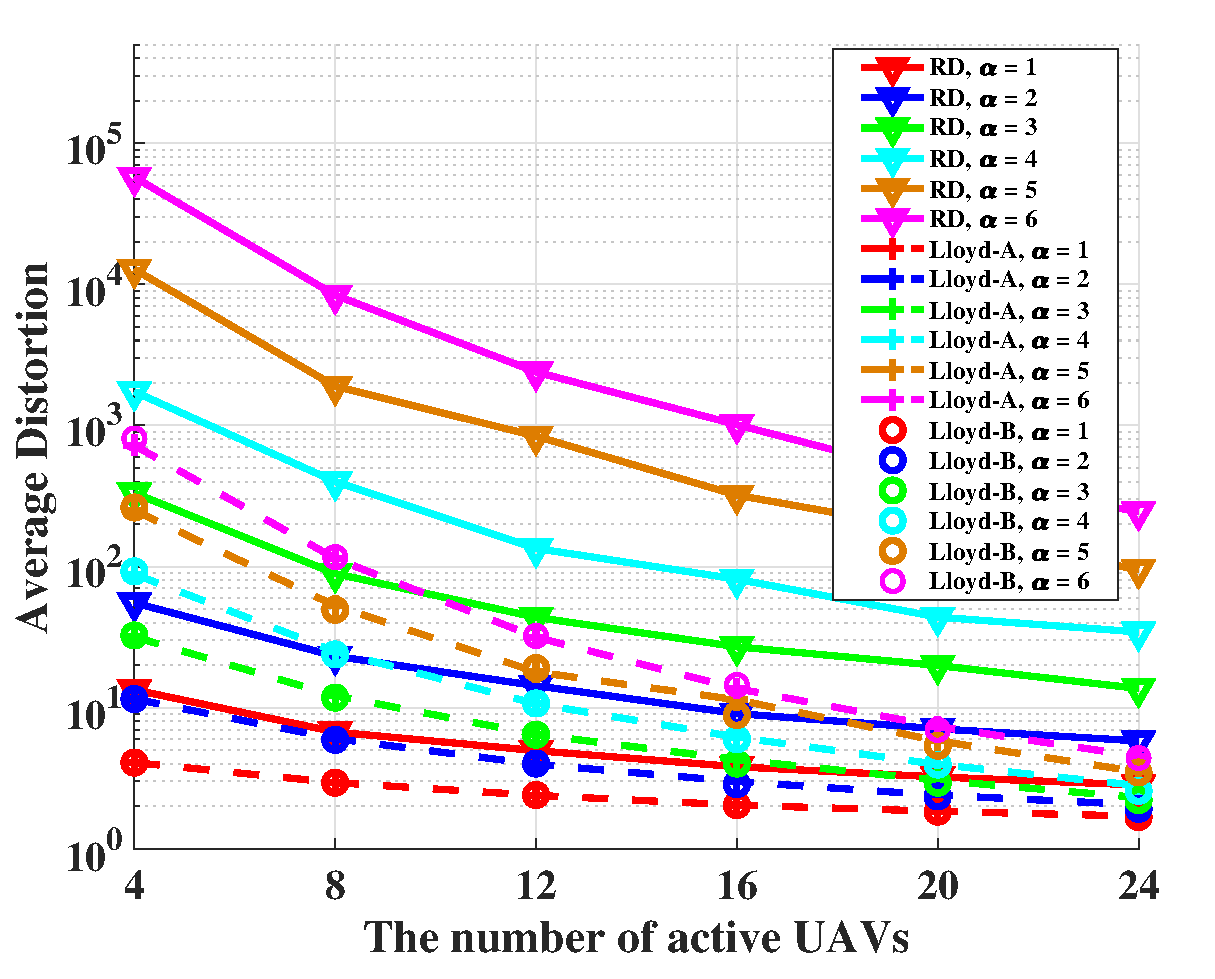
\includegraphics[width=2.9in]{DistortionComparsionUniform.eps}
\label{uniformDistortion}}
\hfil
\subfloat[]{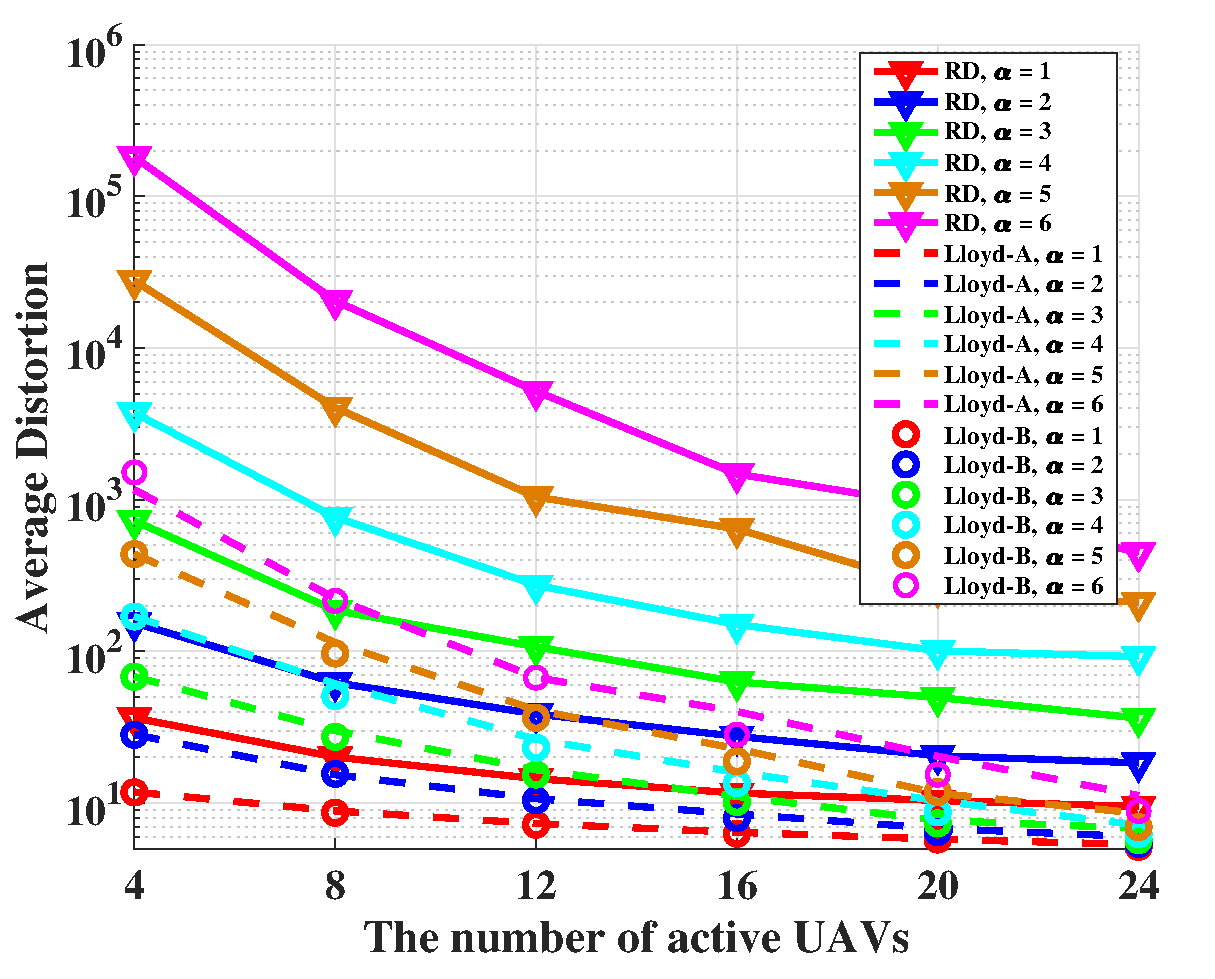
\includegraphics[width=2.9in]{DistortionComparsionNonUniform.eps}
\label{nonuniformDistortion}}
\captionsetup{justification=justified}
\caption{\small{The performance comparison of Lloyd-A, Lloyd-B and Random Deployment (RD). 
(a) Uniform density. (b) Non-uniform density.}}
\label{Distortion}
\end{figure}

To evaluate the performance of the proposed algorithms, we compare them with the average distortion of 100 random
deployments (RD).  Figs. \ref{uniformDistortion} and \ref{nonuniformDistortion}, show that the proposed algorithms
outperform the random deployment on both uniform and non-uniform distributed target regions.  From
\figref{uniformDistortion}, one can also find that the distortion achieved by Lloyd-A and Loyd-B are very close,
indicating that the optimality of the common height, as proved for the one-dimensional case in \secref{sec:optmize1D},
might be extended to the two-dimensional case when the density function is uniform. However, one can find a non-negligible
gap between Lloyd-A and Lloyd-B in \figref{nonuniformDistortion} where the density function is non-uniform. For
instance, given $16$ UAVs and pass loss exponent $\alpha=6$, Lloyd-A's distortion is $40.17$ while Lloyd-B obtains a smaller
distortion, $28.25$, by placing UAVs at different heights.  
%
Figs. \ref{uniformPartitions32} and
\ref{uniformPartitions100} illustrate the UAV ground projections and their partitions on a uniform distributed
square region. As the number of UAVs increases, the UAV partitions approximate to be hexagons which implies the optimality of congruent partition (Theorem \ref{thm:commonheight}) might be extended to uniformly distributed users in two-dimensional sources. 
\ifarxiv However, the UAV projections in Figs. \ref{nonuniformPartitions32} and
\ref{nonuniformPartitions100} show that congruent partition is no longer a necessary condition for the optimal quantizer
when distribution is non-uniform. \else   
However, our
simulations in \cite{GWJ18b} show that congruent partition is no longer a necessary condition for the optimal quantizer
when the source distribution is non-uniform.
\fi
%
\begin{figure}[t]
\centering
\subfloat[]{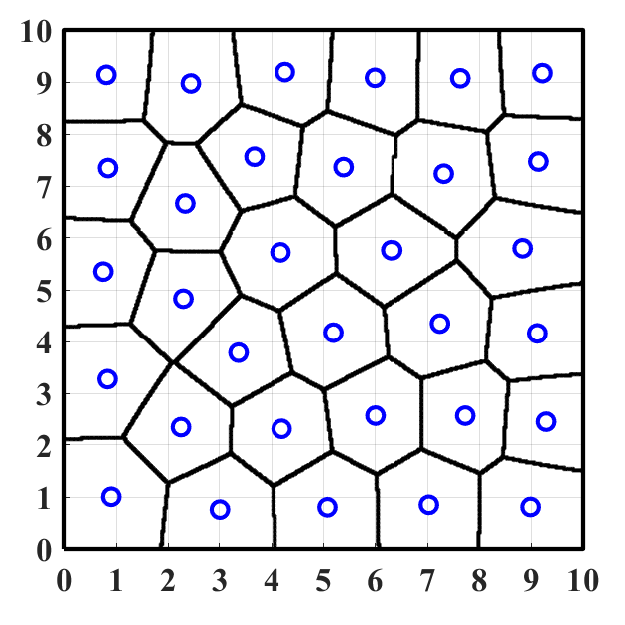
\includegraphics[width=2.8in]{HR32.eps}
\label{uniformPartitions32}}
\hfil
\subfloat[]{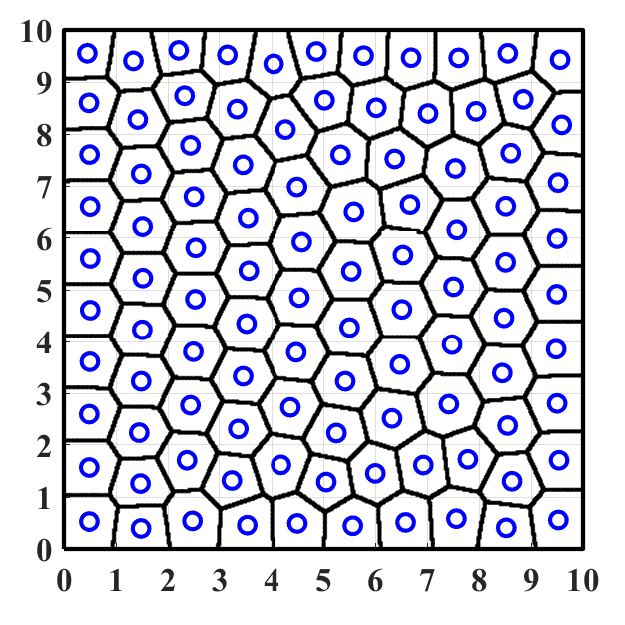
\includegraphics[width=2.8in]{HR100.eps}
\label{uniformPartitions100}}
\captionsetup{justification=justified}
\vspace{-2ex}
\caption{\small{The UAV projections on the ground with generalized Voronoi Diagrams where $\alpha=2$ and the source distribution is uniform. 
(a) 32 UAVs. (b) 100 UAVs.}}
\label{uniformDistortionPartition2}
%\vspace{-4ex}
\end{figure}
\ifarxiv
\begin{figure}[t]
\centering
\subfloat[]{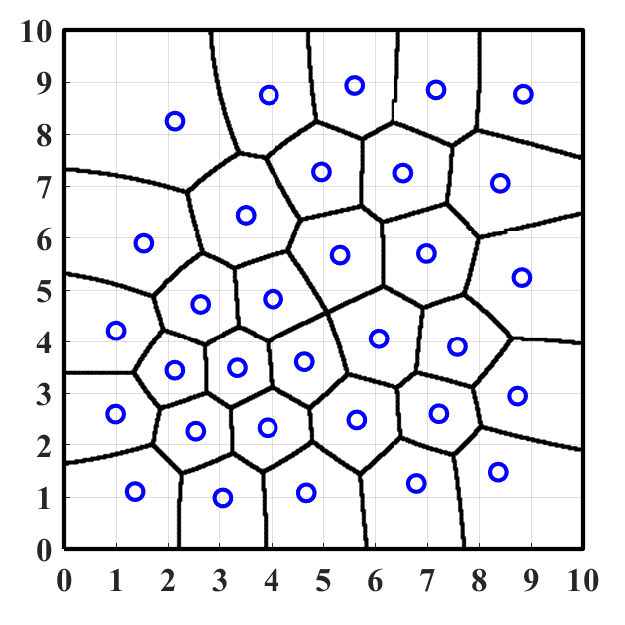
\includegraphics[width=2.8in]{HR32nonUniform.eps}
\label{nonuniformPartitions32}}
\hfil
\subfloat[]{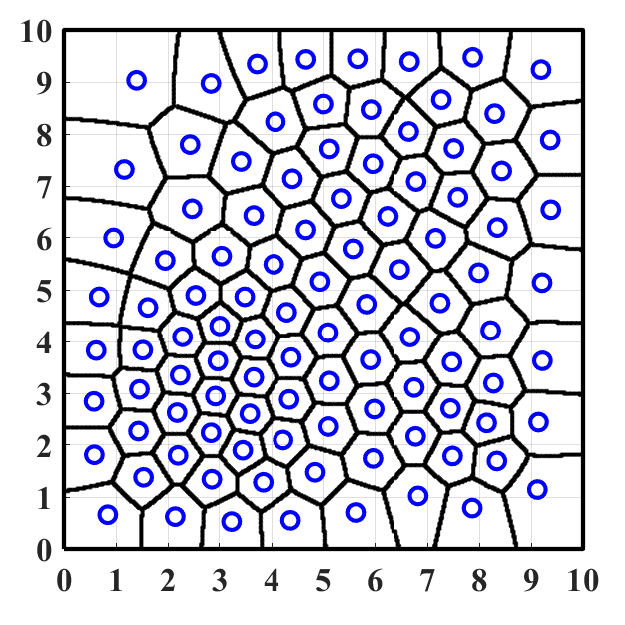
\includegraphics[width=2.8in]{HR100nonUniform.eps}
\label{nonuniformPartitions100}}
\captionsetup{justification=justified}
\vspace{-2ex}
\caption{\small{The UAV projections on the ground with generalized Voronoi Diagrams where $\alpha=2$ and the source distribution is non-uniform. 
(a) 32 UAVs. (b) 100 UAVs.}}
\label{uniformDistortionPartition3}
%\vspace{-4ex}
\end{figure}
\else   \fi
\section{Conclusion}
%
We studied a quantizer with parameterized distortion measure with application in UAV deployment.
Instead of using the traditional mean
distance square as the distortion, we introduce a distortion function which models the energy consumption of UAVs in
dependence of their heights.  We derived the unique parameter optimized quantizer - a uniform scalar quantizer with an
optimal common weight - for uniform source density in one-dimensional space.  In addition, two Lloyd-like algorithms are
designed to minimize the distortion in two-dimensional space.  Numerical simulations demonstrate that for a uniform
density the common weight property extends to two-dimensional space.

\if0 % to much. Only put in here simulations, no analytic example.
In what follows, we provide an example to compare the best deployment with common flight height and an alternative
deployment with different flight heights.  Consider two UAVs over a one-dimensional ground $[0,1]$ with path loss
parameter $\gamma=1$ and a non-uniform density function 
%
\begin{align}
    \lambda(\ome) = 
    \begin{cases}
        4 & \text{if } 0\le\ome\le0.2\\
        \frac{1}{4} & \text{if } 0.2<\ome\le1\\
        0 & otherwise
    \end{cases}
\end{align}
%
Let $q_1=\left(p_1, h_1\right)$ and $q_2=\left(p_2, h_2\right)$ be the deployment of UAV 1 and 2.  First, we derive the
best deployment with common flight height assumption, i.e., $h_1=h_2=h$.  Since the common flight height, the
generalized Voronoi partition is degenerated to Voronoi partition, $V_n(p. h)=\{\ome|\|\ome-p_n\|\le\|\ome-p_m\|,
\forall m\ne n\}$.  Without loss of generality, we assume $0<p_1<p_2<1$, and thus the Voronoi partition can be
represented as $V_1(p, h) = [0, b]$ and $V_2(p, h) = [b, 1]$, where the boundary is 
%
\begin{align}
  b = \frac{p_1+p_2}{2}.\label{boundary}
\end{align}
%
(i) If $b\le0.2$, the distortions can be rewritten as
$D(p,h)=4\int_{0}^{b}\frac{(p_1-\ome)^2+h^2}{h}+4\int_{b}^{0.2}\frac{(p_2-\ome)^2+h^2}{h} +
\frac{1}{4}\int_{0.2}^{1}\frac{(p_2-\ome)^2+h^2}{h}$.  The best deployment satisfies zero-gradient, i.e.,
%
\begin{align}
    &\frac{\partial D}{\partial p_1} = 4\int_{0}^{b}2\frac{(p_1-\ome)}{h}d\ome=0 \label{dp1a}\\
    &\frac{\partial D}{\partial p_2} = 4\int_{b}^{0.2}2\frac{(p_2-\ome)}{h}d\ome
    + \frac{1}{4}\int_{0.2}^{1}2\frac{(p_2-\ome)}{h}d\ome = 0\label{dp2a}\\
    &\frac{\partial D}{\partial h} = 4\int_{0}^{b}\frac{h^2\!-\!(p_1\!-\!\ome)^2}{h^2}d\ome 
    + 4\int_{b}^{0.2}\frac{h^2\!-\!(p_2\!-\!\ome)^2}{h^2}d\ome 
    + \frac{1}{4}\int_{0.2}^1\frac{h^2\!-\!(p_2\!-\!\ome)^2}{h^2}d\ome= 0\notag
\end{align}
Solving (\ref{boundary}), (\ref{dp1a}), and (\ref{dp2a}), we get a quadratic function $8b^2-3b+0.4=0$ which has no real root.
Therefore, $b\le0.2$ is not feasible.\\
(ii) If $b>0.2$, the distortions can be rewritten as
$D(p,h)=4\int_{0}^{0.2}\frac{(p_1-\ome)^2+h^2}{h}+\frac{1}{4}\int_{0.2}^{b}\frac{(p_1-\ome)^2+h^2}{h} + \frac{1}{4}\int_{b}^{1}\frac{(p_2-\ome)^2+h^2}{h}$. 
The best deployment satisfies zero-gradient, i.e.,
\begin{align}
    &\frac{\partial D}{\partial p_1} = 4\int_{0}^{0.2}2\frac{(p_1-\ome)}{h}d\ome
    \frac{1}{4}\int_{0.2}^{b}2\frac{(p_1-\ome)}{h}d\ome=0 \label{dp1b}\\
    &\frac{\partial D}{\partial p_2} = 4\int_{b}^{1}2\frac{(p_2-\ome)}{h}d\ome=0\label{dp2b}\\
    &\frac{\partial D}{\partial h} = 4\int_{0}^{0.2}\frac{h^2\!-\!(p_1\!-\!\ome)^2}{h^2}d\ome 
    + \frac{1}{4}\int_{0.2}^{b}\frac{h^2\!-\!(p_1\!-\!\ome)^2}{h^2}d\ome 
    + \frac{1}{4}\int_{b}^1\frac{h^2\!-\!(p_2\!-\!\ome)^2}{h^2}d\ome= 0\label{dhb}
\end{align}
%
Solving (\ref{boundary}), (\ref{dp1b}), (\ref{dp2b}), and (\ref{dhb}), we get $p^*_1=\frac{3\sqrt{5.8}-7}{2}$,
$p^*_2=\frac{\sqrt{5.8}-1}{2}$, and $h^*=0.096$.  Hence, the minimum distortion with the common flight height is $D(p^*,
h^*)=0.247$.  Next, let $\widetilde{p}=p^*=(p^{*}_1,p^*_2)$ and $\widetilde{h}=(0.05,0.2)$ be an alternative deployment.
By straightforward calculation, we get the corresponding distortion $D(\widetilde{p},\widetilde{h})=0.192$ which is
smaller than that of $D(p^*, h^*)$.  In sum, the common flight height is not a necessary condition for the optimal
deployment.  According to our simulations, there is a big performance gap between the "optimal" deployment with common
flight height and the real optimal deployment.  

\fi % end too much, jun
\if0
Let us further assume that
$\Omega$ is composed on a finite union of intervals  (open or closed does not matter).  Let us further assume all UAVs
have the same flight heights, i.e., $h=h_n$  for all $n=1,2,\dots,N$.  Then each  Möbius region $\Vor_n$ is by
\lemref{lem:moebiusdia} an intersection of half-planes and $\Omega$ and therefore a finite union of intervals
$\Vor_n=\cup_{m=1}^M [a_{n,m},b_{n,m}]$.  

From this characterization we can minimize the communication power function ($\bet=1$) with \lemref{lem:moebiusdia} with
$\Ome=[0,1]$
%
\begin{align}
  \min_{\bP\in[0,1]^N,h>0} \Pbar(\bP,h)= \min_{\bP,h} \sum_{n=1}^N \int_{\Vor_n(\bP)}
  \frac{(\Norm{x_n-\ome}^2 + h^2)^\gam}{h}  d\ome
\end{align}
%
where the Voronoi regions are not anymore dependent on $h$. For $\alp=1$ this simplifies to
%
\begin{align}
  \Pbar_n(\bP,h)=  \frac{1}{h}\int_{\Vor_n}( (\ome-x_n)^2+h^2) d\ome = \frac{1}{h} \int_{\Vor_n} (\ome-p_n)^2
  d\ome + h\int_{\Vor_n} d\ome.
\end{align}
%
By taking the sum over the regions we get
%
\begin{align}
  \Pbar(\bP,h)= \frac{1}{h} \underbrace{\sum_n\int_{\Vor_n} (\ome-x_n)^2 d\ome}_{=H_V(\bP)=H(\bP,V(\bP))} + h
  \label{eq:dph}.
\end{align}
%
Hence, an optimization over $\bP\subset\Omega^N$ only involves the planar Voronoi (power) diagram. A \emph{local minimum} is
attained if the generator points are centroids of there regions \cite{DFG99},\cite{CMKB02}, since it holds
%
\begin{align}
  \nabla H_V(\vP) = \zero &\LRA \forall n \colon 0= \frac{\partial H_V}{\partial x_n} (\vP)=\int_{V_n}
  \frac{\partial}{\partial x_n} (p_n-\ome)^2 d\ome = \int_{V_n} 2(p_n-\ome) d\ome \\
  &\LRA \forall n\colon x_n^*=c_n=\frac{ \int_{V_n} \ome d\ome}{\int_{V_n} d\ome}
\end{align}
%
However, there are infinitely many centroidal Voronoi tessellations $V(\vP^*)$ for $\Omega$, each yielding to a different local
minima $H_V(\vP^*)$. The optimal height $h^*$ for $\vP^*$ is then given by 
\eqref{eq:dph}
%
\begin{align}
  \frac{\partial D(\vP^*,h)}{\partial h} = -\frac{1}{h^{2}} \frac{H_V(\vP*)}{\mu(\Ome)} + 1=0\quad \RA\quad   h^* =
  \sqrt{\frac{H_V(\vP^*)}{\mu(\Ome)}}
\end{align}
%
Let us denote the global minimum by $\hat{H}_V$, then $\hh$ will be the smallest for all centroidal
Voronoi tessellations  $H_V(\vP^*)$. 
For this simple one-dimensional case, we can actually derive the optimal UAV deployment for any $N$.
\fi
%%%%%%%%%%%% old redundant
%  

%
\if0 % not really helpful since no closed form for $h$ can be derived if $\gam>7$
By further substituting with $t=x^2+h^2$ we get
%
\begin{align}
  0&=\frac{1}{2}\int_{h^2}^{(A/2N)^2 + h^2} \frac{t^{\gam}}{\sqrt{t-h^2}} dt - \frac{1}{2}\int_{h^2}^{(A/2N)^2 + h^2}\frac{t^{\gam-1}
(\alp+1)h^2}{\sqrt{t-h^2}} dt\\
0&=\int \frac{t^{\gam}}{\sqrt{t-h^2}} dt - (\alp+1)h^2\int \frac{t^{\gam-1} }{\sqrt{t-h^2}} dt
\end{align}
%
By using integral tables, we can calculate both integrals for any integer $\gam$, i.e., for any odd integer
$\alp\geq 1$, by using \cite[2.241.2.]{GR07b} for $z=x-h^2$ and $t=x$ we get 
%
\begin{align}
  \int \frac{t^n}{\sqrt{z}}dt = 2\sqrt{z} \sum_{k=0}^n \binom{n}{k} \sum_{l=0}^k (-1)^l \binom{k}{l} \frac{z^{k-l}
  (-h^2)^{l}}{2k-2l+1}
\end{align}
%
which gives for $n=\gam$ and $n=\gam-1$
%
\begin{align}
  \sqrt{z}\sum_{k=0}^{\gam} \binom{\gam}{k} \sum_{l=0}^k (-1)^l \binom{k}{l} \frac{z^{k-l}
  (-h^2)^{l}}{2k-2l+1} = \sqrt{z}(\alp+1)h^2
  \sum_{k=0}^{\gam-1} \binom{\gam-1}{k} \sum_{l=0}^k (-1)^l \binom{k}{l} \frac{z^{k-l}(-h^2)^{l}}{2k-2l+1}\notag
\end{align}
%
Using Pascal identity for the binomial coefficients and $(-1)^l (-h^2)^{l}=h^{2l}$
%
\begin{align}
&  \sum_{l=0}^{\gam} \binom{\gam}{l} \frac{z^{\gam-l+0.5}h^{2l}}{2\gam-2l+1} 
+\gam  \frac{z^{0+1/2} (h^2)^{0}}{1}
+\sum_{k=1}^{\gam-1} \binom{\gam-1}{k-1} \sum_{l=0}^k  \binom{k}{l} \frac{z^{k-l+1/2}h^{2l}}{2k-2l+1}\\
&\quad =((\alp+1)h^2-1)
\sum_{k=0}^{\gam-1} \binom{\gam-1}{k} \sum_{l=0}^k  \binom{k}{l} \frac{z^{k-l+0.5}h^{2l}}{2k-2l+1}
\end{align}
%
which simplifies to
%
\begin{align}
   \frac{-\gam A}{2N}&= \Bigg[\sum_{l=0}^{\gam} \binom{\gam}{l} \frac{z^{\gam-l+0.5} h^{2l} }{2(\gam-l)+1} 
  +\sum_{k=1}^{\gam-1} \binom{\gam-1}{k-1} \sum_{l=0}^k  \binom{k}{l} \frac{z^{k-l+0.5} h^{2l}}{2(k-l)+1}\\
 &\quad +(1-(\alp+1)h^2) \sum_{k=0}^{\gam-1} \binom{\gam-1}{k} \sum_{l=0}^k  \binom{k}{l}
 \frac{z^{k-l+0.5}h^{2l}}{2(k-l)+1}\Bigg]_{h^2}^{(A/2N)^2+h^2}
\end{align}
%
\fi % not worth it  i think
%


%\input{LocalOptimization}

\if0 % not relevant anymore, Philipp old stuff
\subsection{Optimal Deployment for different heights of $N=2$ UAVs in one-dimension and $\alp=1$}

Let us consider the case $N=2$ and assume $h_1<h_2$. Then the Moebius regions are
%
\begin{align}
  \Vor_{1}= \Omega\cap B(c_{12},r_{12})\quad,\quad \Vor_{2} = \Omega\cap \Vor_1^c.
\end{align}
%
We ask, if for a uniform density the global minimum is attained if and only if $h_1=h_2=h^*$, where $h^*$ is the global
minimum for constant heights.
In the one-dimensional case the balls are compact intervals, if $\Omega$ is convex, i.e., $\Ome=[0,A]$ w.l.o.g.
The problem has some symmetry, so we can assume $p_1\leq p_2$. If $p_2>p_1$ we can relabel and obtain $h_1>h_2,
p_1<p_2$, which is the scenario where $V_{12}$ is the complement of a ball, so we would just exchange the integral
domains. Hence we only consider the case $p_1\leq p_2, h_1\leq h_2$.
%
We introduce $\eps,\del>0$ to reformulate to
%
\begin{align}
  p_2=p_1+\del, h_2=h_1+\eps, p_1=p, h_1=h\label{eq:phepsdel}
\end{align}
%
We get for the center and radius \eqref{eq:rnmcnm} with \eqref{eq:phepsdel} 
%
\begin{align}
  \begin{split}
  c_{12}&=\frac{h_2 p_1-h_{1}p_2}{h_2-h_1} = p -\frac{\del}{\eps} h\\
  r_{12}&=\sqrt{ \frac{h_1h_2}{(h_2-h_1)^2}(p_1-p_2)^2-h_1^2}
  =\frac{\del}{\eps} h\sqrt{1+\frac{\eps}{h} - \frac{\eps^2}{\del^2}} 
  \end{split}\label{eq:cr}
\end{align}
%
The radius will be always positive, but the center not.
The two Voronoi cells 
%
\begin{align}
  \Vor_1=[0,r_{12}+c_{12}]\quad,\quad \Vor_2=[r_{12}+c_{12},A]
\end{align}
%
have an intersection by \eqref{eq:cr} at
%
\begin{align}
  \td=r_{12}+c_{12}=\frac{h\del}{\eps} (\sqrt{1+\frac{\eps}{h} - \frac{\eps^2}{\del^2}}-1) +p=s(h,\del,\eps) +p
\end{align}
%
which is locally continuous in $\eps$ for $1+\eps/h-\eps^2/\del^2>0$, i.e., $s$ is continuous in $\eps$. More precisely, we can derive the
limit by l'Hopital's rule as
%
\begin{align}
  \lim_{\eps\to 0} s(\eps)=\lim \frac{f(\eps)}{g(\eps)} = \lim \frac{f'(\eps)}{g'(\eps)} =\lim
  \frac{\frac{h\del}{2}(1+\frac{\eps}{h} - \frac{\eps^2}{\del^2})^{-\frac{1}{2}}( h^{-1} -2\eps\del^{-2})}{1}
  =\frac{\del}{2}
\end{align}
%
Hence $\lim_{\eps\to 0}\td(\eps)= p + \del/2$. Indeed, this is independent of $h$ and defines the middle point between
the ground positions $p$ and $p+\del$, assuming both are contained in $[0,A]$, a constrain we need later to impose on
the local minima. 
%
However, if the center dominates the radius, then the distance is negative, but $\td$ is only allowed between $[0,A]$.
If it is outside we need to set it either to $0$ or $A$ (intersection with $\Ome$), i.e.,  
%
\begin{align}
  d=\begin{cases} 
    0   &, \td<0\\
    A   &, \td>A\\
    \td_1 &, \text{else}
  \end{cases}.
\end{align}
%
Without restriction let us set $A=1$ and $\lam$ be uniform, 
then we obtain the objective function
%
\begin{align}
  \Pbar(p,h,\del,\eps) &= \int_{0}^{d} (h^{-1}( p -\ome)^2 + h)d\ome + \int_{d}^1( (h+\eps)^{-1}(p+\del-\ome)^2 +h+\eps) d\ome\\
  &= h+\eps(1-d)+ \frac{1}{h}\int_{0}^{d} ( p -\ome)^2 d\ome + \frac{1}{h+\eps}\int_{d}^1 (p+\del-\ome)^2  d\ome \\
  &= h+\eps(1-d) - \frac{1}{3h}( p -\ome)^3 \Big|_{0}^{d} - \frac{1}{3(h+\eps)}(p+\del-\ome)^3 \Big|_{d}^1\\
  &= h+\eps(1-d)  - \frac{-3p^2 d + 3p d^2 -d^3}{3h} - \frac{(p+\del-1)^3-(p+\del-d)^3}{3(h+\eps)} \\
  &= h+\eps(1-d)  + \frac{3p^2 d - 3p d^2 +d^3}{3h} + \frac{(p+\del-d)^3 -(p+\del-1)^3}{3(h+\eps)} \end{align}
%
\if0
Then 
%
\begin{align*}
 f&=\frac{ 
  (d^3 \!-\!3pd^2 \!+\! 2p^2d)}{h} 
  + \frac{3p^2(1\!-\!d) +3p(\del\!-\!d)^2-3p(\del\!-\!1)^2+(\del\!-\!d)^3 +(1\!-\!\del)^3 +3\del-3\del d}{h+\eps}\\
  &=\frac{(h\!+\!\eps)(d^3 \!-\!3pd^2 \!+\! 2p^2d)}{h(h+\eps)} 
  + \frac{3p^2(1\!-\!d) \!+\! 6p\del(1\!-\!d)+3pd^2\!-\!3p\! + 1\!-\!3\del^2 d\! +\!3\del d \!-\!d^3-3\del+3\del^2\!
  +\!3\del\!-\!3\del d}{h+\eps}\\
  &=\frac{(\eps\!+\!h)(d^3 \!-\!3pd^2 \!+\! 2p^2d)}{h(h+\eps)} 
  + \frac{h(3p^2(1\!-\!d) \!+\! 6p\del(1\!-\!d)+3pd^2\! -3p +1- \!3\del^2 d\! -\!d^3+3\del^2)}{h(h+\eps)}\\
  &=\frac{\eps(d^3 \!-\!3 pd^2 \!+\! 2p^2d )\!+\! hd^3 \!-\!3hpd^2 \!+\! 2hp^2d \!
    -\!3hp^2d  \!+\!3hpd^2\! -\!hd^3 
    +h(3p^2\!+\!6p\del(1\!-\!d)\!-\!3p\!+\!1\!-\!3\del^2 d\! +\!3\del^3)
  }{h(h+\eps)}\\
  &=\frac{\eps(d^3 \!-\!3 pd^2 \!+\! 2p^2d) \!
    -\! hp^2d\!
    +h(3p^2\!+\!6p\del(1\!-\!d)\!-\!3p\!+\!1\!-\!3\del^2 d\! +\!3\del^3)
  }{h(h+\eps)}\\
  &=\frac{\eps h^{-1}( d^3 \!-\!3 pd^2 \!+\! 2 p^2d )
    \!-\!p^2d\!+\! 3p^2  \!-\!6p\del d\!+\!6p\del\! -\!3p\! 
  +1 -3\del^2 d +3\del^2
  }{h+\eps}\\
  &=\frac{\frac{\eps}{h}( (s+p)^3 \!-\!3 p(s+p)^2 \!+\! 2 p^2s + 2p^3 \!)
      \!-s(6p\del+3\del^2+ p^2) +\! 3p^2\! - p^3 - 6p^2\del\!+\!3p\del\! -\!3p\! 
  +1  +3\del^2
  }{h+\eps}
\end{align*}
%
We can take the derivative after $p$, which is only in the numerator present
%
\begin{align} 
  f'(p)&=\frac{ \frac{\eps}{h}\Big[3(s+p)^2-3(s+p)^2-6p(s+p) +4ps +6p^2\Big] +6p -2ps-3p^2-6\del s
-12p\del +3\del -3 }{h+\eps}\\
\RA \quad& f'(p^*)=0\\
\RA \quad& p(2s-6+3p+12\del) +6\del s -3\del +3  = p\eps h^{-1}(-6(s+p)+4s+6p)\\
\LRA \quad& p(2s-6+3p+12\del +2s\eps h^{-1}) +6\del s -3\del +3 = 0\\
\LRA \quad& p^2 + p\underbrace{\frac{2s-6+12\del +2s\eps h^{-1}}{3}}_{=a} + \underbrace{2\del s -\del +1 }_{=b}=0
\end{align}
%
This gives two solutions for $p$
%
\begin{align}
  p^*_{1,2}= 
  -\frac{s-3+6\del +s\eps h^{-1} \pm \sqrt{(s-3+6\del +s\eps h^{-1})^2 -18\del s +9\del -9 }}{3}
\end{align}

\fi



Numerically simulations, suggest that the optimal minimum is attained for common flight heights, see
\figref{fig:globalnum_fixheight} for $N=2$ by optimizing over $\eps$ and $p=p_1$ for fixed $\del=0.5$.
Indeed, the optimum is attained for the blue plot with $h=h_1=0.144$ at $\eps=0$, i.e., $h_2=h_1=h$ as derived in
\thmref{thm:onedimglobalmin}. 

\begin{figure}[t]
  \centering
\subfloat[]{
 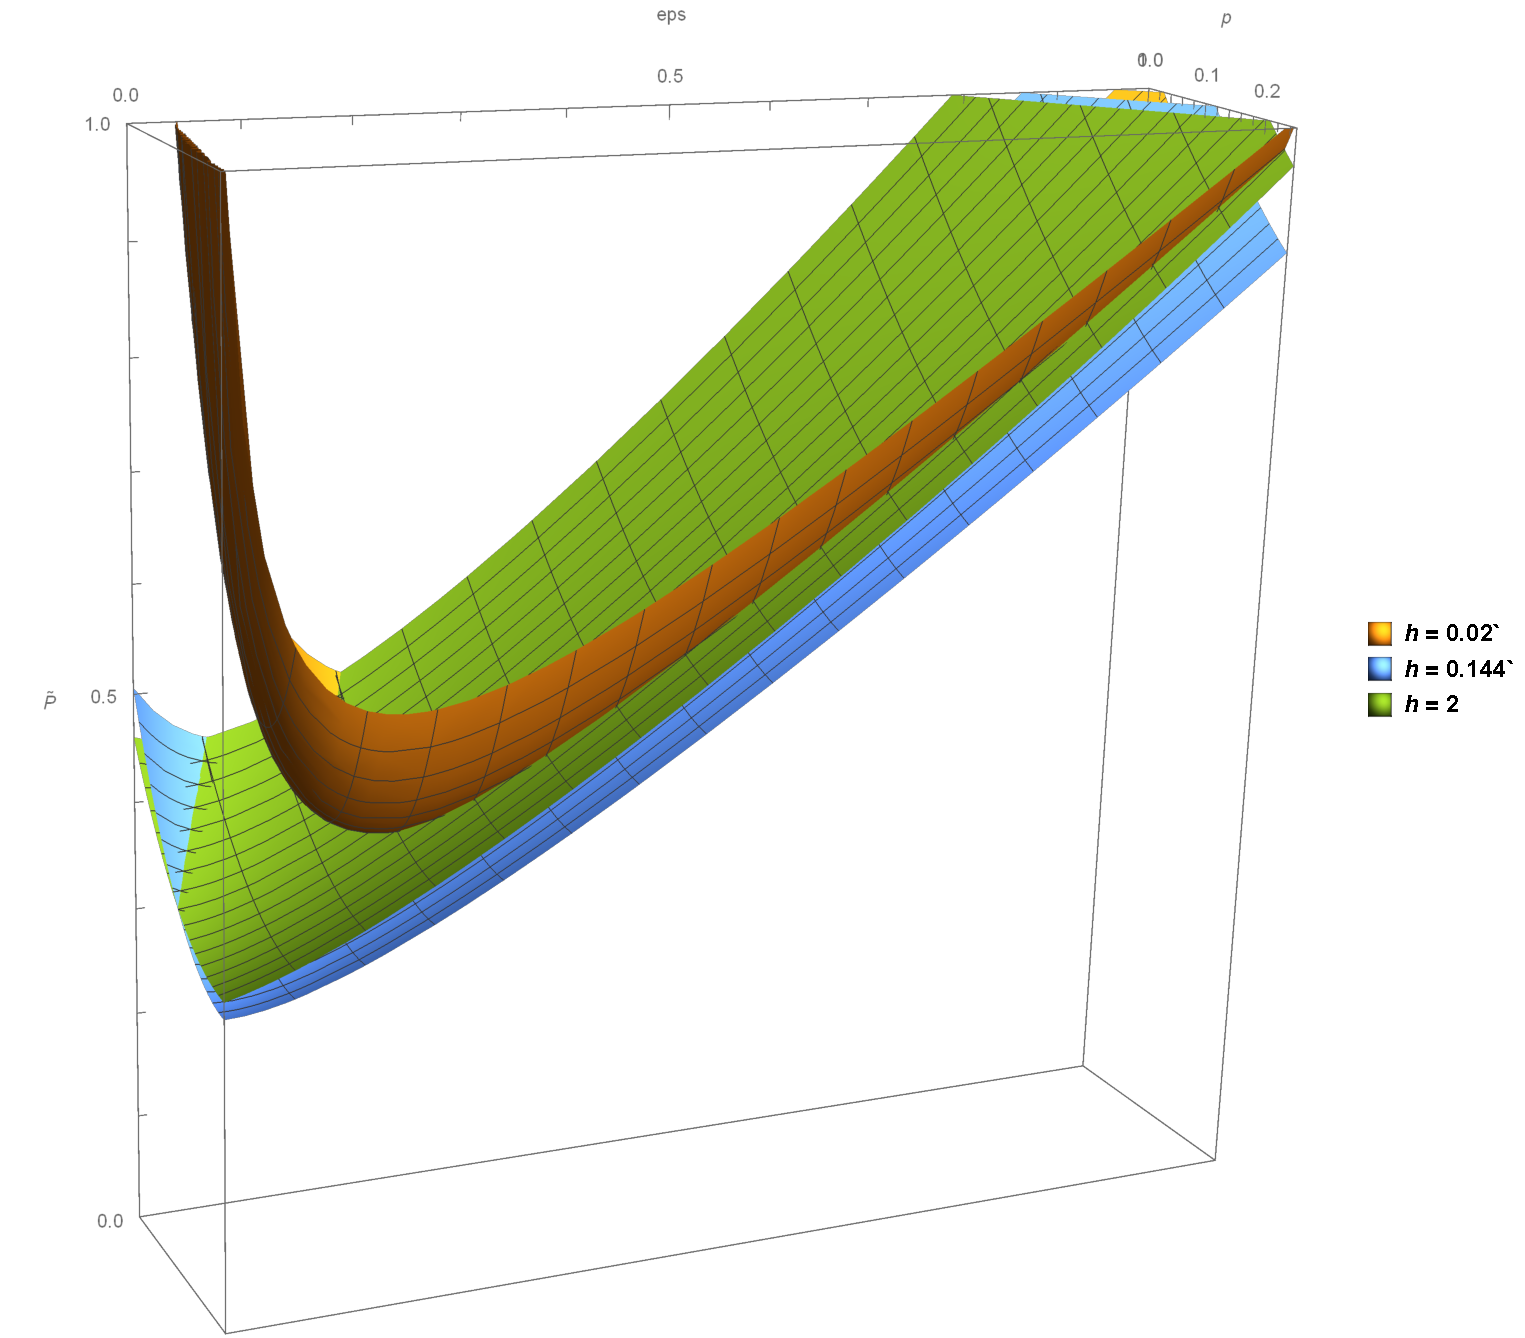
\includegraphics[width=0.9\textwidth]{Pepsandpone.pdf}
 \label{1b}\hfill}
%\subcaption{$h_1=0.144,h_2=0.6$}
 \caption{Global minima for fixed $\del=0.5$ and three heights $h=h_1$  over  $\eps\in[0,1]$ and $p=p_1\in[0,0.25]$.
   For $h=h_1=0.144$ the blue plot achieves the ``global'' minimum at $\eps=0$ and $p_1=0.25$. Note, that the brown curve
 not achiev its local minimum for same heights, since $\eps\sim0.15$.}\label{fig:globalnum_fixheight}
\end{figure}


\fi

\color{black}




\ifarxiv
\appendices
\section{Proof of \lemref{lem:ggam}}\label{app:proof_lemma_ggam}
  To find the optimal $1-$level parameter quantizer $(x^*,h^*)$ for a uniform density $\lam(\ome)=1/A$, we need to
  satisfy \eqref{eq:criticalpoint}, i.e., for\footnote{Note, there is no optimizing over the regions, since there is only
  one.} $\Ome=\Vor_1=\Vor_1^*=[0,A]$
  %
  \begin{align}
    0&=\int_0^A (x^*-\ome)\big( (x^*-\ome)^2+h^{*2}\big)^{\gam-1}  d\ome.
  \end{align}
  %
  Substituting $x^*-\ome$ by $\ome$ we get 
  %
  \begin{align}
    0&=\int_{x^*-A}^{x^*} \ome \big( \ome^2+h^{*2}\big)^{\gam-1}  d\ome
  \end{align}
  %
  Since the integral kernel is an odd function in $\ome$ and $x^*\in[0,A]$, it must hold
  %
  \begin{align}
    0=-\int_0^{x^*-A} \ome(\ome^2+h^{*2})^{\gam-1}d\ome + \int_0^{x^*}\ome(\ome^2+h^{*2})^{\gam-1}d\ome
    \intertext{by substituting $\ome$ by $-\ome$ we get}
    \int_{0}^{A-x^*} \ome(\ome^2+h^{*2})^{\gam-1}d\ome = \int_0^{x^*} \ome(\ome^2+h^{*2})^{\gam-1}d\ome.
  \end{align}  
  %
  Hence for any choice of $h^*$ it must hold $x^*=A-x^*$, which is equivalent to $x^*=A/2$.
%  We also note at this point, that for setting $x^*=A/2\pm \eps$ for any $\eps>0$, will obtain   
  To find the optimal parameter, we can just insert $x^*$ into the average distortion
  %
  \begin{align}
    \AvDis(x^*,h) &= \frac{1}{A}\int_0^A \frac{(x^*-\ome)^2+h^2)^{\gam} }{h}d\ome
    = \frac{1}{A} \int_0^{A/2} \frac{(\ome^2+h^2)^{\gam}}{h}d\ome\label{eq:AvDisxstar}
  \intertext{where we substituted again and inserted $x^*=A/2$. By substituting $\ome$ with $2\ome/A$ 
    and $h$ with $u=2h/A$  we get}
    &= \int_0^1  \frac{2}{A}\frac{((A\ome/2)^2 +   (Au/2)^2)^{\gam}}{u}d\ome
      =\left(\frac{A}{2}\right)^{2\gam-1} \int_0^1 f(\ome,u,\gam)d\ome
  \end{align}
  %
  where for each $\gam\geq 1$ the integral kernel $f$ is a convex function in
  $\vx=(\ome,u)$ over $\R_+^2$. Let us rewrite $f$ as
  %
  \begin{align}
    f(\ome,u,\gam)= \frac{(\ome^2+u^2)^{\gam}}{u}= \frac{\Norm{(\ome,u)}_2^{2\gam}}{u}.
  \end{align}
  %
  Clearly, $\Norm{\vx}_2$ is a convex and continuous function in $\vx$ over $\R^2$ and since $(\cdot)^{2\gam}$ with
  $2\gam\geq2$ is a strictly increasing continuous function, the concatenation $f(\vx,\gam)$ is a strict convex and
  continuous function over $\R_+^2$. Hence, for any $\vx_1,\vx_2\in\R^2$ we have
  %
  \begin{align}
    \Norm{\lam\vx_1+(1-\lam)\vx_2}_2^{2\gam}<\lam \Norm{\vx_1}_2^{2\gam} + (1-\lam)\Norm{\vx_2}_2^{2\gam}
  \end{align}
  %
  for all $\lam\in(0,1)$. But then we have also for any $u_1,u_2\in\R^2_+$ and $\ome\geq 0$ 
  %
  \begin{align}
    f(\lam u_1 +(1-\lam)u_2,\ome,\gam) < 
    \frac{\lam\Norm{(\ome,u_1)}_2^{2\gam} + (1-\lam)\Norm{(\ome,u_2)}_2^{2\gam}}{\lam u_1+(1-\lam)u_2}
    \label{eq:fnormgam}.
  \end{align}
  %
  Considering the following inequality 
  %
  \begin{align}
    \frac{1}{u_1}\! +\!\frac{1}{u_2} &=
       \left(\frac{1}{u_1}\! + \!\frac{1}{u_2}\right)\frac{\lam u_1 \!+\!(1\!-\!\lam)u_2}{\lam u_1 \!+\! (1\!-\!\lam)u_2}
       =\frac{ \left(\lam\! +\!\frac{(1\!-\!\lam)u_2}{u_1}\! +\! (1\!-\!\lam) \!+\! \frac{\lam u_1}{u_2}\right)}{\lam
       u_1 \!+\! (1\!-\!\lam)u_2} 
       > \frac{1}{\lam u_1\! +\! (1\!-\!\lam)u_2}\notag
  \end{align}
  %
  and \eqref{eq:fnormgam}, we will have
  %
  \begin{align}
    f(\lam u_1 +(1-\lam)u_2,\ome,\gam) < \lam f(u_1,\ome,\gam) + (1-\lam)f(u_2,\ome,\gam) 
  \end{align}
  %
  for every $\lam\in(0,1)$. Hence, the integral kernel is strictly convex for every $\ome\geq0,\gam\geq 1$, and since the
  infinite sum (integral) of convex functions is again a convex function, for $u>0$, we have shown convexity of $F(u,\gam)$. 
  Note, $f(u,\ome,\gam)$ is continuous in $\R_+^2$ since it is a product of the continuous functions
  $\Norm{(u,\ome)}_2^{2\gam}$ and $1/(u+0\cdot\ome)$, and so is $F(u,\gam)$. 
  %
  Therefore, the only critical point of $F(\cdot,\gam)$ will be the unique global minimizer
  \begin{align}
    g(\gam)=\arg\min_{u>0} F(u,\gam),
  \end{align}
  %
  which is defined by the  vanishing of the first derivative:
  %
  \begin{align}
    F'(u)  &\!= \!\int_0^{1}\! (\ome^2\!+\!u^2)^{\gam-1} \left( (2\gam\!-\!1)-\frac{\ome^2}{u^2}\right)d\ome
    \!=\!\frac{1}{u^{2}}\!\int_{0}^{1} (\ome^2\!+\!u^2)^{\gam-1}\left((2\gam\!-\!1)u^2-\ome^2\right)d\ome\label{eq:Fderivative}.
  \end{align}
  %
  Hence, $F'(u)$ can only vanish if $u<1/\sqrt{2\gam-1}$, which is an upper bound on $g(\gam)$.
  The optimal parameter for minimizing the average distortion  \eqref{eq:AvDisxstar} is then 
  %
  \begin{align}
    h^*= \frac{A}{2} g(\gam) \quad\text{with}\quad \AvDis(x^*,h^*)= \left(\frac{A}{2}\right)^{2\gam-1} g(\gam).
  \end{align}
  %
  Analytical solutions for $F'(u)=0$ are possible for integer valued $\gam$.  Let us set $0<x=u^2$ in
  \eqref{eq:Fderivative}, then for $\gam\in\N$, the integrand in \eqref{eq:Fderivative} will be a polynomial in $\ome$
  of degree $2\gam$ and in $x$ of degree $\gam$. For $\gam\in\{1,2,3\}$ the integrand will be 
%
\begin{align}
  (\ome^2+x)^0 (1x-\ome^2)&=x-\ome^2\\
  (\ome^2+x)^1 (3x-\ome^2)&=3x^2+2\ome^2x -\ome^4 \\
  (\ome^2+x)^2 (5x-\ome^2)&=5x^3 +9\ome^2 x^2 +3\ome^4 x -\ome^6
%  (x^2-7c)(x^2+c)^3 &=x^8 -4x^6c -18x^4c^2-20x^2c^3-7c^4
\end{align}
%
which yield with the definite integrals to
%
\begin{align}
  0 &= \ome(x-\frac{\ome^2}{3})\Big|_{\ome=1}\label{eq:xfirst}\\
  0 &= \ome( 3x^2 +\frac{2\ome^2x}{3} -\frac{\ome^4}{5}  )\Big|_{\ome=1}\label{eq:xtwo}\\ 
  0 &= \ome( 5x^3 + 3\ome^2x^2 +\frac{3\ome^4x}{5}  -\frac{\ome^6}{7}  )\Big|_{\ome=1}\label{eq:ccubic} 
%  0 &= x(\frac{x^8}{9} -\frac{4x^6c}{7} - \frac{18x^4c^2}{5} -\frac{20x^2c^3}{3} - 7c^4)\Big|_{x=b}
\end{align}
%
Solving \eqref{eq:xfirst} for $x$  yields to the only feasible solution
%
\begin{align}
  x=\frac{1}{3} \quad\RA\quad g(1)=\frac{1}{\sqrt{3}}\approx 0.577.
\end{align}
%
The solutions of \eqref{eq:xtwo} are 
%
\begin{align}
  x_{1,2}= -\frac{1}{9} \pm \sqrt{\frac{1}{81}+\frac{1}{15}} = \frac{\pm \sqrt{32/5} -1}{9}
\end{align}
%
Since only positive roots are allowed, we get as the only feasible solution
%
\begin{align}
  g(3)=\frac{\sqrt{\sqrt{32/5}-1}}{3}\approx 0.412.
\end{align}
%
Finally, the cubic equation \eqref{eq:ccubic} results in
%
\begin{align}
  5x^3 + 3 x^2 + \frac{3}{5} x - \frac{1}{7}=0
\end{align}
%
The solution of a cubic equation can be found in \cite[2.3.2]{Zwi03} by calculating the discriminant
%
\begin{align}
  \Del=q^2+4p^3 \quad\text{with}\quad q=\frac{2b^3-9abc+27a^2d}{27a^3},p=\frac{3ac-b^2}{9a^2}
\end{align}
%
Let us identify $a=5,b=3,c=3/5$ and $d=-1/7$, then we get
%
\begin{align}
  q&=\frac{6\cdot 9-9\cdot 9 - 27\cdot 5^2\cdot1/7}{27\cdot 5^3}
  =-\frac{3}{3\cdot 5\cdot 25} -\frac{1}{5\cdot 7}=-\frac{32}{25\cdot35}\\
  \Del&=q^2 + 4 \left(\frac{3\cdot 3 -9}{9\cdot 5^2}\right)^3=q^2>0
\end{align}
%
which indicates only one real-valued root, given by
%
\begin{align}
  x=\alp_+^{1/3}+\alp_-^{1/3}-\frac{b}{3a} 
  \quad\text{with}\quad  \alp_{\pm}=\frac{-q\pm\sqrt{\Del}}{2} = \left\{0, \frac{32}{25\cdot 35} \right\}
\end{align}
%
which computes to
%
\begin{align}
  x=\left( \frac{32}{5^3\cdot 7}\right)^{1/3}- \frac{1}{5}
  =\frac{(\frac{32}{7})^{1/3}-1}{5} \RA g(5)=\sqrt{\frac{(\frac{32}{7})^{1/3}-1}{5}} \approx 0.363.
\end{align}
%
\fi % ifarxiv end


\ifarxiv%
%
\section{Proof of \lemref{lemma:allActive}}\label{app:proof_lemma_active}
  %
  Although, this statement seems to be trivial, it is not straight forward to show.
%  , since the distortion function
%  $\AvDis$ in \eqref{eq:Eptx} is not strictly monotone increasing in $p_n$ or $h_n$ for a given sample $\ome \in\Ome$.
%  To bypass this non-monotonicity property  
  We will use the quantization relaxation for the average distortion $\AvDis$
  in \eqref{eq:Pbar} to  show that the $N-$level parameter optimized quantizer has strictly smaller distortion than the
  $(N-1)-$level optimized quantizer \eqref{eq:optPbar}. We define, as in
  quantization theory, see for example \cite{GN98}, an \emph{$N-$level quantizer} for $\Ome$, by a (disjoint) partition
  $\Rset=\{\Rset_n\}_{n=1}^N\subset \Ome$ of $\Ome$ and assign to each partition region $\Rset_n$ a
  parameter-quantization point
  $(\vp_n,h_n)\in\Ome\times\R_+$. The assignment rule or \emph{quantization rule} can be anything such that the regions
  are independent of the value of the parameter and quantization points.  Minimizing over all quantizer, that is, over
  all partitions and possible parameter-quantization points will yield to the parameter optimized quantizer, which is by definition the
  optimal deployment (reproduction points) which generate the generalized Voronoi regions as the optimal partition
  (tessellation\footnote{Since we take here the continuous case, the integral will not distinguish between open or closed
  sets.}). This holds for any density function $\lam(\ome)$ and target area $\Ome$.  To see this\footnote{We use the
    same argumentation as in the prove of \cite[Prop.1]{Erdem}.} let us start with any quantizer $(\vP,\vh,\Rset)$ for
    $\Ome$ yielding to the average distortion 
  %
  \begin{align}
    \AvDis(\vP,\vh,\Rset) &=\sum_{n=1}^N \int_{\Rset_n} \Dis(\vp_n,h_n,\ome)\lam(\ome) d\ome \geq \sum_{n=1}^N \int_{\Rset_n} 
    \left(\min_{m\in[N]} \Dis(\vp_m,h_n,\ome) \right) \lam(\ome)d\ome\notag\\
    &=\int_{\Ome} \min_{m\in[N]} \Dis(\vp_m,h_n,\ome) \lam(\ome)d\ome
    =\sum_n \int_{\Vor_n(\vP,\vh)} \Dis(\vp_n,h_n,\ome) \lam(\ome)d\ome
  \end{align} 
  %
  where the first inequality is only achieved if for any $\ome\in \Rset_n$ we have chosen $(\vp_n,h_n)$ to be the optimal
  quantization point with respect to $\Dis$, or vice versa, if every $(\vp,h_n)$ is optimal for every $\ome\in \Rset_n$, which is the
  definition of the generalized Voronoi region $\Vor(\vP,\vh)$. Therefore, minimizing over all partitions gives equality, i.e.
  %
  \begin{align}
    \min_{\Rset} \AvDis(\vP,\vh,\Rset)=\AvDis(\vP,\vh,\Vor(\vP,\vh))
  \end{align}
  %
  for any $(\vP,\vh)\in\Ome^N\times\R_+^N$.
  Hence, we have shown that the parameter-quantizer optimization problem is equivalent to the locational-parameter
  optimization problem
  %
  \begin{align}
    \min_{\vP\in\Ome^N,\vh\in\R_+^N} \min_{\Rset\in\Ome^N} \AvDis(\vQ,\Rset) 
    = \min_{\vP\in\Ome^N,\vh\in\R_+^N} \AvDis(\vP,\vh,\Vor(\vP,\vh))=\AvDis(\vP^*,\vh^*,\Vor^*).\label{eq:optquanteqoptdeploy2}
  \end{align}
  %
  We need to show, that for the optimal $N-$parameter-quantizer $(\vP^*,\vh^*,\Vor^*)$ with $\Vor^*=\Vor(\vP^*,\vh^*)$
  we have $\mu(\Vor_n)>0$ for all $n\in[N]$.  Let us first show that each region is indeed a closed interval, i.e.,
  $\Vor_n^*=[b^*_{n-1},b^*_n]$ with $0\leq b^*_{n-1}\leq b^*_n\leq A$. 
  
  By the definition of the Möbius regions in \lemref{lem:moebiusdia}, each dominance region is either a single interval
  (if it is a ball not contained in the target region or a halfspace) or two disjoint intervals (if its a ball contained
  in the target region), we can not have more than $K_n\leq 2N-2$ disjoint closed intervals for each Möbius (generalized
  Voronoi) region.  Therefore, the $n$th optimal Möbius region is given as $\Vor^*_n=\bigcup_{k=1}^{K_n}v_{n,k}$, where
  $v_{n,k}=[a_{n,k-1},a_{n,k}]$ are intervals for some $0\leq a_{n,k-1}\leq a_{n,k}\leq A$.

  Let us assume there are quantization points with disconnected regions, i.e. $K_n>1$ for $n\in\Ind_d$ and some
  $\Ind_d\subset[N]$. Then we will re-arrange the partition $\Vor^*$ by concatenating the $K_n$ disconnected
  intervals $v_{n,k}$ to $\Rset_n=[b_{n-1},b_{n}]$ for $n\in\Ind_d$ and move the connected regions appropriate such that
  for all $n\in[N]$ it holds $\mu(\Rset_n)=\mu(\Vor^*_n)=b_n-b_{n-1}$ and $b_{n-1}\leq b_{n}$, where we set $b_0=0$ and
  $b_N=A$. For the new concatenated regions, we move each $q_n^*$ to the center of the new arranged regions, i.e.,
  $\tq_n=\frac{b_n+b_{n-1}}{2}$ for $n\in\Ind_d$. If for the connected regions $n\in[N]\setminus\Ind_d$  the
  quantization points $q^*_n$ are not centroidal, than by placing them in the center of the closed interval,
  will by \lemref{lem:ggam} obtain a strictly smaller distortion. Hence, for the optimal quantizer, the quantization
  points must be centroidal and we can assume $\tq_n=(b_n+b_{n-1})/2$ for all $n\in[N]$. 
  %
  In this rearrangement we did not changed the parameters $h_n^*$ at all.  The so rearranged partition
  $\Rset=\{\Rset_n\}$ and replaced quantization points $\tvp=(\tq_1,\dots,\tq_N)$ has the average distortion 
  %
  \begin{align}
    \AvDis(\tvp,\vh^*,\Rset)=\sum_{n=1}^N \int_{b_{n-1}}^{b_n} \frac{ ((\tq_n\!-\!\ome)^2+h_n^{*2})^{\gam}}{h_n^{*}} d\ome
      = 2\sum_{n=1}^N \int_{0}^{\frac{b_n-b_{n-1}}{2}} \frac{ (\ome^2+h_n^{*2})^{\gam}}{h_n^{*}} d\ome
  \end{align}
  %
  where we substituted $\ome$ by $\tq_n\!-\!\ome$. Since the parameters did not changed and the function
  $(\ome^2+h_n^{*2})^{\gam}$ is strictly monotone increasing in $\ome$ for each $\gam>0$, it holds for the average
  distortion of regions $n\in\Ind_d$
  %
  \begin{align}
   \AvDis_n(\tq_n,h_n^*,\Rset_n)=    2\int_{0}^{\frac{b_n-b_{n-1}}{2}} \frac{ (\ome^2+h_n^{*2})^{\gam}}{h_n^{*}} d\ome 
    < \sum_{k=1}^{K_n}\int_{a_{n,k}-q_n^*}^{a_{n,k-1}-q_n^*} \frac{ (\ome^2+h_n^{*2})^{\gam}}{h_n^{*}}
    d\ome\label{eq:Avdisn}
  \end{align}
  %
  since the non-zero gaps in $\bigcup_k [a_{n,k}-q_n^*,a_{n,k-1}-q_n^*]$ will lead to larger $\ome$ in the RHS integral
  and therefore to a strictly larger average distortion.  Therefore the points $(\tvp,\vh^*)$ with closed interval
  $\Rset=\{\Rset_n\}$ have a strictly smaller average distortion, which contradicts the assumption that $(\vp^*,\vh^*)$ is the
  parameter optimized quantizer \eqref{eq:optquanteqoptdeploy}. Hence $K_n=1$ for each $n\in[N]$ and every $\gam\geq 1$.
  Moreover, the optimal quantization points must be centroids of the intervals, i.e. $x_n^*=(b_n^*+b_{n-1})/2$.

%%%%%%%%%%%%%%%%%%%%%%%%%%%%%%%%%%%%%%%%%%%%%%%%%%%%%%%%%%%%%%%%

  Now, we have to show that the optimal quantization regions $\Vor_n^*=\{[b^*_{n-1},b^*_n]\}_{n=1}^n$ are not points, i.e.,
  it should hold $b^*_n>b^*_{n-1}$ for each $n\in[N]$. If $b^*_n=b^*_{n-1}$ for some $n$, then the $n$th average distortion $\AvDis_n$
  would be zero for this quantization point, since the integral is vanishing. But then we only optimize over $N-1$
  quantization points. So we only need to show, that an additional quantization point strictly decreases the minimal
  average distortion.  Hence, take any non-zero optimal quantization region $\Vor_n^*=[b^*_{n-1},b^*_n]$. We know by
  \lemref{lem:ggam} that the optimal quantizer $q_n^*$ for some closed interval $\Vor_n^*$  must be its centroidal for
  any parameter $h_n$.  Hence, if we split  $\Vor_n^*$ with  $A_n=b^*_n-b^*_{n-1}$ by a half and put two quantizers
  $q_{n_1}$ and $q_{n_2}$ with same parameter $h_n^*$ in the center we will get with \eqref{eq:Avdisn}
  %
  \begin{align}
   % D_n(q_n^*,h_n^*,\Vor_n^*)=\frac{2}{h_n}\int_{0}^{A_n/2} (\ome^2+h_n^{*2})^{\gam} d\ome
      \AvDis_{n_1}\!+\!\AvDis_{n_2}&=\frac{1}{h_n^*} 
     \left( \int_{b_{n-1}}^{b_{n-1}+\frac{A_n}{2}} ( (q_{n_1}-\ome)^2 + h_n^{*2})^{\gam}d\ome
     +\int_{b_{n-1}+\frac{A_n}{2}}^{b_n}((q_{n_2}-\ome)^2+h_n^{*2})^{\gam}d\ome\right)\notag\\
   \intertext{substituting $q_{n_i}-\ome$ by $\ome$ we get} 
     & =  \int_{-\frac{A_n}{4}}^{\frac{A_n}{4}} \frac{(\ome^2+h_n^{*2})^{\gam}}{h_n^*}d\ome
     + \int_{-\frac{A_n}{4}}^{\frac{A_n}{4}} \frac{(\ome^2+h_n^{*2})^{\gam}}{h_n^*}d\ome\\
     & =  2\int_{0}^{\frac{A_n}{4}} \frac{(\ome^2+h_n^{*2})^{\gam}}{h_n^*}d\ome 
     + w\int_{0}^{\frac{A_n}{4}}    \frac{ (\ome^2+h_n^{*2})^{\gam}}{h_n^*}d\ome\\
     & <  2\!\int_{0}^{\frac{A_n}{4}} \frac{(\ome^2\!+\!h_n^{*2})^{\gam}}{h_n^*}d\ome
     + 2\!\int_{\frac{A_n}{4}}^{\frac{A_n}{2}} \frac{(\ome^2\!+\!h_n^{*2})^{\gam}}{h_n^*}d\ome
     = 2\!\int_0^{\frac{A_n}{2}} \frac{(\ome^2\!+\!h_n^{*2})^\gam}{h_n^*} d\ome=\AvDis_n\notag
  \end{align}
  Hence, the average distortion will strictly decrease if $A_n>0$. Therefore, the $N-$level parameter optimized
  quantizer will have
  quantization boundaries $b_n\!>\!b_{n\!-\!1}$ for $n\in[N]$.
  % old version, too complicated
  \if0
  By \eqref{eq:optquanteqoptdeploy} we get 
  %
  \begin{align}
    \min_{\Rset} \Pbar(\vQ^*,\Rset)= \min_{\Rset}\sum_n \int_{\Rset_n} P(\vq^*_n,\vome)d\vome=\Pbar(\vQ^*,\Vor(\vQ^*)).
  \end{align}
  %
  If $N=1$ there is nothing to optimize and we have $\Rset=\Rset_1=\Ome=[a,b]$. Furthermore, we know  by
  \lemref{lem:ggam}, that the optimal $\vq^{(1)*}=(p_1^{(1)*},h_1^{(1)*})$ for $N=1$ is the uniform quantizer given by
  $p^{(1)*}_1=a+A/2$ with $A=b-a$ and $h^*=h_1^{(1)*}=\argmin_{h>0} \int_0^{A/2} \frac{(\ome^2+h^2)^{\gam}}{h}d\ome$.
  Let us note, that the average power $\Pbar(p_1^{(1)*},\cdot)$ is convex (second-derivative is always positive) in $h$
  and hence there is only one critical point $h^*$ in $\R_+$, which is the global minimum. Now assume, we add one more
  quantizer $\vq_2^{(2)}=(p_2^{(2)},h^*)$ with same height and partitioning $\Ome$ by $\Rset_{\eps}$ given by
  $R_1=[a,a+\eps]$ and $R_2=[a+\eps,b]$  for some $\eps\in(0,A)$.  If we minimize only over the ground positions, we get 
  %
  \begin{align}
    \Pbar(\vp^{(2)*},h^*,\Rset_{\eps}):=\min_{p_1} \int_{a}^{a+\eps} P(p_1,h^*,\ome)d\ome + \min_{p_2} 
    \int_{a+\eps}^b P(p_2,h^*,\ome)d\ome
  \end{align}
  %
  By the \lemref{lem:ggam} we get for the optimal uniform ground positions for each {\bfseries independent} integral
  %
  \begin{align}
    p_1^{(2)*}=\frac{2a+\eps}{2} \quad\text{and}\quad p_2^{(2)*}= \frac{a+b+\eps}{2} 
  \end{align}
  %
  inserting and substituting with $\tome=\ome-p_i^{(2)*}$ we get with $h^*=\sqrt{c}$ 
  %
  \begin{align}
    \Pbar(\vp^{(2)*},h^*,\Rset_{\eps})
   % &=\frac{1}{\sqrt{c}}\left(\int_{-\frac{\eps}{2}}^{\frac{\eps}{2}} (\tome^2+c)^{\gam}d\tome +
   % \int_{-\frac{b-(a+\eps)}{2}}^{\frac{b-(a+\eps)}{2}} (\tome^2+c)^{\gam} d\ome \right)\\
    &=
    \frac{2}{\sqrt{c}} \left( \int_0^{\eps/2} (\ome^2+c)^{\gam}d\ome
    +\int_{0}^{\frac{b-a}{2}-\frac{\eps}{2}} (\ome^2+c)^{\gam}d\ome\right).
  \intertext{Since $(\ome^2+c)^{\gam}<( (\ome+\eps)^2+c)^{\gam}$ for each $\eps>0$ and $\gam>0$ we have }
    &< \frac{2}{\sqrt{c}}\left( \int_{\frac{b-a}{2} -\frac{\eps}{2}}^{\frac{b-a}{2}} (\ome^2+c)^{\gam}d\ome
    +\int_{0}^{\frac{b-a}{2}-\frac{\eps}{2}} (\ome^2+c)^{\gam} d\ome\right)=\Pbar(\vq^{(1)*},[a,b])\notag
  \end{align}
  %
  for any $b-a>\eps>0$. By minimizing over the heights, we only obtain smaller values
  %
  \begin{align}
    \min_{ \vp\in\Ome^2, \vh\in\R_+^2} \min_{\Rset_{\eps}=\{\Rset_{\eps,n}\}_{n=1}^2}
    \sum_{n=1}^2 \int_{R_n} P(p_n,h_n,\ome)d\ome \leq
    \Pbar(\vp^{(2)*},h^*,\Rset_{\eps}) < \min_{p\in\Ome,h\in\R+} \Pbar(p,h,\ome)d\ome\notag
  \end{align}
  %
  Hence, if we add a UAV, we can split an arbitrary ground cell $[a,b]$ with $b>a$ in two cells with positive measure
  and obtain a strictly smaller power consumption. Therefore, the global minimum can only be attained if all UAVs are
  active, i.e., all optimal ground cells have positive measure $\mu(\Rset^*_n)>0$. Since the optimal partition is by
  \eqref{eq:optquanteqoptdeploy} a Möbius diagram, each optimal ground cell is given as
  $\Rset^*_n=\Vor_n(\vq^*)=[b_{n-1},b_n]$ with $0 \leq b_{n-1}<b_n\leq A$. 
  \fi
\fi % end ifproof
%
\ifarxiv

\section{Proof of \thmref{thm:commonheight}}\label{sec:proof_theorem} 
  We know by \lemref{lemma:allActive} that the optimal quantization regions are closed non-vanishing
  intervals $\Vor_n^*=[b_{n-1}^*,b_n^*]$ for some $b^*_{n-1}<b_n^*$ with quantization points
  %
  \begin{align}
   \vp_n^*= x_n^*=\frac{b_n+b_{n-1}}{2}\label{eq:xnoptimal}
  \end{align}
  %
  for $n\in[N]$.
  %we get for the necessary optimality condition
  \if0 % dont need this approach, ommit the conversation law of mass result (not yet 100% proofed)
  \eqref{eq:pnopt} %.  Hence, for the optimal ground positions $x_n^*$ at the optimal height $h_n^*$ it must hold 
  %
  \begin{align}
    0 = \int^{b^*_n}_{b_{n-1}^*} (x_n^*-\ome) ((x_n^*-\ome)^2+{\hGlob_n}^2)^{\gam-1}d\ome \quad,\quad 1\leq n\leq
    N\label{eq:vornx_diffh}
  \end{align}
  %
  where we get by substituting $\tome=x_n^*-\ome$ for each $n$ 
  %
  \begin{align}
    0=-\int_{x_n^*-b^*_{n-1}}^{x^*_n-b^*_{n}} (\tome^2+{\hGlob_n}^2)^{\gam-1}\tome d\tome 
    =\int_{x_n^*-b^*_{n}}^{x_n^*-b^*_{n-1}} (\ome^2+{\hGlob_n}^2)^{\gam-1}\ome d\ome\label{eq:xncondition}
  \end{align}
  %
  Since the integral kernel $f(\ome)=(\ome^2+{\hGlob_n}^2)^{\gam-1}\ome$ is  anti-symmetric in $\ome$,
  \eqref{eq:xncondition} can only vanish if the integral boundaries have different signs, i.e.,
  %
  \begin{align}
    0= \int_{x_n^*-b_{n}^*}^0 f(\ome)d\ome + \int_0^{x_n^*-b_{n-1}^*} f(\ome)d\ome 
    \quad    \LRA \quad
        \int_0^{b^*_n-x_n^*} f(\ome)d\ome = \int_0^{x_n^*-b^*_{n-1}}f(\ome)d\ome 
        \notag
  \end{align}
  %
  Hence it must hold  for $1\leq n\leq N$
  %
  \begin{align}
    b^*_{n} -{\pGlob_n}={\pGlob_n}-b^*_{n-1} \LRA  {\pGlob_n}=\frac{b_{n-1}^*+b_{n}^*}{2}\label{eq:bnoptimal}
  \end{align}
  %
  where for $n=1$ and $n=N$ we get $b_0=0$ and $b_N=A$, since $\{[b^*_{n-1},b_n^*]\}$ is a partition of $[0,A]$. Hence
  the optimal ground positions are the centroids of the cells. 
  % already shown in lemma 3 
  \fi
  % 
  Let us set $\mu_n=b_n^*-b_{n-1}^*$ for $n\in[N]$, then we get by substituting $\frac{2(x_n^*-\ome)}{\mu_n}=\tome$ and
  $\hGlob_n=\tilde{h}_n\mu_n/2$  in the minimal average distortion 
  %
  \begin{align}
    \AvDis(\vP^*,\vh^*)&=\sum_{n=1}^N \int_{b_{n-1}^*}^{b_n^*} 
       \frac{ ((\pGlob_n-\ome)^2+{\hGlob_n}^2)^{\gam}}{\hGlob_n}\frac{d\ome}{A} 
       = \sum_n \int_{1}^{-1} -\frac{  (\mu_n^2 \tome^2/4 + \tilde{h}_n^2\mu_n^2/4)^{\gam}}{\tilde{h}_n\mu_n/2}
    \frac{\mu_n}{2A}d\tome\notag\\
    &= \frac{1}{ 2^{2\gam-1}A}\sum_n \mu_n^{2\gam}\cdot\int_0^1 \frac{(\ome^2+\tilde{h}^2_n)^{\gam}}{\tilde{h}_n}d \ome 
  \end{align}
  %
  where we used \eqref{eq:xnoptimal} to get for the integral boundaries $2(\pGlob_n-b_{n-1}^*)/\mu_n=1=-2(\pGlob_n-b_{n}^*)/\mu_n$.
  We do not know the value of $\tilde{h}_n$ but we know it is the optimal parameter to achieve the minimal average
  distortion for $x_n^*$ and $\Vor_n^*$. Hence, by minimizing $\AvDis(\vP^*,\tilde{\vh},\Vor^*)$ over
  $\tilde{\vh}$, i.e., minimizing over each $\tilde{h}_n$ gives by \lemref{lem:ggam} 
  %
  \begin{align}
    \frac{1}{2^{2\gam-1}A}
    \sum_n \mu_n^{2\gam}\cdot\left(\min_{\tilde{h}_n>0}\int_0^1 \frac{(\ome^2+\tilde{h}^2_n)^{\gam}}{\tilde{h}_n}d \ome\right)
    =\frac{1}{2^{2\gam-1}A}\int_0^1 \frac{(\ome^2+g^2(\alp))^{\gam}}{g(\alp)}d\ome \cdot  \sum_n\mu_n^{2\gam}\notag.
  \end{align}
  %
  Since $\mu_n$ also depends on $\tilde{h}_n$ we minimize over all $\{\mu_n\}$ under the constraint $\sum_n\mu_n=A$,
  which will define a valid parameter-quantizer and must therefore be the optimal parameter-quantizer
  \eqref{eq:optquanteqoptdeploy}. By the Hölder inequality we get for $p=2\gam, q=2\gam/(2\gam-1)$ 
  %
  \begin{align}
    \sum_n \mu_n^{2\gam}=\sum_n \mu_n^p  = \sum_n \mu_n^p \cdot\Big(\sum_n (1/N)^q \Big)^{p/q} \cdot N
    \geq\Big( \sum_n \frac{\mu_n }{N}\Big)^p \cdot N =
    \left(\frac{A}{N}\right)^{2\gam}N\notag
  \end{align}
  %
  which is achieved if and only if $\mu_n=A/N$. Hence, the optimal parameter-quantizer is the 
  uniform scalar quantizer $x_n^*=(2n-1)A/2N$ with identical parameters $h^*=(A/2N)g(\gam)$ resulting in the
  minimal average distortion \eqref{eq:optimumavpow}.

\fi










\if0 % not relevant anymore, old Jun stuff
\junstart \section{Proof of Corollary \ref{corollary:continuity}}\label{proof:continuity} 

For convenience, we defined $\bar{\Vor}_n(p^*,
h^*)\triangleq\bigcup_{k=1}^{K_n}\bar{v}_{nk}$, be the $n$th normalized Voronoi region, where
$\bar{v}_{nk}\triangleq[a_{nk-1}-p^*_n,a_{nk}-p^*_n]$.
%Without loss of generality, we assume UAVs' ground projections are assigned in ascending order, i.e., $p_1 \le p_2 \le
%\cdots, \le p_N$.
In addition, the left and right Voronoi region of UAV $n$ is defined as $\bar{\Vor}^{L}_{n}(p^*, h^*) \triangleq
[s,p_n]\bigcap\bar{\Vor}_{n}(p^*, h^*)$ and $\bar{\Vor}^{R}_{n}(p^*, h^*) \triangleq [p_n, t]\bigcap\bar{\Vor}_{n}(p^*,
h^*)$, respectively.  Let $\mu^L_n\triangleq\mu\left(\bar{\Vor}^{L}_{n}(p^*, h^*)\right)$ and
$\mu^R_n\triangleq\mu\left(\bar{\Vor}^{R}_{n}(p^*, h^*)\right)$ be the Lebesgue measure of the left and right Voronoi
regions.

We assume that UAV $m$'s Voronoi region is discontinuous, i.e., $K_m\ge2$.  Let $(\widetilde{p},h^*)$ be an alternative
deployment where $\widetilde{p}_n=b_{n-1}+\mu^L_{n}$ is a point in $\widetilde{\Vor}_n$ and
$\widetilde{\Vor}_{n}=[b_{n-1}, b_n]$ is a continuous region where
$b_n=s+\sum_{i=1}^{n}\mu\left({\Vor}_{n}(p^*,h^*)\right)$.  By straightforward calculation, we have
$\mu(\widetilde{V}_{n})=b_n-b_{n-1}=\mu({V}_{n}(p^*,h^*))=\mu^L_n+\mu^R_n$.  The difference of the distortion of the two
deployment is
%
\begin{equation}
\begin{aligned}
    &\abPo\left(\bP^*,\bH^*\right) - \abPo\left(\widetilde{\bP},\bH^*\right)\\
    \overset{(a)}{=}&\sum_{n=1}^{N}\left[\int_{\Vor_n\left(p^*, h^*\right)}  \frac{ \left(\Norm{p^*_n- \ome}^2 \!+\!(h^*_n)^2\right)^{\gam}}{h^*_n} \df(\ome)d\ome-\int_{\widetilde{\Vor}_{n}} \frac{ \left(\Norm{\widetilde{p}_n- \ome}^2 \!+\!(h^*_n)^2\right)^{\gam}}{h^*_n} \df(\ome)d\ome\right]\\
    \overset{(b)}{=}&\frac{1}{t\!-\!s}\sum_{n=1}^{N}\left[\int_{\bar{\Vor}_n\left(p^*, h^*\right)}  \frac{ \left(u^2 \!+\!(h^*_n)^2\right)^{\gam}}{h^*_n} du-\int_{-\mu^L_n}^{\mu^R_n} \frac{ \left(\nu^2 \!+\!(h^*_n)^2\right)^{\gam}}{h^*_n} d\nu\right]\\
    \overset{(c)}{=}&\frac{1}{t\!-\!s}\sum_{n=1}^{N}\left[\int_{\bar{\Vor}^L_n\left(p^*, h^*\right)}  \frac{ \left(\ome^2 \!+\!(h^*_n)^2\right)^{\gam}}{h^*_n} d\ome-\int_{-\mu^L_n}^{0} \frac{ \left(\ome^2 \!+\!(h^*_n)^2\right)^{\gam}}{h^*_n} d\ome\right]\\
    &+\frac{1}{t\!-\!s}\sum_{n=1}^{N}\left[\int_{\bar{\Vor}^R_n\left(p^*, h^*\right)}  \frac{ \left(\ome^2 \!+\!(h^*_n)^2\right)^{\gam}}{h^*_n} d\ome-\int_{0}^{\mu^R_n} \frac{ \left(\ome^2 \!+\!(h^*_n)^2\right)^{\gam}}{h^*_n} d\ome\right]\\
    \overset{(d)}{=}&\frac{1}{t\!-\!s}\sum_{n=1}^{N}\left[\int_{\bar{\Vor}^L_n\left(p^*, h^*\right)\setminus[-\mu^L_n, 0]}  \frac{ \left(\ome^2 \!+\!(h^*_n)^2\right)^{\gam}}{h^*_n} d\ome-\int_{[ -\mu^R_n,0]\setminus\bar{\Vor}^R_n\left(p^*, h^*\right)} \frac{ \left(\ome^2 \!+\!(h^*_n)^2\right)^{\gam}}{h^*_n} d\ome\right]\\
    &+\frac{1}{t\!-\!s}\sum_{n=1}^{N}\left[\int_{\bar{\Vor}^R_n\left(p^*, h^*\right)\setminus[0, \mu^R_n]}  \frac{ \left(\ome^2 \!+\!(h^*_n)^2\right)^{\gam}}{h^*_n} d\ome-\int_{[0, \mu^R_n]\setminus\bar{\Vor}^R_n\left(p^*, h^*\right)} \frac{ \left(\ome^2 \!+\!(h^*_n)^2\right)^{\gam}}{h^*_n} d\ome\right]\\
    \overset{(e)}{\le}&0,
\end{aligned}
\end{equation}
where (a) follows from the definition of $\abPo\left(\bP,\bH\right)$, (b) follows from $u=\ome-p^*_n$ and $\nu=\ome-\widetilde{p}_n+p^*_n$, (e) follows from (i) $\ome^2\ge\mu^L_n$ when $\ome\in\bar{\Vor}^L_n\left(p^*, h^*\right)\setminus[-\mu^L_n, 0]$, (ii)  $\ome^2\le\mu^L_n$ when $\ome\in[-\mu^L_n, 0]\setminus\bar{\Vor}^L_n\left(p^*, h^*\right)$, (iii) $\ome^2\ge\mu^R_n$ when $\ome\in\bar{\Vor}^R_n\left(p^*, h^*\right)\setminus[0, \mu^R_n]$, and (iv) $\ome^2\le\mu^R_n$ when $\ome\in[0, \mu^R_n]\setminus\bar{\Vor}^R_n\left(p^*, h^*\right)$.
Note that (e) is an equality if and only if $\bar{\Vor}_n\left(p^*, h^*\right)=[-\mu^L_n,\mu^R_n]$ is a continuous region.
Since $\Vor_m\left(p^*, h^*\right)$ is discontinuous, $\bar{\Vor}_m\left(p^*, h^*\right)$ cannot be a continuous region, indicating the equality is not achievable.
Therefore, $(\widetilde{p}, h^*)$ is a better deployment than $(p^*, h^*)$, which contradicts our consumption.
Consequently, all optimal regions are continuous.

\section{Proof of Corollary \ref{corollary:linearity}}\label{proof:linearity}
The distortion for one UAV over the uniformly distributed one-dimensional space $[s,t]$ is
\begin{align}
    \abPo(p_1,h_1)= \int_{s}^{t} \frac{\left(\Norm{p_1-\ome}^2 + h^2_1\right)^\gam}{h_1} \df(\ome)d\ome
\end{align}
We get by substituting $\tome=p_1-\ome$
\begin{align}
    \abPo(p_1,h_1)= \frac{1}{\mu(\Omega)}\int_{p_1-t}^{p_1-s} \frac{\left(\tome^2 + h^2_1\right)^{\gam}}{h_1} d\tome
\end{align}
A critical point $q^*_1=\left(p^*_1, h^*_1\right)$ is only attained if all its first-order partial derivatives are vanishing, i.e.,  for  $n=1,2,\dots,N$, 
%
\begin{align}
  \frac{\partial \abPo(p_1,h_1)}{\partial p_1}\Big|_{(p^*_1,h^*_1)}\!\!= \frac{1}{\mu(\Omega)h_1}\left[\left(\left(p_1\!-\!s\right)^2\!+\!h_1^2\right)^{\gam\!-\!1}d\ome\!-\!\left(\left(p_1\!-\!t\right)^2!+\!h_1^2\right)^{\gam\!-\!1}d\ome\right] \Big|_{(p^*_1,h^*_1)} = 0 \label{dp}\\
  \frac{\partial\abPo(p_1,h_1)}{\partial h_1}\Big|_{(p^*_1,h^*_1)} = \frac{1}{\mu(\Omega)h_1^2}\int_{p_1-t}^{p_1-s}\!\!\left(\ome^2 +h_1^2\right)^{\gam\!-\!1}\!\cdot  \big(\left(2\gamma\!-\!1\right)h_1^2\!-\!\ome^2 \big)
  d \ome\Big|_{(p^*_1,h^*_1)} = 0
\label{dh}
\end{align}
Solving (\ref{dp}), we get the optimal projection
\begin{align}
    p^*_1 = \frac{s+t}{2}\label{eq:centroidProjection}
\end{align}
Then, the second-order derivative over $h_1$ at $p_1=p^*_1$ is
\begin{align}
    \frac{\partial^2 \abPo(p^*_1,h_1)}{\partial h^2_1} = \frac{1}{\mu(\Omega)}\int_{-\mu(\Omega)/2}^{\mu(\Omega)}\frac{2h(\ome^2+h^2)^{\gamma-2}\left[\frac{3}{4}\gamma^2+\left(\left(\frac{2-\gamma}{2}\right)h^2+\ome^2\right)^2\right]}{h^4}d\ome > 0
    \label{d2p}
\end{align}
Thus, $\frac{\partial \abPo(p^*_1,h_1)}{\partial h_1}$ has at most one real root, indicating that ${\abPo}(p^*_1,h_1)$ has at most one minimum. 
On the other hand, since ${\abPo}(p^*_1,h_1)>0$, $\lim\limits_{h_1\to0}{\abPo}(p^*_1,h_1)=+\infty$ and  $\lim\limits_{h_1\to+\infty}{\abPo}(p^*_1,h_1)=+\infty$ when $\gamma>=1$, we conclude that ${\abPo}(p^*_1,h_1)$ has at least one minimum.
As a result, ${\abPo}(\bP^*,\bH)$ has exact one minimum.

In what follows, we prove that the optimal flight height, $h^*_1$, is proportional to $\mu(\Omega)$.
Let $g(\gamma)\triangleq\arg\min\limits_{h}\int_{-1/2}^{1/2} \frac{\left(\ome^2 + h^2\right)^{\gam}}{h} d\ome$ be the optimal flight height over $[-\frac{1}{2}, \frac{1}{2}]$.
Then, we have 
\begin{align}
\frac{\partial\abPo(p_1,h_1)}{\partial h_1}\Big|_{(0,g(\gamma))}\!\!=\! \frac{1}{g^2(\gamma)}\!\int_{-1/2}^{1/2}\!\!\left(\ome^2\! +\!g^2(\gamma)\right)\!\!^{\gam\!-\!1}\!\!\cdot \big(\!\left(2\gamma\!-\!1\right)g^2(\gamma)\!-\!\ome^2 \big)
  d \ome \!=\!0
  \label{pphh}
\end{align}  
For an arbitrary target region $\Omega=[s,t]$, the first-order derivative over $h_1$ at $(p^*_1, g(\gamma)\mu(\Omega)$ is
\begin{align}
\frac{\partial\!\abPo(p_1,\!h_1)}{\partial h_1}
&\overset{(a)}{=}\frac{1}{\mu(\Omega)\left(g(\gamma)\mu(\Omega)\right)^2}\!\int_{-\frac{\mu(\Omega)}{2}}^{\frac{\mu(\Omega)}{2}}\!\!\left(\ome^2\!\!+\!\left(g(\gamma)\mu(\Omega)\right)^2\right)\!\!^{\gam\!-\!1}\!\!\cdot\!  \big(\!\left(2\gamma\!\!-\!\!1\right)\left(g(\gamma)\mu(\Omega)\right)^2\!\!-\!\!\ome^2 \big)
  d \ome\\
&\overset{(b)}{=}\frac{\left(\mu(\Omega)\right)^{2\gamma-2}}{g^2(\gamma)}\int_{-1/2}^{1/2}\!\!\left(\ome^2\! +\!g^2(\gamma)\right)\!\!^{\gam\!-\!1}\!\!\cdot \big(\!\left(2\gamma\!-\!1\right)g^2(\gamma)\!-\!\ome^2 \big)
  d \ome \overset{(c)}{=}0
\end{align}
where (a) follows from $p_1=p^*_1$ and $h_1=g(\gamma)\mu(\Omega)$, (b) follows from $\tome=\frac{1}{\mu(\Omega)}\ome$, and (c) follows from (\ref{pphh}).
Therefore, single UAV's optimal flight height $h^*_1$ is proportional to the Lebesgue measure $\mu(\Omega)$, i.e., $h^*_1=g(\gamma)\mu(\Omega)$.

\section{Proof of Theorem \ref{theorem:commonHeight}}\label{uniformQuantizer}
%Now we have enough materials to prove Theorem \ref{theorem:commonHeight}.
Let $(p^*,h^*)$ be the optimal UAV deployment over the one-dimension ground $\Omega=[s,t]$ with uniform density function $\lambda(\ome)=\frac{1}{\mu(\Omega)}$, where $\mu(\Omega)=t-s$ is the Lebesgue measure (volume).

Since the distortion function 
\begin{align}
  f(\ome,p,h)= \left(h_n^{-\frac{1}{\gamma}}\Norm{p-\ome}^2 + h_n^{2-\frac{1}{\gamma}}\right)^{\gamma}
\end{align}  
is a polynomial in $\ome$ of degree less than $2\gamma$ for each fixed $\bQ=(p,h)$, the average distortion function is continuous
differentiable, and we obtain by \cite[Thm.1]{WJ18} for the partial derivatives 
%
\begin{align}
  \frac{\partial \Pbar(q)}{\partial q_{n,i}} = \int_{\Vor_n(q)} \frac{\partial f(\ome,q)}{\partial q_{n,i}}
  \df(\ome)d\ome\quad,\quad i\in\{1,2,3\},n\in\{1,2,\dots,N\}.
\end{align}
%
Hence, a critical point is only attained if all its partial derivatives are vanishing, i.e.,  for  $n=1,2,\dots,N$ 
%
\begin{align}
 0\overset{!}{=} \nabla_n \Pbar(p,h) &= \begin{pmatrix} 
   \int_{\Vor_n} 2h_n^{-1} \gam (p_{n}-\ome)  \left(\Norm{p_n-\ome}^2 +h_n^2\right)^{\gam-1} 
    \df(\ome)d \ome\\
    \int_{\Vor_n} \left[-h_n^{-2}(\Norm{p_n-\ome}^2 + h_n^2)^{\gam} + 2\gam 
    (\Norm{p_n-\ome}^2 +h_n^2)^{\gam-1}\right]
    \df(\ome)d \ome
  \end{pmatrix} \in\R^3\notag\\
\LRA 0&= \begin{pmatrix}
  \int_{\Vor_n} (p_{n}-\ome) (\Norm{p_n-\ome}^2 +h_n^2)^{\gam-1} \df(\ome)d \ome\\
  \int_{\Vor_n} (\Norm{p_n-\ome}^2 +h_n^2)^{\gam-1}\cdot \big(\Norm{p_n-\ome}^2+h_n^2 - 2\gam h_n^2 \big)
  \df(\ome)d \ome
  \end{pmatrix}\label{eq:gradient}
\end{align}
%
By Corollary \ref{corollary:continuity}, the optimal Voronoi regions are continuous intervals. 
Without loss of generality, we assume that the Voronoi regions are assigned in ascending order, i.e., 
%
\begin{align}
\Vor(p^*, h^*)=[b^*_{n-1}, b^*_n], \forall n\in\{1,\dots,N\},
\label{eq:1DoptV}
\end{align}
%
where $b^*_0\le b^*_1\le\dots\le b^*_N$ are the optimal Voronoi region boundaries. In particular, we have $b^*_0=s$ and $b^*_N=t$.
By Lemma \ref{lemma:allActive}, all UAVs has positive volume indicating $b_n > b_{n-1}, \forall n\in\{0,1,\dots,N\}$.
In other words, the boundaries are strictly increasing, i.e., $b^*_0< b^*_1<\dots< b^*_N$.
Let $\mu_n=b^*_n-b^*_{n-1}, \forall n\in\{1,\dots,N\}$ be the volume of partition $\Vor_n(p^*, h^*)$, where $\sum_{n=1}^{N}\mu_n=\mu(\Omega)$.
By Corollary \ref{corollary:linearity}, UAV $n$'s optimal deployment is $p^*_n=\frac{b^*_{n-1}+b^*_{n}}{2}$ and $h^*_n=g(\gamma)\mu_n$.
Accordingly, the minimum distortion can be rewritten as
\begin{align}
    &\abPo(\bP^*,\bH^*)=\sum_{n=1}^{N}\int_{b^*_{n-1}}^{b^*_{n}}\frac{\left(\|p_n-\ome\|^2+h^*_n\right)^{\gamma}}{h^*_n}\df(\ome) d\ome\\
    \overset{(a)}{=}&\sum_{n=1}^{N}\int_{-1/2}^{1/2} \frac{\left(\mu^2_n\ome^2_n+(h^*_n)^2\right)^{\gamma}}{h^*_n} \frac{\mu_n}{\mu(\Omega)}d\ome_n\\
    \overset{(b)}{=}&\sum_{n=1}^{N}\int_{-1/2}^{1/2}\frac{\left(\mu^2_n\ome^2_n+g^2(\gamma)\mu^2_n\right)^{\gamma}}{g(\gamma)\mu_n} \frac{\mu_n}{\mu(\Omega)}d\ome_n\\
    \overset{(c)}{=}&\int_{-1/2}^{1/2}\frac{\left(\ome^2_n+g^2(\gamma)\right)^{\gamma}}{g(\gamma)} \frac{1}{\mu(\Omega)}d\ome\sum_{n=1}^{N}\mu^{2\gamma}_n\\
    \overset{(d)}{\ge}&\frac{\left(\mu(\Omega)\right)^{2\gamma-1}}{N^{2\gamma-1}}\int_{-1/2}^{1/2}\frac{\left(\ome^2+g^2(\gamma)\right)^{\gamma}}{g(\gamma)} d\ome
  \end{align}
where (a) follows from $\ome_n=\frac{p_n-\ome}{\mu_n}$, (b) follows from $h^*_n=g(\gamma)\mu_n$, and (d) is an equality if and only if $\mu_n=\frac{\mu(\Omega)}{N}$.
Therefore, the optimal flight heights are $h^*_n=g(\gamma)\mu_n=\frac{g(\gamma)\mu(\Omega)}{N}, \forall n\in\{1,\dots,N\}$, the optimal partition boundaries are $b^*_n=s+\frac{t-s}{N}n, \forall n\in\{1,\dots,N\}$, the optimal projections are $p^*_n=\frac{b^*_{n-1}+b^*_{n}}{2}=s+\frac{(n-1/2)(t-s)}{N}, \forall n\in\{1,\dots,N\}$, and the minimum distortion is $\frac{\left(\mu(\Omega)\right)^{2\gamma-1}}{N^{2\gamma-1}}\int_{-1/2}^{1/2}\frac{\left(\ome^2+g^2(\gamma)\right)^{\gamma}}{g(\gamma)} d\ome$.
%In other words, UAV $n$'s optimal ground projection should be at the centroid of its Vonoroi region $\Vor_n(p^*_n, h^*_n)$.
%Substituting (\ref{eq:centroidProjection}) and (\ref{eq:1DoptV}) to (\ref{eq:gradient}), we have
\fi
\junend
\philippstart
%% Detailed proof of uniform scalar quantizer (bounded)
\section{Proof of Uniform Scalar Quantizer}\label{app:UniformScalarQuantizer}
\begin{proof}[Proof of \lemref{lem:UniformScalarQuantizer}]
  By the \emph{conservation law of
  mass} \cite[Thm.2.2]{CMB05}, the partial derivatives of $H_V(\vx)$ after $x_n$ are given by
  %
  \begin{align}
   \frac{\partial H_V(\vx)}{\partial x_n} &= \int_{\Vor_n(\vx)} \frac{ \partial (x_n-\ome)^2}{\partial x_n} d\ome 
    &\RA\quad   0\overset{!}{=}  \int_{\Vor_n(\vx^*)}(x_n^*-\ome) d\ome \LRA x_n^*=\frac{\int_{\Vor_n(\vx^*)}
  \ome d\ome}{\int_{\Vor_n(\vx^*)} d\ome}
    \label{eq:nint}
  \end{align}
  %
  which is the centroid of the optimal Voronoi region $\Vor_n(\vx^*)$. 
  %
  Since the Voronoi region depend on all $x_n$ we need the explicit parameterization of the regions.  W.l.o.g. we can
  label the $N$ quantizer points such that their ground positions are in increasing order, i.e., $0\leq x_1 < x_2 < \dots < x_N\leq
  A$, where we assume that all $N$ points are different and contained in the target region $\Ome=[0,A]$,
  otherwise not all points would be active and the number of effective points would be less than $N$. We will show later,
  that inactive points will increase the objective function and therefore not yield the global minimum. Each Euclidean
  Voronoi region is by definition  the intersection of $N-1$ dominance regions $\Vor_{nm}(\vx)=[0,(x_m+x_n)/2]$ for
  $n<m$ and $[(x_n+x_m)/2,A]$ for $n>m$ given by
  %
   \begin{align}
       \Vor_n(\vx) &= \bigcap_m \Vor_{nm}(\vx)=\bigcap_{n<m} [0,\frac{x_m\!+\!x_n}{2}] \bigcap_{n>m} [\frac{x_n\!+\!x_m}{2},A] \\
       &=[b_{n-1},b_n]
       =\begin{cases} 
       [0,\frac{x_2+x_1}{2}] &, n=1\\
       [\frac{x_{N}+x_{N-1}}{2},A] &, n=N\\
       [\frac{x_{n}+x_{n-1}}{2},\frac{x_{n+1}+x_n}{2}] &,\text{else}
       \end{cases}\label{eq:Vorn}
  \end{align}
  %
  The integral of the centroid \eqref{eq:nint} can then be calculated  as
  %
  \begin{align}
      x_n^* &= \frac{ \frac{1}{2} \ome^2 \Big|_{a_n^*}^{b_n^*}}{ b_n^*-a_n^*}
      = \frac{1}{2} \frac{(b_n^*)^2-(a_n^*)^2}{b_n^*-a_n^*} = \frac{b_n^*+a_n^*}{2} \label{eq:xniterative}.
  \end{align}
  %
  For $1<n<N$ we get
  %
  \begin{align}
    x_n^*=\frac{x_{n+1}^*+ 2x_n^*+x_{n-1}^*}{4} = \frac{x_{n+1}^*+x_{n-1}^*}{4} +\frac{x_n^*}{2}\quad\RA \quad x_n^*
    =\frac{x_{n+1}^*+x_{n-1}^*}{2}\label{eq:midpoints}.
  \end{align}
  %
  For $n=1$ and $n=N$ we get 
  %
  \begin{align}
      x_1^*=\frac{1}{3}x_2^* \quad,\quad x_N^* = \frac{1}{3}(2A+x^*_{N-1})\label{eq:firstlast}.
  \end{align}
  %
  The two equations contain $4$ unknowns and are therefore under-determined. To resolve the positions, we need to
  extract from \eqref{eq:midpoints} two more equations in the same $4$ unknowns $x_1,x_2,x_N,x_{N-1}$
  (Let us omit the star-index for now).
  We prove by induction that it holds for each $N-1\geq m\geq 2$ 
  %
  \begin{align}
    P(m) :\LRA x_1 = m x_{m} -(m-1) x_{m+1} \label{eq:Pm}.
  \end{align}
  %
  Let us resolve \eqref{eq:midpoints} to 
  %
  \begin{align}
    x_{n-1}=2x_n-x_{n+1} \quad,\quad N-1\geq n\geq 2\label{eq:xn1}
  \end{align}
  %
  then for $m=n=2$ this proofs the induction start $P(2)$. Let us assume $P(m)$ is true, than we get with
  $m=n-1\geq 2$ in \eqref{eq:xn1}  
  %
  \begin{align}
    x_1=mx_m - (m-1)x_{m+1} = m(2x_{m+1} -x_{m+2})-(m-1)x_{m+1}= (m+1)x_{m+1}  -mx_{m+2}\notag
  \end{align}
  %
  which proofs  $P(m+1)$ and therefore the assumption $P(m)$ for all $N-1\geq m\geq 2$.
  %
  Similar we can show for $N-1\geq m\geq 2$ the assertion 
  %
  \begin{align}
    \tP(m):\LRA x_N= mx_{N-(m-1)} - (m-1)x_{N-m}.
  \end{align}
  %
  Resolving \eqref{eq:xn1} to $x_{n+1}=2x_n-x_{n-1}$ yields for $m=2$ and $n=N-m+1$ the
  induction start $\tP(2)$ and with $\tP(m)$ and $n=N-m$ this shows $\tP(m+1)$.  
  Then from \eqref{eq:firstlast}, $P(N-1)$, and $\tP(N-1)$ we get the two equations
  %
  \begin{align}
    x_1 &= (N-1)(3x_{N}-2A)-(N-2)x_{N} = (2N-1)x_{N} -2(N-1)A\\
    x_N &= (N-1)x_{2} -(N-2)x_1=(N-1)3x_1-(N-2)x_1=(2N-1)x_1\label{eq:xN}
  \end{align}
  %
  which yields to
  %
  \begin{align}
    x_1= (2N-1)(2N-1)x_1-2(N-1)A \LRA A = \frac{4N^2-4N+1-1}{2(N-1)} x_1 \LRA x_1= \frac{A}{2N}.\label{eq:x1A}
  \end{align}
  %
  Inserting in \eqref{eq:xN} gives
  %
  \begin{align}
    x_N= \frac{(2N-1)A}{2N}.\label{eq:xNA}
  \end{align}
  %
  Together with \eqref{eq:xn1} this shows $x_n=(2n-1)A/(2N)$ for $n=1,2,\dots,N$ and $N=1,2,3$.
  For $N\geq 4$ we need to derive the pairwise ground distances, given for $N-1\geq m\geq 3$ by
  %
  \begin{align}
    \Del_m &= x_m-x_{m-1}\overset{P(m-1)}{=}x_m -\frac{x_1+(m-2)x_m}{m-1} = \frac{x_m-x_1}{m-1}\\
    \Del_m &= x_m-x_{m-1}\overset{\tP(N-m+1)}{=} x_m + \frac{x_N -(N-m+1)x_m}{N-m} = \frac{x_N-x_m}{N-m}  
  \end{align}
  %
  Eliminating $x_m$ yields to 
  %
  \begin{align}
    (m-1)\Del_m + x_1 = x_N-\Del_m(N-m) \LRA \Del_m= \frac{x_N-x_1}{N-1}
  \end{align}
  %
  Finally, inserting \eqref{eq:xNA} and \eqref{eq:x1A} yields to
  %
  \begin{align}
    \Del_m=\Del=\frac{(2N-1)A-A}{2N(N-1)}= \frac{A}{N}\label{eq:Del}
  \end{align}
  %
  and since $x_2-x_1= A/N=x_N-x_{N-1}$ by \eqref{eq:firstlast} and \eqref{eq:xN} resp. \eqref{eq:xNA}  \eqref{eq:Del}
  holds for $2\leq m\leq N$.  Hence, we get for $n=1,2,\dots,N$ and any $N\geq 1$
  %
  \begin{align}
      x_n^* =x_1^*+ (n-1) \Del=\frac{(2n-1)A}{2N}\label{eq:quantizern}.
  \end{align}
  %
  To derive the optimal height we need to calculate $H_V(\vx^*)$.  
  Calculating explicitly the integrals we get for the Euclidean distortion 
  %
  \begin{align}
   A H_V(\vx^{*}):= (\frac{1}{3} \Big((\ome-x_1^*)^3\Big|_{0}^{b_1}+ (\ome-x_N^*)^3\Big|_{b_{N-1}}^A \Big)
    + \sum_{n=2}^{N-1} \frac{1}{3}(\ome-x_n^{*})^3 \Big|_{b_{n-1}}^{b_n}
  \intertext{with the bisectors given by \eqref{eq:Vorn} and \eqref{eq:quantizern}}
    b_{n-1}=\frac{x^*_n+x^*_{n-1}}{2}= \frac{(2n-1 +(2(n-1)-1)))A}{2\cdot 2N}= \frac{(n-1)A}{N} \quad\text{and}\quad b_0=0,
    b_N=A.
  \end{align}
  %
  The difference is then given by
  %
  \begin{align}
     \frac{1}{3}\sum_n \left( \Big(\frac{(2n - (2n-1))A }{2N}\Big)^3-\Big(\frac{(2n-2-(2n-1))A}{2N}\Big)^3\right)
     = \sum_n \frac{2 A^3}{3 \cdot 8 N^3} = (N-2)\frac{A^3}{12 N^3} \notag
  \end{align}
  %
  which yields with the first and last cell
  %
  \begin{align}
    \frac{1}{3}\left(\Big( \frac{2A\!-\!A}{2N}\Big)^3- \frac{-A^3}{(2N)^3} +
    \Big(\frac{2N A- (2N\!-\!1)A}{2N}\Big)^3 - \Big(\frac{2(N\!-\!1)A-(2N\!-\!1)A}{2N}\Big)^3\right)
    = \frac{4}{3} \Big(\frac{A}{2N}\Big)^3\notag
  \end{align}
  %
  to
  %
  \begin{align}
     H_V(\vx^{*})= \frac{1}{A} \left( (N-2) \frac{A^3}{12 N^3} + 2 \frac{A^3}{12 N^3}\right)= \frac{A^2}{12N^2}.
  \end{align}
  %
  Now we see, that if there are inactive quantization points, $N$ would decrease and the power consumption increase. Therefore, inactive
  point configurations can be seen as local minima and the all active case as the global minima.  
\end{proof}

\philippend
%\input{derivativeminmum}
%\input{generalizedVoronoi}
%\vspace{-4ex}
\section*{References}
\ifarxiv
\else
\vspace{-4ex}
\fi
\printbibliography
\end{document}


